%document parameters and language
\documentclass[10pt,letter,english]{article}
\usepackage{ae}
\usepackage[utf8]{inputenc}
\usepackage{babel}
\usepackage{gensymb}%symbol °
%page parameters
\usepackage{setspace}
\usepackage[left=2cm,right=2cm,top=2cm,bottom=2cm]{geometry} %marges
\usepackage{fancyhdr} %empty page style
%references
\usepackage{tocbibind} %ajout références dans table des matières
%bibliography
\usepackage[round]{natbib}
\bibliographystyle{apalike} %plainnat

%tableau
\usepackage{multirow}
\usepackage{array}
\usepackage{tabularx}
\newcolumntype{L}[1]{>{\raggedright\let\newline\\\arraybackslash\hspace{0pt}}m{#1}}
\newcolumntype{C}[1]{>{\centering\let\newline\\\arraybackslash\hspace{0pt}}m{#1}}
\newcolumntype{R}[1]{>{\raggedleft\let\newline\\\arraybackslash\hspace{0pt}}m{#1}}
\newcommand\ChangeRT[1]{\noalign{\hrule height #1}}

\usepackage[table,xcdraw]{xcolor}

\makeatletter
\def\hlinewd#1{%
  \noalign{\ifnum0=`}\fi\hrule \@height #1 \futurelet
   \reserved@a\@xhline}
\makeatother
%links
\usepackage[colorlinks=true,linkcolor=black,anchorcolor=black,citecolor=black,filecolor=black,menucolor=black,runcolor=black,urlcolor=blue]{hyperref}


%graphics
\usepackage{graphicx}
\usepackage{float}
\usepackage{caption}
\usepackage{subcaption}

%boxes
\usepackage{tcolorbox}
\definecolor{mygray}{RGB}{224,235,235}

%EMPTY BOX EXAMPLE
%\begin{tcolorbox}[width=\linewidth, colback=mygray,title=Suggestion for the Joly Lab,colframe=lightgray] text text text text 
%\end{tcolorbox}



%for authors and affiliations in title
\usepackage{authblk}

%fonts
\usepackage[scaled]{helvet}
\renewcommand\familydefault{\sfdefault} 
\usepackage[T1]{fontenc}
\linespread{1}
\usepackage{setspace}

%to comment out large sections
\usepackage{comment}

%to use the danger symbol /!\
\usepackage{fourier}



%info
\title{Flower photogrammetry and 3D modeling protocol\\Joly Laboratory}
\date{Latest update : \today}
%% use optional labels to link authors explicitly to addresses:

\author[1]{Marion Leménager}
\author[1]{Jérôme Burkiewicz}
\author[2]{Daniel Schoen}
\author[3]{Diana Constanza Diaz Cardona}
\author[1,3]{Simon Joly}
%the order can change
\affil[1]{Institut de recherche en biologie végétale, Département de Sciences Biologiques, Université de Montréal}
\affil[2]{Biology department, McGill University}
\affil[3]{Jardin Botanique de Montréal}
\renewcommand\Affilfont{\itshape\small}

\begin{document}

\maketitle
\begin{center}
Updates on the protocol are available on Github (\url{https://github.com/plantevolution/Photogrammetry_modelling_protocol}).
\end{center}



\tableofcontents



\section{Introduction}

This protocol describes how to obtain three-dimensional (3D) reconstructions of flowers using photogrammery. The concept of photogrammetry is to reconstruct a 3D model using a large set of photos from all sides of an object. The following protocol describes in details the set-up, settings and steps that has worked for us for building accurate flower models, but other approaches are certainly possible. Hence, we hope this protocol serves as a starting point rather than a final protocol. Note that our setup to capture photos of flowers is designed to be portable and to be used in the field. This could also be applied to other small objects.

\section{Materials}

\subsection{Lighting}
%%lighting

It is important to have good lighting conditions to take the photographs.
To optimize the lighting conditions, we use a \href{https://neewer.com/collections/shooting-tent}{Neewer portable lighting box} to recreate lighting studio conditions and reduce shading on the object to a maximum. This lightbox needs to be powered from an outlet or from an external battery.
The color of the background used should contrast with the color of the flowers to be photographed.


%FIGURE : ex lighting setup in the field


\subsection{Turn table}

We use an automated turntable and shutter release device (\href{https://www.bhphotovideo.com/c/product/1486043-REG/syrp_sykit_0043_genie_mini_ii_turntable.html/quick-compare}{Syrp Genie mini II and turntable}) to rotate each flower on itself (360\degree \hspace{0.01cm}) and trigger a predetermined number of pictures from the camera to get pictures from all around the flower. 
The genie mini II has several hours of autonomy according to its use, but it can be plugged in a source of energy during the process (external battery, plug, or usb). This device is easily controlled and set remotely via its application "Syrp" (Figure \ref{fig:syrp_app}) on any kind of smartphone by Bluetooth (\href{https://apps.apple.com/us/app/syrp/id1387335063}{Appstore} or \href{https://play.google.com/store/apps/details?id=nz.co.syrp.genie2&hl=fr_CA&gl=US}{Playstore}) after the device has been paired with your phone and after any updates suggested by the device has been done. 

We also use a 1cm scale placed adjacently to the flower, and include a label describing the species name, collection number, date of collection, location, and coordinates.

\begin{figure}[H]
    \centering
    
\includegraphics[width=2cm]{Figures/Syrp_app.png}
    \caption{Syrp application}
    \label{fig:syrp_app}
\end{figure}

\subsection{Camera}

It is important to have very sharp pictures for optimal model construction. However, a professional camera is not necessary. We obtained good results with a Canon T2i/550D camera that shoots 18.0 MP RAW photos (5184 x 3456 pixels). We recommend a fixed macro lens (we use a 60mm fixed Canon lens). Avoid using a lens that isn't fixed : zooming in and out can create artifacts during the model reconstruction. Ideally the flower should take a large portion of the photographs for best results.  We also use a flexible short tripod to support the camera and easily modify the angle at which we take each series of photos.

%%%FIGURE : CAMERA AND TRIPOD

\subsection{Color chart}
To calibrate the photos for color, we use a \href{https://www.xrite.com/categories/calibration-profiling/colorchecker-classic-family/colorchecker-passport-photo-2}{Xrite ColorChecker Passport Photo 2}.
The main target that we use is the classic target with a 24-patch color reference target to create Digital Negative (DNG) (\citeauthor{Adobe2012DNG}) camera profiles from a raw photo (called DNG conversion), and the 75\% neutral gray patch to calibrate for light exposure.

% \begin{figure}[H]
%     \centering
%     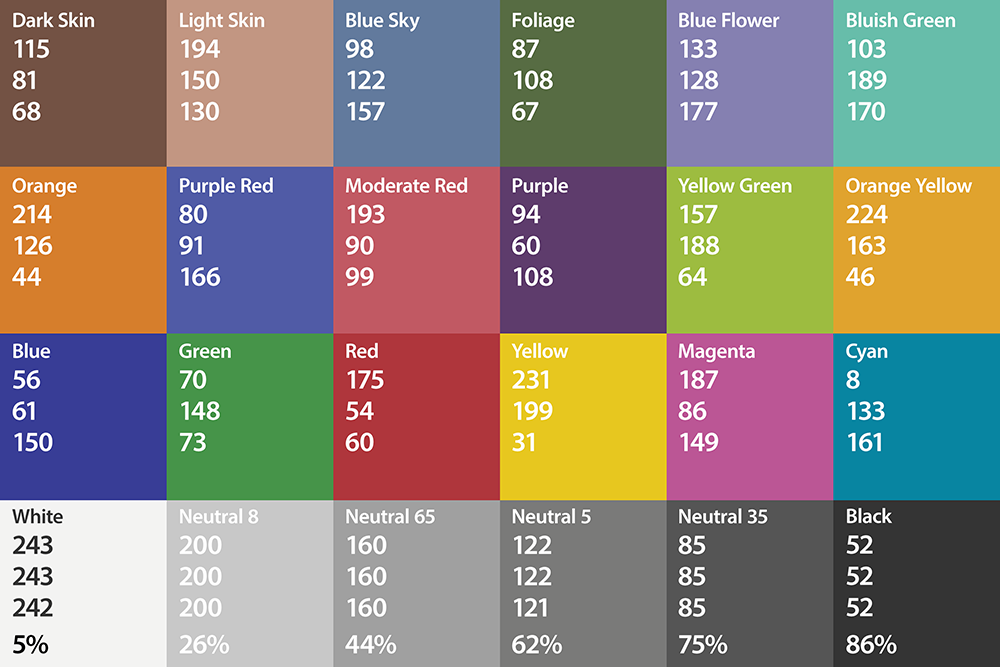
\includegraphics[width=7cm]{Figures/xritecolor chart RGB values.png}
%     \caption{Xrite color chart details for RGB values. The 75\% neutral gray has values of 0.33 (85/255) for Red Green Blue channels.}
%     \label{fig:xrite_description}
% \end{figure}

\begin{figure}[H]
    \centering
    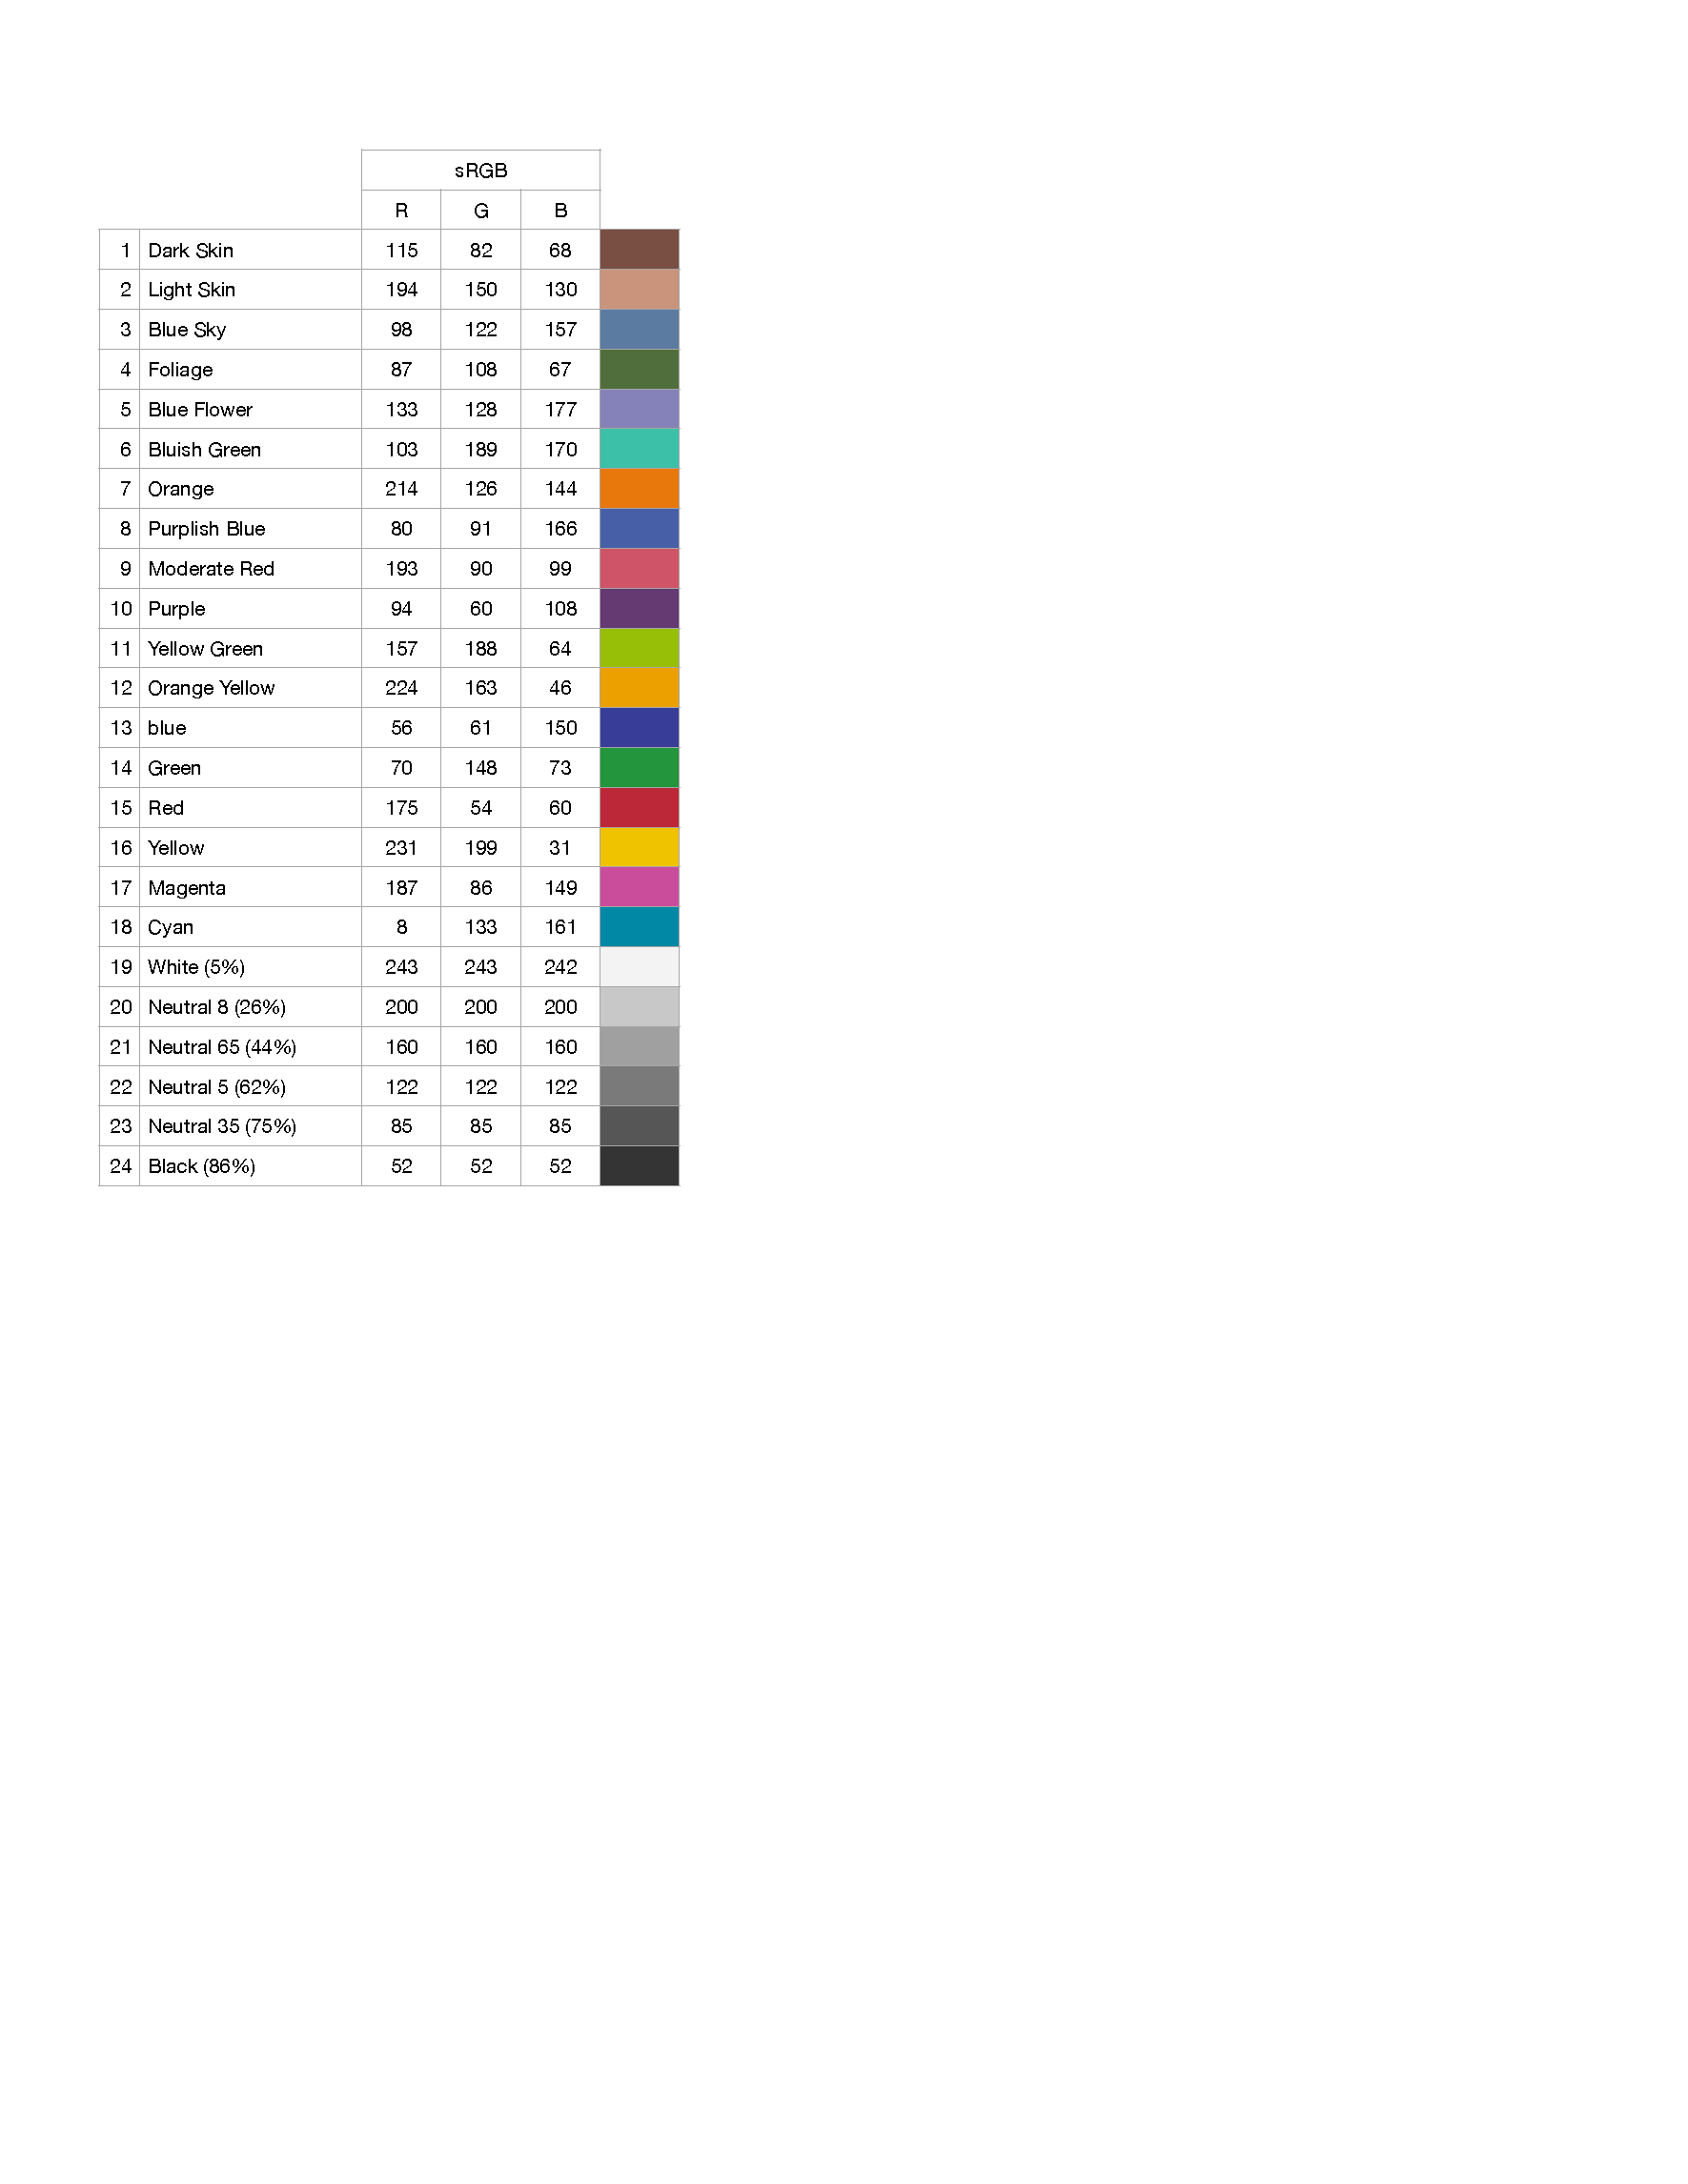
\includegraphics[width=7cm]{Figures/Color chart sRGB values.pdf}
    \caption{Xrite color chart details for standard Red Green and Blue (sRGB) values. The 75\% neutral gray has values of 0.33 (85/255) for Red Green Blue channels in the LightRoom software.}
    \label{fig:xrite_description}
\end{figure}



\subsection{Software}
To convert RAW photos (CR2 for Canon Raw Version 2 image files) to DNG files, we either use directly \href{https://www.adobe.com/ca_fr/products/photoshop-lightroom-classic.html}{Adobe Lightroom Classic} to export in DNG format the CR2 photos or \href{https://helpx.adobe.com/camera-raw/using/adobe-dng-converter.html}{Adobe DNG converter}. 
To calibrate the photos according to the color chart, we use the \href{https://xritephoto.com/ph_product_overview.aspx?ID=938&Action=Support&SoftwareID=2030}{Xrite Color Checker} software to create DCP camera profiles from DNG files, and Adobe Lightroom to use these profiles and apply them on an entire set of photos that need the same calibration.
To reconstruct the 3D models from photos, we use  \href{https://www.agisoft.com/downloads/installer/}{Agisoft Metashape}.


\begin{figure}[H]
\centering
\begin{subfigure}[t]{.33\textwidth}
  \centering
  
\includegraphics[width=0.4\textwidth]{Figures/logo Adobe DNG Converter.png}
  \caption{Adobe DNG Converter}
  \label{}
\end{subfigure}%
\begin{subfigure}[t]{.33\textwidth}
  \centering
  
\includegraphics[width=0.6\textwidth]{Figures/logo ColorChecker Camera Calibration.png}
  \caption{ColorChecker Camera Calibration}
  \label{}
\end{subfigure}
\begin{subfigure}[t]{.33\textwidth}
  \centering
  
\includegraphics[width=0.3\textwidth]{Figures/logo Lrc.png}
  \caption{Adobe Lightroom Classic}
  \label{}
\end{subfigure}
\caption{Software for color calibration}
\label{}
\end{figure}



\subsection{Flowers}

Collect fresh flowers from the plant, label them and store them in a cool place or with the tip of the peduncle in some water to prevent accelerated wilting. Different flowers will wilt at different paces.
Flowers are pinned through the floral receptacle or peduncle using entomological pins in dense foam at the center of the turntable. Alternatively, flowers can be secured in a truncated pipette tip, itself fixed on the turntable, or with alligator clips to rapidly fix the flowers.

\begin{tcolorbox}[width=\linewidth, colback=mygray,title=Suggestion for the Joly Lab,colframe=lightgray] %sharp corners=uphill pour avoir juste un coin sur deux de sharp
Store flowers in 50mL Eppendorf tubes or in foam box no more than an hour before taking photos of them.\\
\\
In some cases, it is necessary to remove sepals from the flower before building the model to accurately study the corolla shape. To do this, use a razor blade and mark the sepal intersections with a waterproof pen. The marks will help for the model construction and more importantly landmarks positioning.
\end{tcolorbox}



\subsection{Summary of materials and software}
%prices : vary according to websites, and time..
%some are depending on the flowers and materials needed to have it fixed on the table.. pinces/mousse/aiguille/...
\begin{table}[H]
\begin{tabular}{L{5cm}|L{9cm}|C{1.7cm}}
\textbf{Material} & \textbf{Description} & \textbf{Price (USD)} \\\hlinewd{1pt}

\multicolumn{1}{l}{\textbf{Photography}}\\\hlinewd{1pt}
Camera & Digital Single-Lens Reflex (DSLR), e.g. Canon t2i & e.g. \$500 \\\hlinewd{0.1pt}
Macro lens & A preferably fixed lens, e.g. Canon 60mm f/2.8 Macro lens & e.g. \$400 \\\hlinewd{0.1pt}
Tripod & Preferably flexible, such as a gorillapod & e.g. \$80 \\\hlinewd{0.1pt}
Stepping motor and turntable kit & \href{https://www.bhphotovideo.com/c/product/1486043-REG/syrp_sykit_0043_genie_mini_ii_turntable.html/quick-compare}{Genie mini II}, Shoot smooth rotating video and interactive 360\degree\hspace{0.01cm} images of objects. Full iOS and Android App control via Bluetooth. Battery life: 6hrs video and 15hrs time-lapse. Panning payload 8.8lbs/4kgs & \$328.00 \\\hlinewd{1pt}
Lightbox & A portable photo studio, e.g. \href{https://neewer.com/products/lighting-studio-10094456?_pos=2&_sid=bde9f6ddb&_ss=r}{Neewer} 20"/50cm foldable portable photography lighting kit (Neewer Technology Co. LTD, Shenzhen,  China), adjustable brightness with 120 LED lights, CRI (colour Rendering Index) of 85+, 6000-6500K colour temperature, needs to be powered by a portable battery in the field, white and grey backdrops & \$79.99 \\\hlinewd{0.1pt}
External battery & Powering source for in-field photo capture, essentially for the lightbox or to recharge batteries & optional \\\hlinewd{1pt}

\multicolumn{1}{l}{\textbf{Flower mounting and identification}}\\ \ChangeRT{1pt}
Flower & Freshly cut flower with peduncle and floral receptacle & / \\\ChangeRT{0.1pt}
Labels and container & Identification and storage of fresh flowers to avoid damage and avoid wilting & / \\\ChangeRT{0.1pt}
Turntable labels & Identification to species, collector, collection number, date, locality, and coordinates, and the chunk number. To use as a separate photo before each run of photos. & / \\\ChangeRT{0.1pt}
Razor blade & To remove sepals & / \\\ChangeRT{0.1pt}
Small block of dense foam & To fix flowers in place with a pin at the center of the turntable.  & / \\\ChangeRT{0.1pt}
Entomological pins & To pin through the peduncle or floral receptacle and fix the flower on the turntable. & / \\\hlinewd{0.1pt}
Scale & A 1 cm scale as reference & / \\\hlinewd{1pt}

\multicolumn{1}{l}{\textbf{Color calibration}}\\\hlinewd{1pt}
Color chart & A color reference to calibrate RAW photos (e.g. \href{https://www.xrite.com/categories/calibration-profiling/colorchecker-targets/colorchecker-passport-photo-2}{X-rite ColorChecker Passport}) & e.g. \$99.00 %verify price 90$
\\\hlinewd{0.1pt}
Color calibration software & ColorChecker Camera Calibration, Xrite software for automatic color profile creation & Free \\\hlinewd{0.1pt}
Photo editing software & Adobe Photoshop Lightroom, editing software for image color calibration in batch & Payment plans vary  \\\hlinewd{1pt}
DNG conversion software & Adobe DNG converter, to convert Camera Raw files from supported cameras to the more widely used DNG raw files & Free \\\hlinewd{1pt}

\multicolumn{1}{l}{\textbf{Model reconstruction}}\\ \ChangeRT{1pt}
3D reconstruction from photogrammetry software & Agisoft Metashape Pro Software & \$549 Academic price \\\hlinewd{0.1pt}
\end{tabular}
\caption{\label{table:listOfMaterials} Summary of the materials used to scan and reconstruct flower three-dimensional models and their price. Alternative materials can be considered, and we give as an example the specific materials that we used when relevant.}
\end{table}




\newpage
\section{Settings and preparation}

\subsection{Camera and tripod settings and preparation}
%what you need
To obtain the best picture quality for model reconstruction, we need an optimal combination of the light sensibility of the sensor (ISO), the duration of exposure and the focal of the objective (F). As mentioned, it is preferable to use a fixed lens (one that doesn't allow zooming) to facilitate the model reconstruction in the processing step because the software can't take zooming into account in the reconstruction process.
Maximizing the light source allows us to use the lowest ISO to get crisper images. Adapted time exposure to allow the right amount of light to go to the sensor, avoids low key nor high key photo (under/over exposed photo). This may be adapted according to the subject (light or dark colored subject or background) or if different lighting conditions are used.

To maximize the depth of field without lowering the image quality, using the manual option on the camera dial, the focal F should be set to F16. Use the manual focus setting on the side of the lens (Figure \ref{camera_arrows}) to avoid camera trigger malfunction when the flowers doesn't land on the detector. If the flower is off centered during rotation, and the automatic focus can't focus (on the background) the camera trigger is prevented with the automatic focus. On manual, the camera will always be triggered by the turn table, even if the focus isn't optimal. Because the subject is moving and may be off centered on the turntable, the focus may need to be adapted while the turn table runs. For this you can pause the turntable, manually adjust the focus, and resume the spin.
%Using white balance target in the color chart, you can set a personalized white balance for your camera.


A flexible tripod (Figure \ref{tripod}) is used to adjust several camera heights, high, middle, and low, close to the subject.

\begin{figure}[H]
\centering
\begin{subfigure}[t]{.5\textwidth}
  \centering
  \includegraphics[width=6cm]{Figures/camera_arrows.png}
  \caption{Camera and lens used to take RAW photos. The red arrows (from top to bottom) depict the button to get manual focus, the ISO button and the manual parameter on the camera dial.}
  \label{camera_arrows}
\end{subfigure}%
\begin{subfigure}[t]{.5\textwidth}
  \centering
  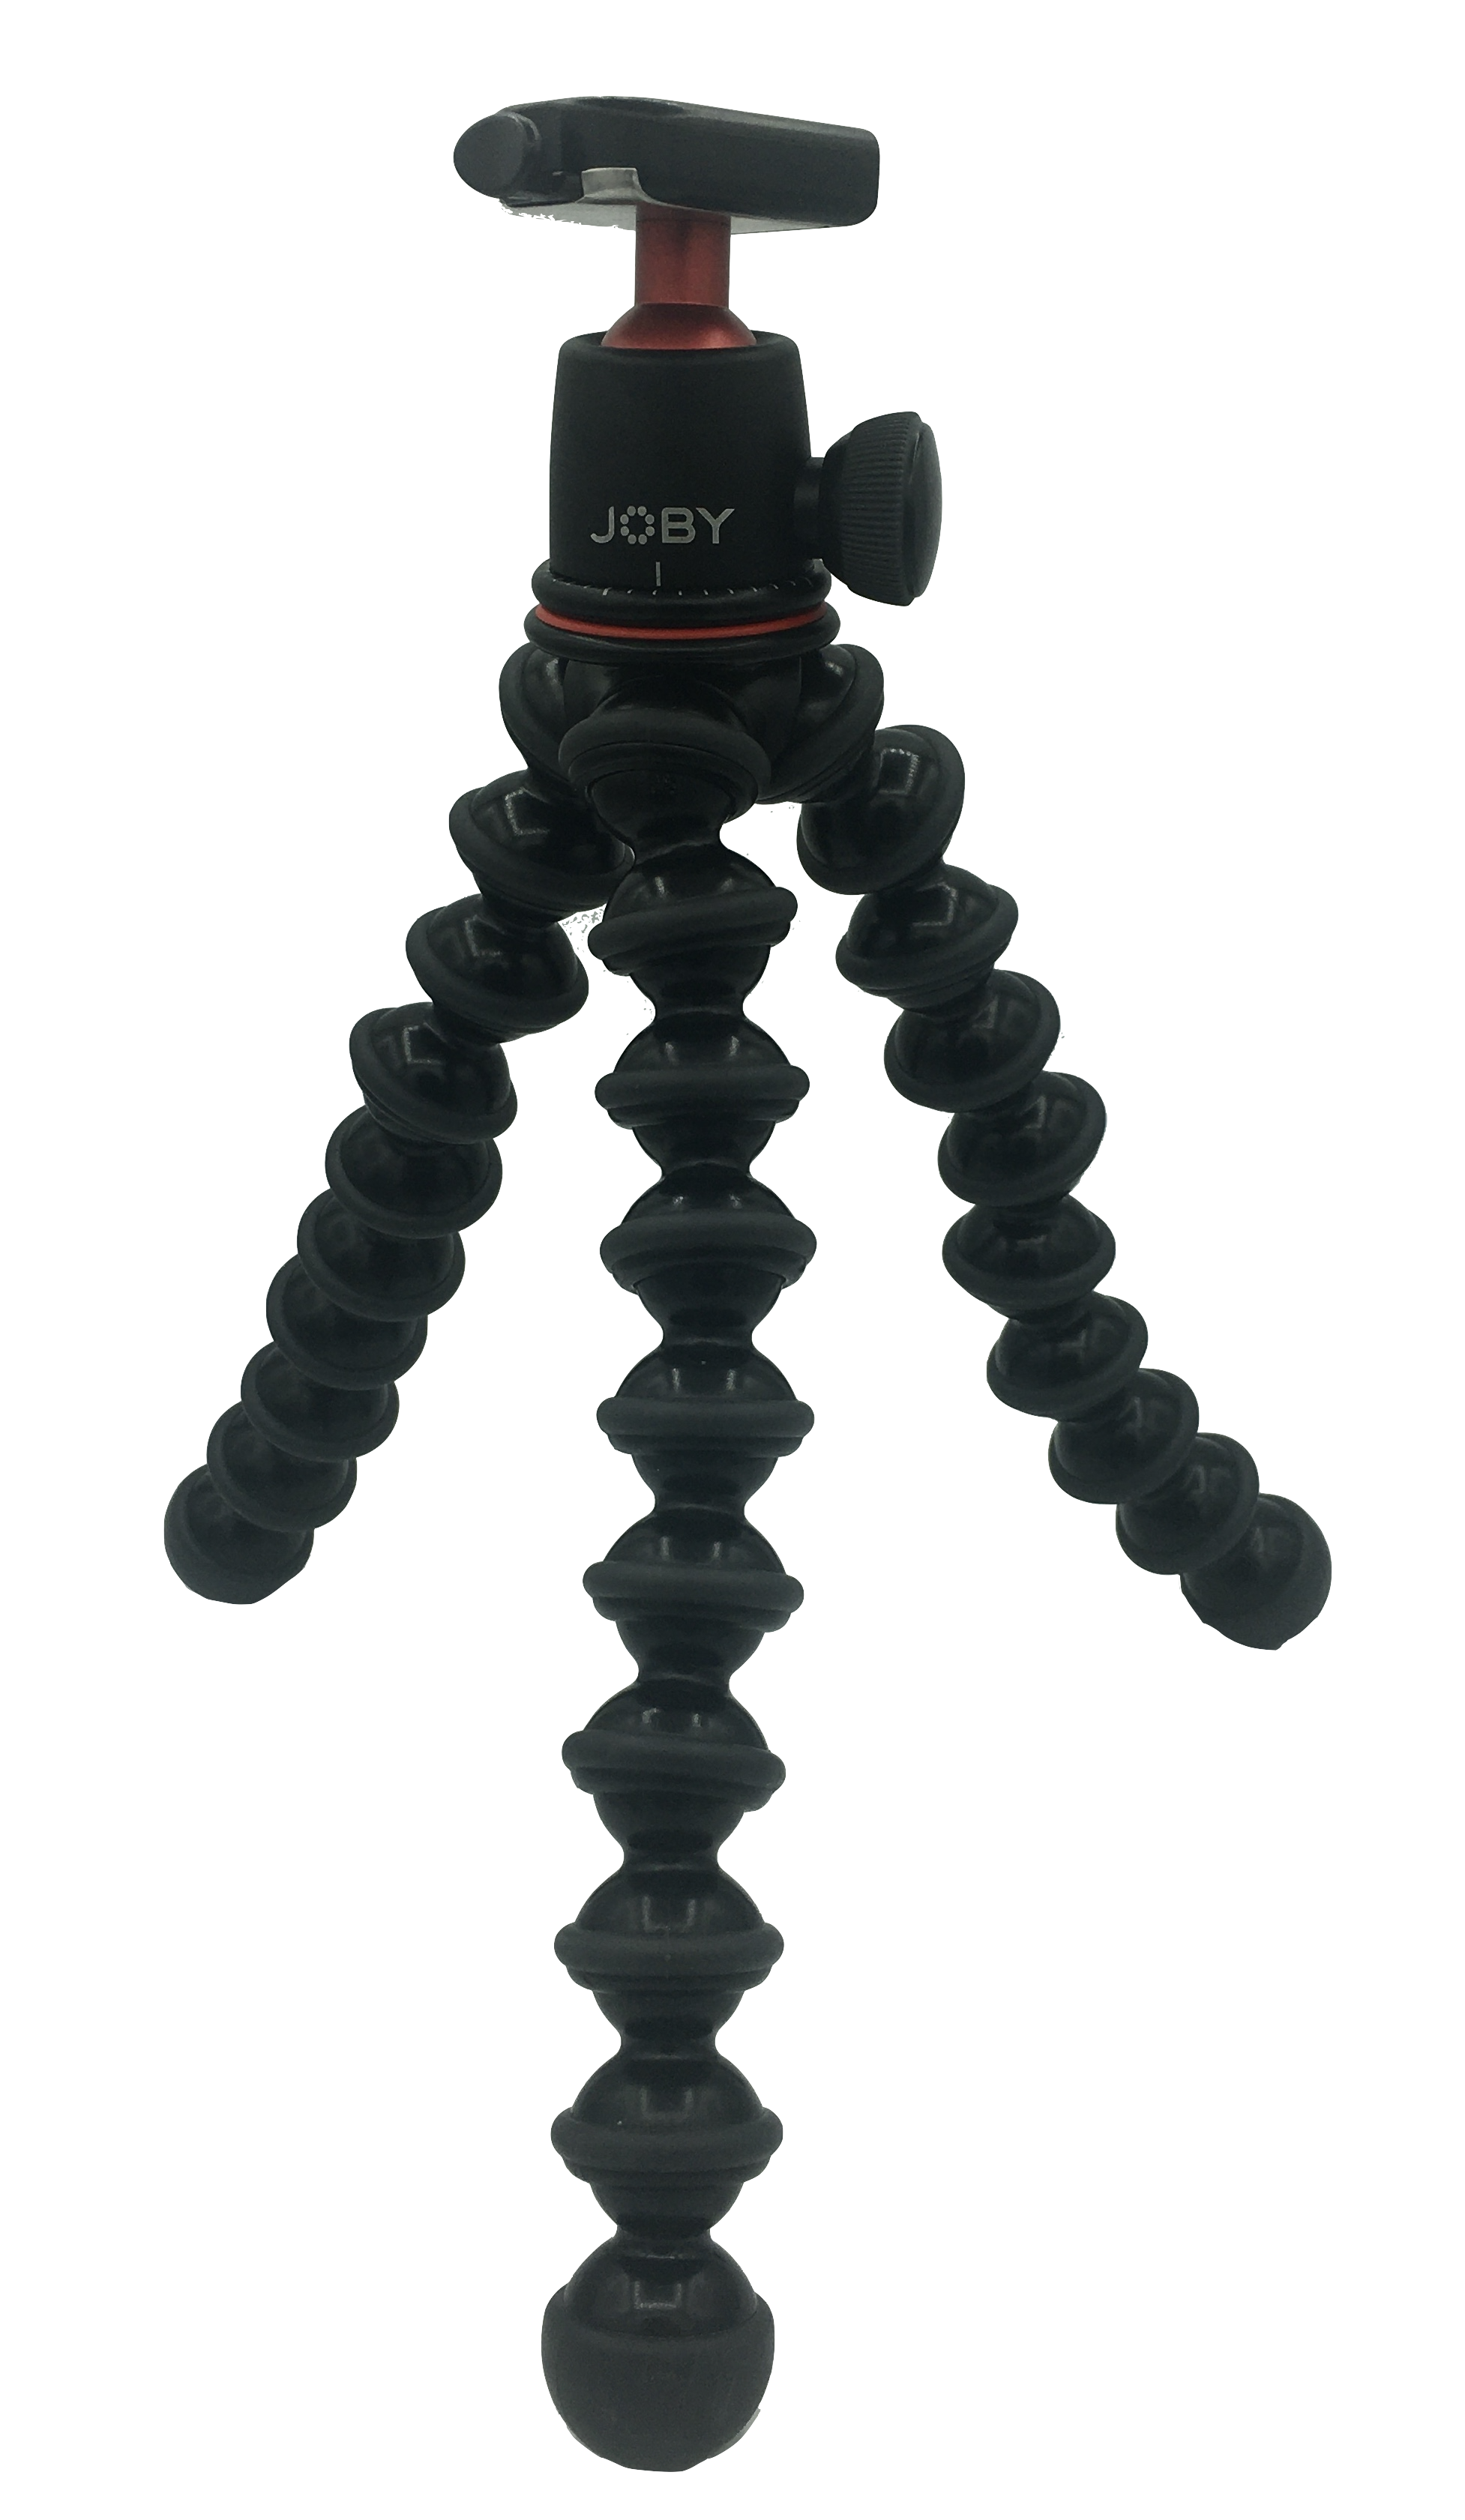
\includegraphics[width=4cm]{Figures/tripod.png}
  \caption{Flexible tripod used to adjust camera positions.}
  \label{tripod}
\end{subfigure}
\caption{Photo capture materials : camera, lens, and tripod}
\label{}
\end{figure}




\subsubsection{Camera settings}
The standard settings have to be adjusted depending on the flower (colour mostly and conditions). We often use the following settings : exposure time (shutter speed) 1/20s, F/16 focal, ISO 100, standard exposition on the light meter, and we save pictures as RAW files (ML setting on the camera display) format to be able to post-process them for color calibration (Figure \ref{fig:my_label}). A RAW photo of the color chart with an identical set of lighting conditions and camera settings as the flower to be photographed is needed for each flower photos series. If several flowers are processed one after the other without variation of light conditions, only one chart photo is needed.


\begin{tcolorbox}[width=\linewidth, colback=mygray,title=Tip,colframe=lightgray] %sharp corners=uphill pour avoir juste un coin sur deux de sharp
The nicer and the sharper the photographs, the easier it will be to build the models. So make sure that the flower is always in focus. Shade or high light reflectance can also impair model reconstruction, so pay attention to these while taking the pictures.
\end{tcolorbox}

\begin{figure}[H]
    \centering
    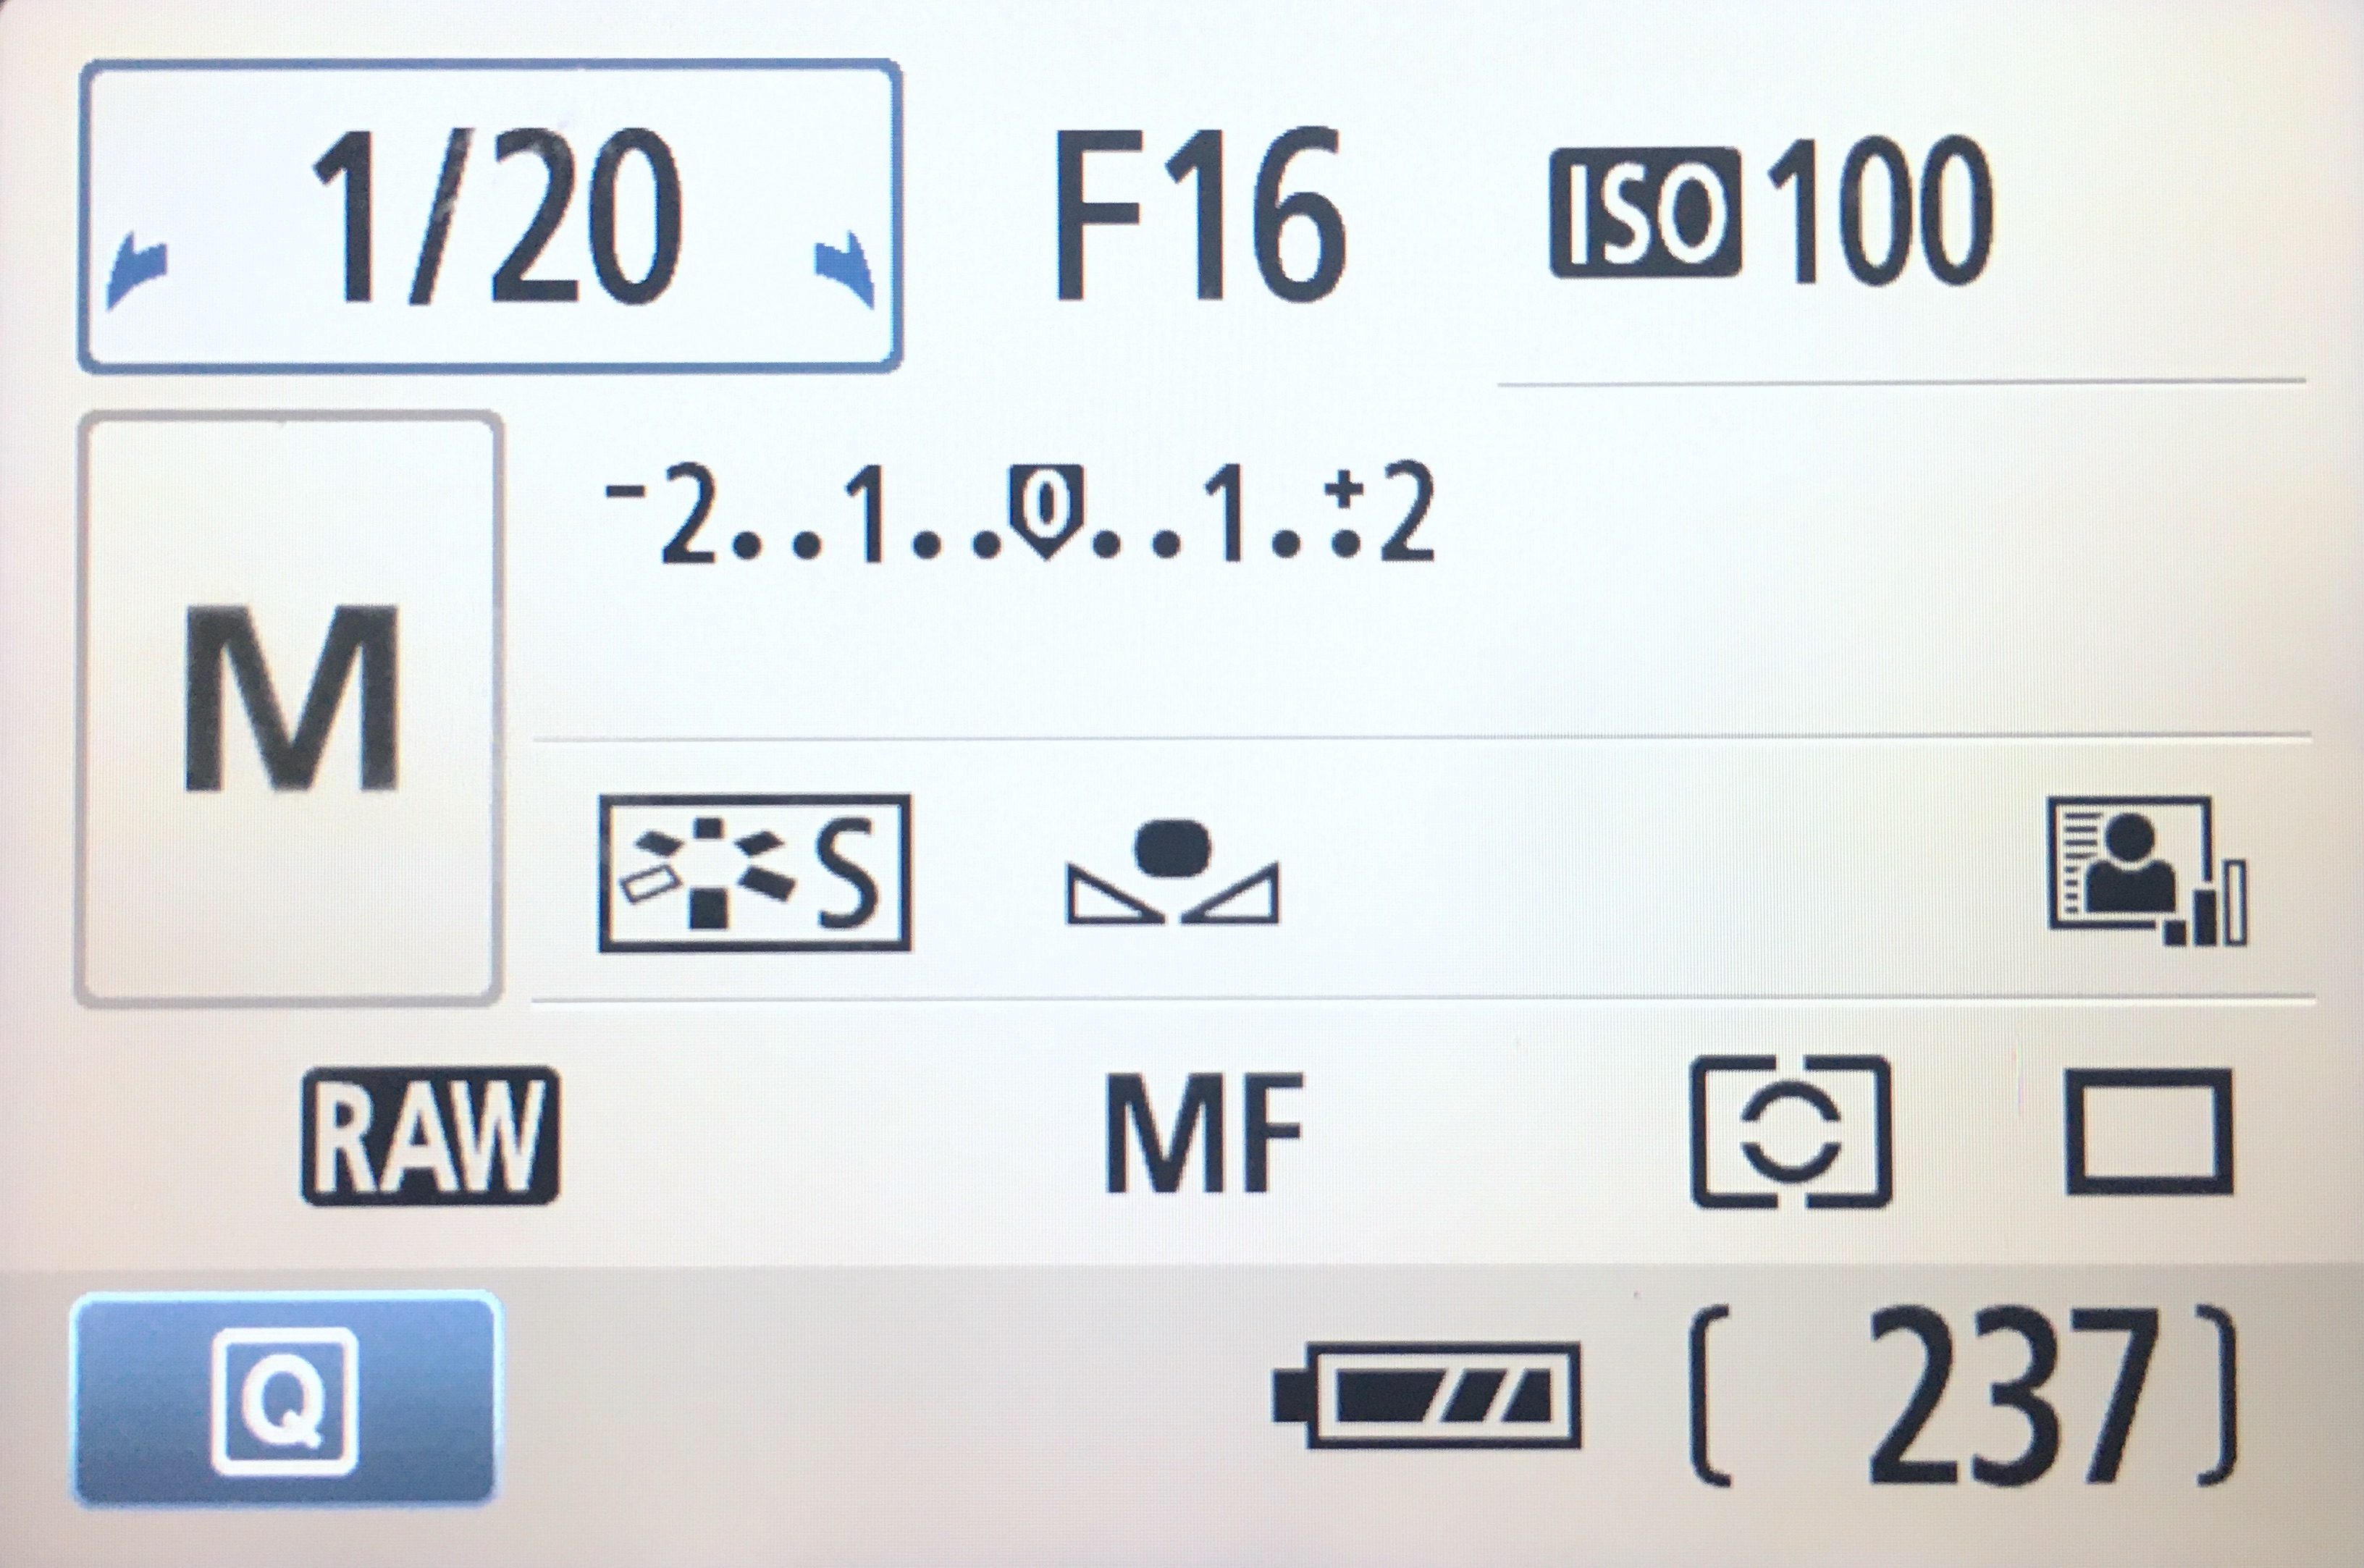
\includegraphics[width=0.5\linewidth]{Figures/camera_settings.JPG}
    \caption{Camera settings interface of the Canon t2i/550D}
    \label{fig:my_label}
\end{figure}




\subsubsection{Optional : custom camera white balance}
Optionally, you can begin by setting a personalized white balance in your camera with the light gray scale on the chart :
\begin{enumerate}
    \item For a Canon camera, take a picture of the gray scale
    \item Choose \textit{Custom WB} in your camera settings (Figure \ref{WB_sub1})
    \item Select \textit{Custom} and use the picture of the grey scale to define your custome white balance (Figure \ref{WB_sub2}).  Be careful, you will still require to linearize and calibrate each photo afterwards.
\end{enumerate}

However, the color chart will always be the reference for post-processing the color calibration of each photo. This optional section only helps to have a better preview of the photos.

\begin{figure}[H]
\centering
\begin{subfigure}[t]{.5\textwidth}
  \centering
  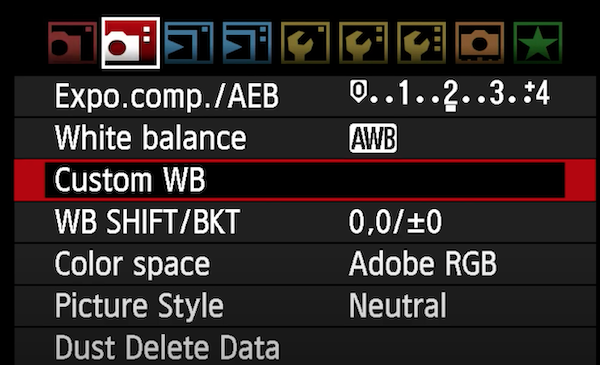
\includegraphics[width=7cm,height=4.5cm]{Figures/Custom WB setting.png}
  \caption{Custom WB parameter}
  \label{WB_sub1}
\end{subfigure}% -> this % allows the graphs to be side by side as opposed to one on top of the other
\begin{subfigure}[t]{.5\textwidth}
  \centering
  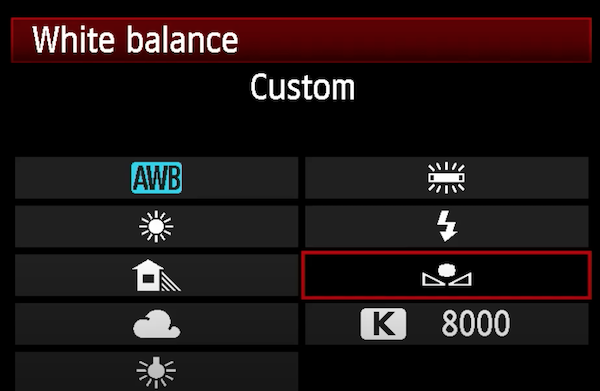
\includegraphics[width=7cm,height=4.5cm]{Figures/Custom WB selection.png}
  \caption{Select your custom WB}
  \label{WB_sub2}
\end{subfigure}
\caption{White balance customization on a Canon t2i camera interface}
\label{WB}
\end{figure}



\subsection{Turn table settings and preparation}

For each run (one 360\degree\hspace{0.01cm} spin of the turn table), we use a wait time of 2s to allow the camera time to save the images on the SD card after it is triggered, and the flower to stabilize after each rotation.

\begin{enumerate}
    \item Connect the shutter release to your camera and the turntable Syrp Genie II (Figure \ref{fig:shutter}).
    \item Turn the turntable on (to turn it off, hold the \textit{on} button for 3 seconds).
    \item Connect the Syrp Genie II to your device, and do the updates if required (needs an internet connection).
    \item Click on \textit{create content} > \textit{turntable} (Figure \ref{genie_root}, \ref{genie_content}).
    \item In parameters (Figure \ref{record}), select 20 photos for each run, and 2s of waiting (move-wait-shoot-wait-move). If it is too quick, some pictures won't be able to be saved as the camera needs a delay to save them on the memory card. The spinning device will take the first picture then proceed to a move-shoot-move run until the last photo.%add details here
    %According to the exposure time, the duration of the pause between each move has to allow enough time for the camera to take the picture.
    \item Place the white background circle on the turntable to contrast with the flower. If your flower is pale, then use a different background (colored or darker). Ideally, the color of the circle should be the exact same color of the background of the lightbox as this will help when applying masks later.
\end{enumerate}


\begin{figure}[H]
    \centering
    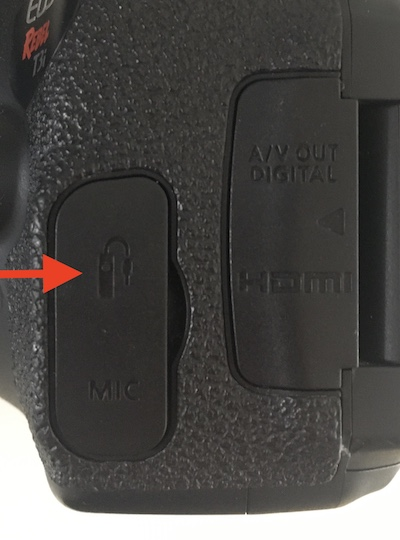
\includegraphics[width=0.3\textwidth]{Figures/shutter.jpg}
    \caption{Camera shutter release port}
    \label{fig:shutter}
\end{figure}

\begin{figure}[H]
     \centering
     \begin{subfigure}[b]{0.48\textwidth}
         \centering
         
\includegraphics[width=\textwidth]{Figures/genie_root.PNG}
         \caption{Genie app interface root}
         \label{genie_root}
     \end{subfigure}%
\hfill
     \begin{subfigure}[b]{0.48\textwidth}
         \centering
         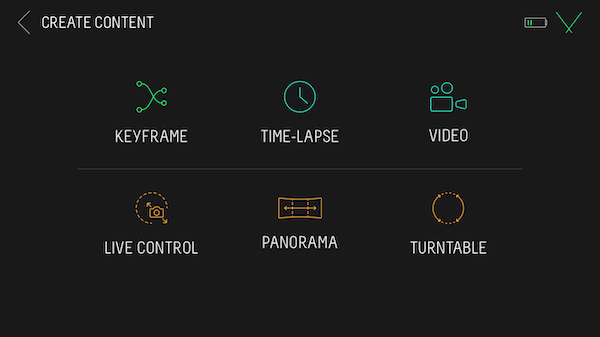
\includegraphics[width=\textwidth]{Figures/genie_create.PNG}
         \caption{Create turntable content}
         \label{genie_content}
     \end{subfigure}
\\
    \begin{subfigure}[b]{0.48\textwidth}
         \centering
         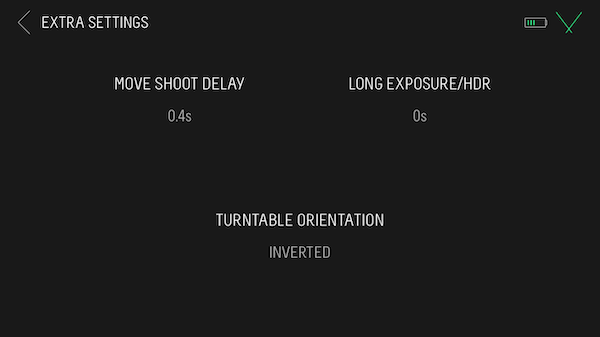
\includegraphics[width=\textwidth]{Figures/genie_settings.PNG}
         \caption{Genie detailed settings}
         \label{fig:genie_settings}
    \end{subfigure}%
\hfill
    \begin{subfigure}[b]{0.48\textwidth}
         \centering
         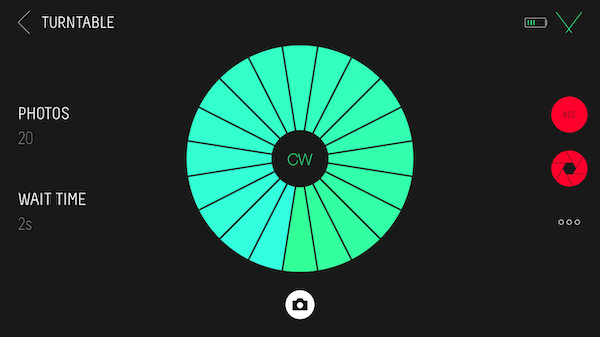
\includegraphics[width=\textwidth]{Figures/genie_turntable_20_1.PNG}
         \caption{Start recording with the turntable}
         \label{record}
     \end{subfigure}
        \caption{Turntable setup and settings via the Syrp smartphone application}
        \label{turntable}
\end{figure}




\subsection{Summary of settings}

\begin{table}[H]
\begin{tabular}{L{4cm}|L{12cm}}
\textbf{Parameter} & \textbf{Description} \\ \hlinewd{1pt}
\multicolumn{1}{l}{\textbf{Camera settings}} \\ \ChangeRT{1pt}
Aperture & F/16 \\\hlinewd{0.1pt}
Sensibility & ISO 100 (lowest)\\\hlinewd{0.1pt}
Exposure time & 1/20s - Can be adapted according to the flower. \textbf{Reminder} : a photo of the color chart in the exact same light conditions and camera parameters as the flower needs to be taken. \\\ChangeRT{1pt}
\multicolumn{1}{l}{\textbf{Turn table settings}} \\ \ChangeRT{1pt}
Number of photos & 20 per 360\degree \hspace{0.01cm} for one camera position and one flower position. May be adjusted according to each flower.\\\hlinewd{0.1pt}
Wait time & 2s\\\hlinewd{0.1pt}
\end{tabular}
\caption{\label{table:cameraSettings} Summary of the camera and turn table settings.}
\end{table}






\section{Image capture step-by-step}

\subsection{Take a picture of the color chart}
\begin{enumerate}
    \item Set the camera settings to F/16, ISO 100, 1/20s, and RAW format.
    \item Verify that you have enough space on your SD card for RAW photos (a minimum of 163 photos, accounting for photos of labels and chart).
    \item Verify that the placement of your turntable inside the lightbox will allow to capture correctly the flower you are about to photograph (distance from opening of the lightbox) and that the 1/20s shutter speed captures enough light from your flower by taking an initial photo of your flower.
    \item If satisfactory go to next step. The goal here is to have a definite set of settings that will match both your flower photos and a color chart to subsequently calibrate all your photos that have the same light conditions and camera settings.
   \item Place the color chart where the flower will be placed, without shadows, and exposed under the same light as the flower will be (angled towards the LED source light in the lightbox). The camera settings and lighting cannot be changed after this. If the lighting or the camera settings are modified, the color chart needs to be taken again to correct the corresponding photos.
   \item Place the camera so that the entire chart is visible.
   \item Take a picture of the color chart (RAW). Make sure to Incorporate each color squares, and the corners of the chart as follows (Figure \ref{colorchart}).
   \end{enumerate}


\begin{figure}[H]
\centering
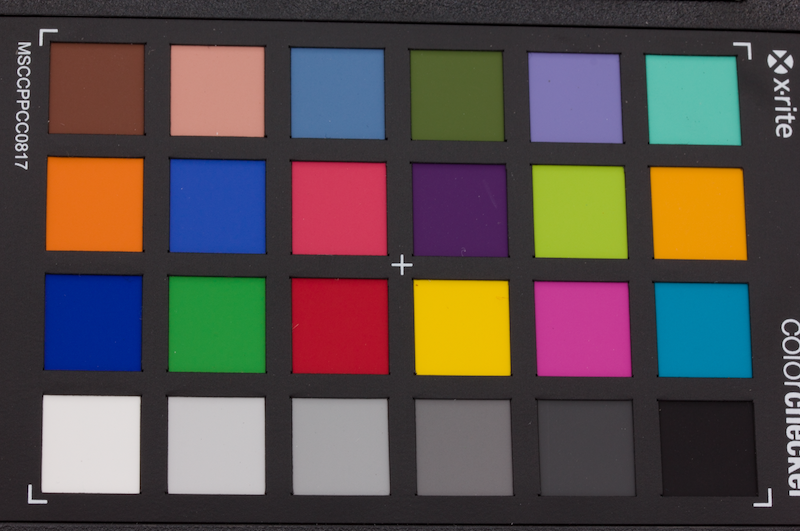
\includegraphics[width=0.3\textwidth]{Figures/chart_example.png}
\caption{Colour chart photo taken at the beginning of the process to calibrate the photos in post process.}
\label{colorchart}
\end{figure}







\subsection{Flower placement \& Image capture}
  
To reconstruct an accurate 3D model, it is very important to have pictures of all the parts and details of the flowers and from several angles. Also, the photographs need to overlap with each other for proper alignment in the first steps of the reconstruction. For this reason, several pictures will be taken of each flower: from different orientation and all around the flower.
We suggest that flowers should be photographed from at least two positions. Note that it is better to take more photos than less because if we can drop some pictures during the model reconstruction, it is impossible to come back and take more pictures if we realize that we should have taken more.


\begin{tcolorbox}[width=\linewidth, colback=mygray,title=Suggestion for the Joly Lab,colframe=lightgray]
For Gesneriaceae, we first suggest a standard orientation and an upside-down position of the flower as this generally gives satisfactory results (Figure \ref{flowerplacement_2}). For more complex flowers, three positions may be required: horizontal, vertical, and upside down (Figure \ref{flowerplacement_3}).
\end{tcolorbox}


\begin{enumerate}
    \item Clip the camera on the flexible tripod (gorillapod) and place the camera at one of the three position required per flower position : high mid, and low position (see Figure \ref{flowerplacement_2}). Make sure to not use different camera orientations (landscape vs. portrait).
    %FIGURE OF POSITIONS.
    \item If sepals need to be removed, use a razor blade to cut them at the base and mark the sepal intersections with a waterproof pen to keep track of the morphological structures.
    \item Pin the flower through the peduncle or the floral receptacle and through a block of dense foam or malleable gum. You can use several pins to avoid any sliding of the flower during the image capture process.
    \item Make sure to place the flower so that the whole flower will be encompassed in the camera frame as much as possible. It is best to have the subject to take the most place as possible in the camera frame to capture every details overall than having it entirely in the camera frame but with poor detail quality. What counts the most is to get several overlapping photos for each features. Make sure that the flower is not in contact with anything as this would deform the flower and create problems during the model reconstruction.
    \item For flowers with very uniform color or with radial symmetry, it may be important to place dots with a waterproof pen on the corolla to facilitate manual marker positioning and/or automated pixel position detection in the reconstruction step.
    \item Place a scale (e.g., 1 cm) directly below the flower.
    \item Take a picture of the flower with the label for each new positioning of the flower. This will help to identify each group of images in the following model construction.
    \item Press the \textit{rec} button on your smartphone using the turntable interface to start the spin of the turntable and automated image capture.
    \item Verify occasionally the focus on the flower while the flower rotates by pressing the square button (stop) and manually adjust the focus if needed, then press rec to resume your spin.
\end{enumerate}


%FIGURE of the 3 positions of the camera

\begin{figure}[H]
\centering
\begin{subfigure}[t]{.33\textwidth}
  \centering
  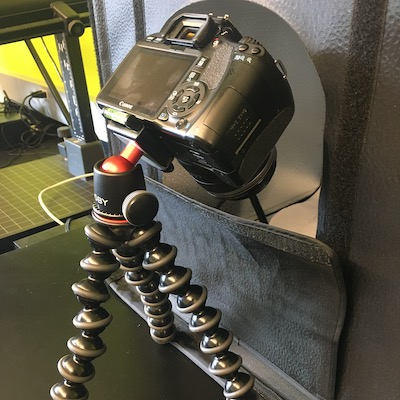
\includegraphics[width=0.9\textwidth]{Figures/camera_position_1.JPG}
  \caption{}
  \label{}
\end{subfigure}% -> this % allows the graphs to be side by side as opposed to one on top of the other
\begin{subfigure}[t]{.33\textwidth}
  \centering
  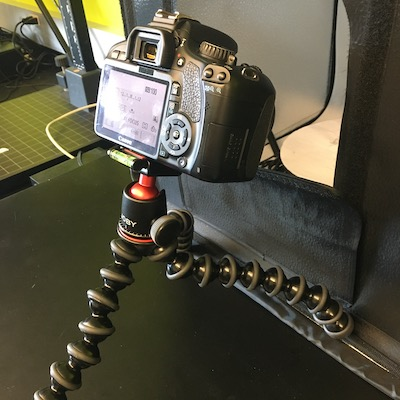
\includegraphics[width=0.9\textwidth]{Figures/camera_position_2.JPG}
  \caption{}
  \label{}
\end{subfigure}%
\begin{subfigure}[t]{.33\textwidth}
  \centering
  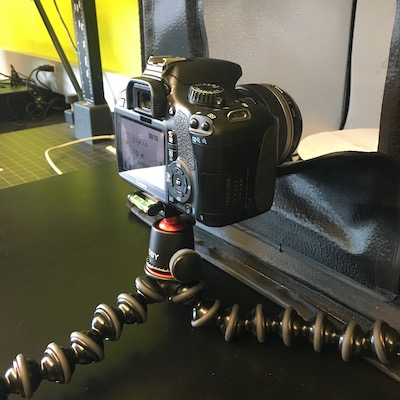
\includegraphics[width=0.9\textwidth]{Figures/camera_position_3.JPG}
  \caption{}
  \label{}
\end{subfigure}
\caption{Camera positions}
\label{flowerplacement_2}
\end{figure}



%FIGURE of dorsal + ventral view
\begin{figure}[H]
\centering
\begin{subfigure}[t]{.5\textwidth}
  \centering
  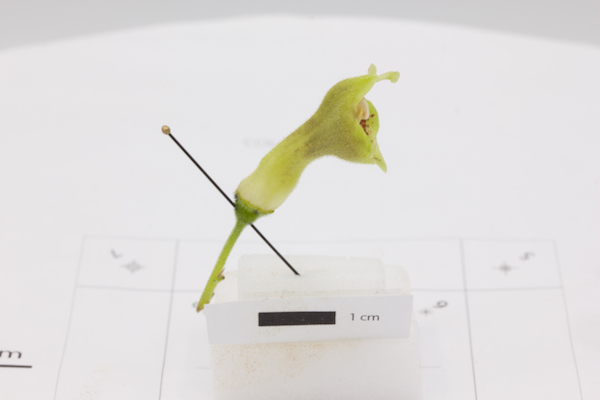
\includegraphics[width=0.9\textwidth]{Figures/position_2.jpg}
  \caption{}
  \label{}
\end{subfigure}%    -> this % allows the graphs to be side by side as opposed to one on top of the other
\begin{subfigure}[t]{.5\textwidth}
  \centering
  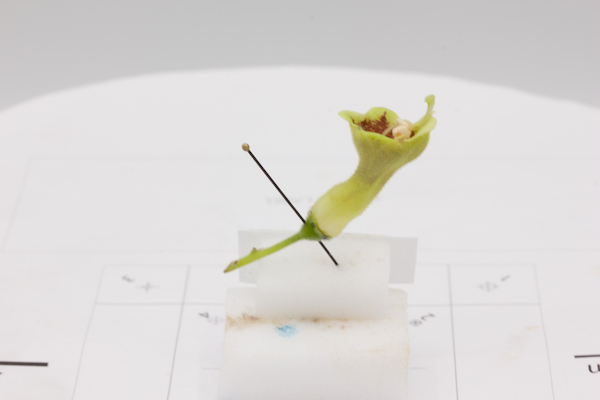
\includegraphics[width=0.9\textwidth]{Figures/position_5.jpg}
  \caption{}
  \label{}
\end{subfigure}
\caption{Usual flower positions on ventral and dorsal view, for two distinct chunks of photos, but with 3 different camera positions each.}
\label{flowerplacement_3}
\end{figure}



%FIGURE of dorsal view + vertical + ventral view (exception).
\begin{figure}[H]
\centering
\begin{subfigure}[t]{.33\textwidth}
  \centering
  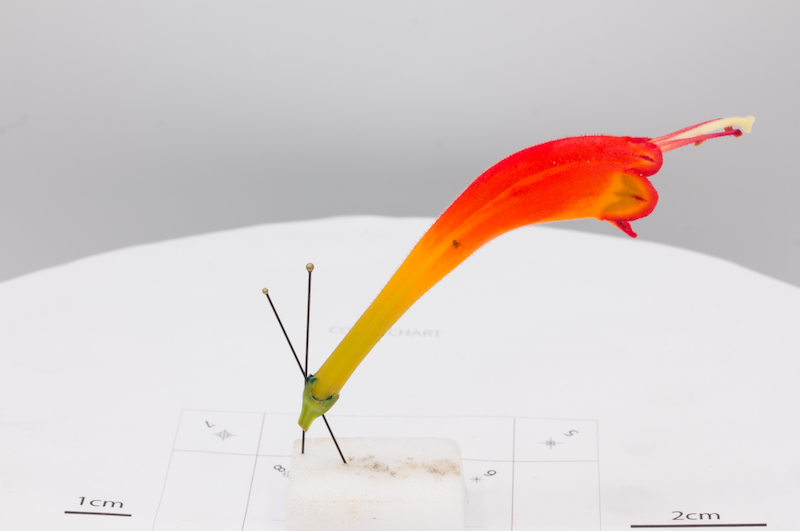
\includegraphics[width=0.9\textwidth]{Figures/flowerplacement_1.png}
  \caption{}
  \label{}
\end{subfigure}% -> this % allows the graphs to be side by side as opposed to one on top of the other
\begin{subfigure}[t]{.33\textwidth}
  \centering
  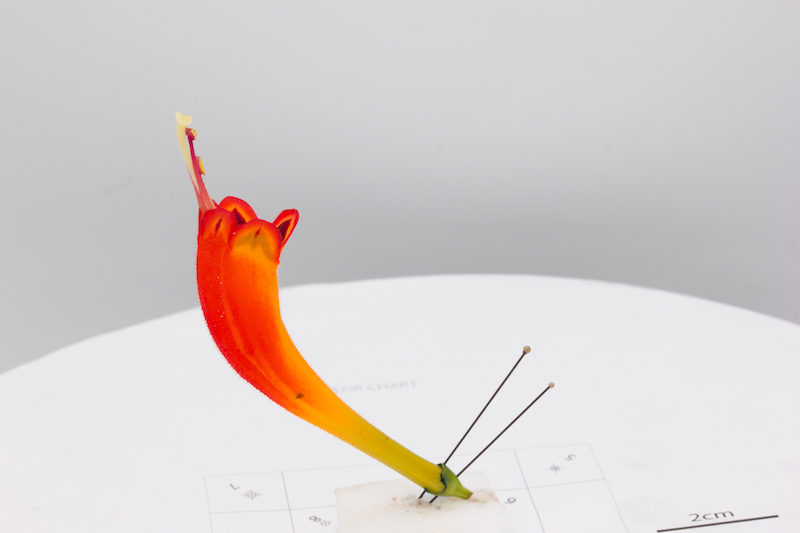
\includegraphics[width=0.9\textwidth]{Figures/flowerplacement_2.jpg}
  \caption{}
  \label{}
\end{subfigure}
\begin{subfigure}[t]{.33\textwidth}
  \centering
  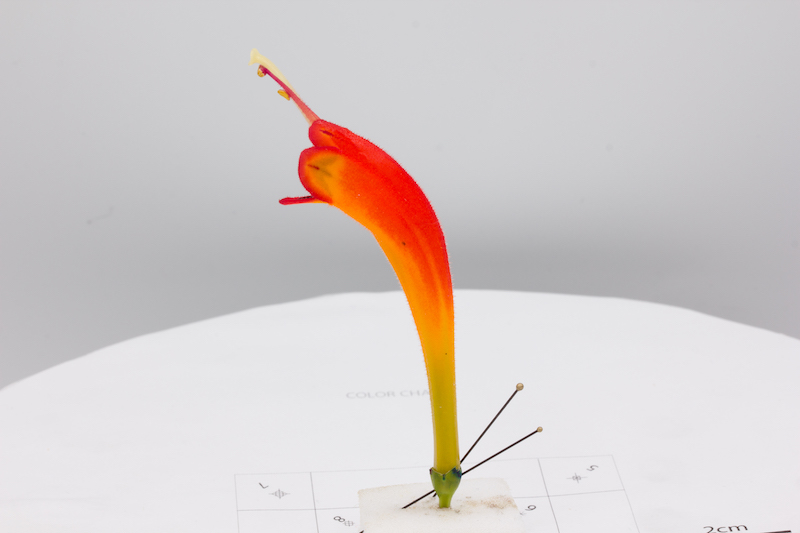
\includegraphics[width=0.9\textwidth]{Figures/flowerplacement_3.jpg}
  \caption{}
  \label{3placement}
\end{subfigure}
\caption{Flower placement for three distinct chunks of photos for flowers that are difficult to place on ventral and dorsal view only.}
\label{flowerplacement}
\end{figure}



\begin{tcolorbox}[width=\linewidth, colback=mygray,title=Suggestion for the Joly Lab,colframe=lightgray] %sharp corners=uphill pour avoir juste un coin sur deux de sharp
Adjust the number of flower positions and number of photos according to each flower. For intricate flowers, or flowers that can't be captured entirely with only two positions (ventral and dorsal), you can place the flower on an another position (Figure \ref{3placement}). On the contrary, if the flower can't be placed on several positions, you may need to increase the number of photos per camera height in order to have sufficient information for the software to reconstruct accurate 3D models.
\end{tcolorbox}






\section{Image post processing}
\subsection{File names and storage}

%%%%%ADD DETAILS 

We found that it is critical to have a very organized structure for saving files, especially when several persons are working on the same project. We propose here what has been working so far for us.

In a species folder named with the name of the species (\textit{Genus\_species}), there should be a distinct folder for each individual photographed, usually with a different collection number. If the same individual has been photographed several times, the date of photos acquisition should be appended to the folder name to discriminate them. We also indicate with the folder name if the individual has been photographed with or without sepals.

For each flower, we have one folder for uncalibrated photos, one for calibrated photos, and one for the model. The picture of the color chart should be placed in the uncalibrated photos.

To distinguish which photo goes in which chunk, a photo of the label is taken at the beginning of each chunk (each set of photo per side of flower). We suggest to place the photos from different chunks in different folders, once the photos are calibrated. The date of when the photos are taken is important because it helps matching the calibration to the right DNG file. If more than one set of photos with different lighting or camera settings are taken, make sure to distinguish the color charts that correspond to each set of photos.

\begin{tcolorbox}[width=\linewidth, colback=mygray,title=Suggestion for the Joly lab: example of file organization,colframe=lightgray]
Genus\_species\\
\hspace*{1cm} GEN\_species\_CollectionNumber\\
  \hspace*{2cm} sepal\_DD.MM.YYYY or no\_sepals\_DD.MM.YYYY\\
    \hspace*{3cm} Model\\
        \hspace*{4cm} \textit{MetashapeProject}\\
        \hspace*{4cm} \textit{MetashapeProjectFolder.files}\\
        \hspace*{4cm} \textit{model.obj}\\
        \hspace*{4cm} \textit{model.ply}\\
        \hspace*{4cm} \textit{texture.jpg}\\
    \hspace*{3cm} Photos calibrated\\
        \hspace*{4cm} \textit{Place here all the calibrated photos, that you can organize per chunk}\\
    \hspace*{3cm} Photos to calibrate\\
        \hspace*{4cm} \textit{Place here all the RAW photos and color chart}\\
\end{tcolorbox}





\subsection{Image color calibration}

\subsubsection{Creating color profiles}

\noindent We present here three ways to create camera profiles. The first one allows to manually check the automatic detection of the color chart, the second and third ones are fully automatic (on MacOS and windows respectively).

\noindent\warning This does not linearize the photos. For further details on color calibration read \cite{troscianko2015image}.

\bigskip
\noindent \textbf{Method 1 : Manual creation of color profiles}

\begin{enumerate}
    \item Get the \href{https://xritephoto.com/ph_product_overview.aspx?ID=938&Action=Support&SoftwareID=2030}{Xrite ColorChecker Camera Calibration software} and  \href{https://helpx.adobe.com/photoshop/using/adobe-dng-converter.html}{Adobe DNG converter software}.
    \item Create a new empty folder called DNG.
    \item Copy the RAW file representing your color chart in your DNG folder, and rename it accordingly (e.g. Color\_chart\_DD.MM.YYYY).
    \item Open DNG converter and select the DNG folder we created for the first box. You need to select a folder, and can't select a specific file, the software will convert all the files within this folder. Default parameters are ok for step 2-4. It will export the RAW file in the DNG folder to a DNG file with the same file name (Figure \ref{adobe_dng}). 
    \item Open the Color Checker Camera Calibration software and drag and drop the newly created DNG file in the software. The software will automatically draw a grid around it. Make sure that the green grid fits the chart, avoiding edge effects on each square of color (Figure \ref{color_checker_camera_calibration}).
    \item Click on \textit{create profile} and save it under Color\_Chart\_DD.MM.YYYY (Figure \ref{color_checker_profile}).
\end{enumerate}



\begin{figure}[H]
\centering
\begin{subfigure}[t]{.6\textwidth}
  \centering
  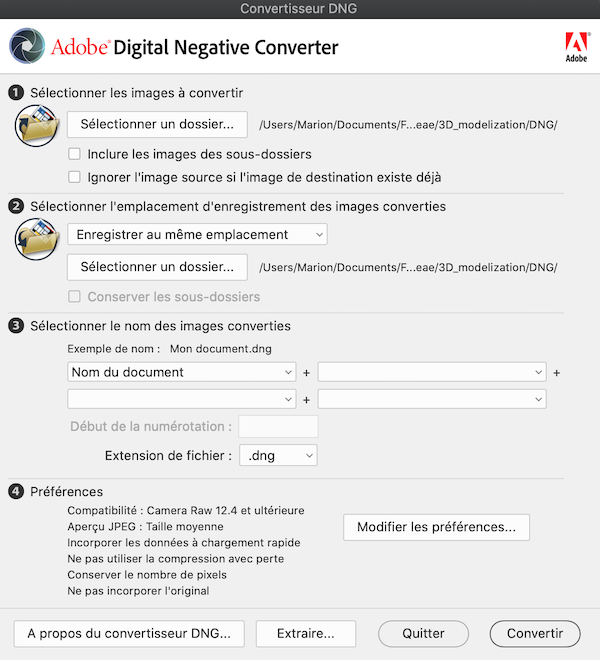
\includegraphics[width=1\textwidth]{Figures/AdobeDNGConverter.png}
  \caption{Convert RAW chart to DNG in Adobe DNG Converter}
  \label{adobe_dng}
\end{subfigure}
\vspace{10pt}
\begin{subfigure}[t]{.45\textwidth}
  \centering
  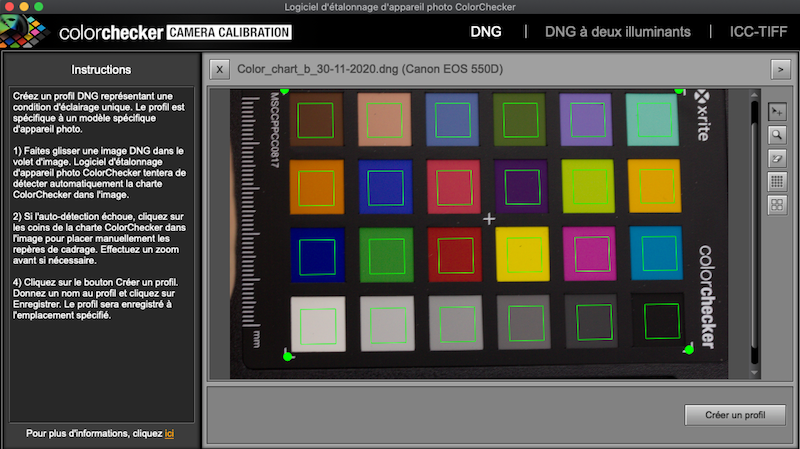
\includegraphics[width=1\textwidth]{Figures/ColorChecker camera cailbration.png}
  \caption{Align grid on chart in ColorChecker Camera Calibration}
  \label{color_checker_camera_calibration}
\end{subfigure}%
\vspace{10pt}
\begin{subfigure}[t]{.45\textwidth}
  \centering
  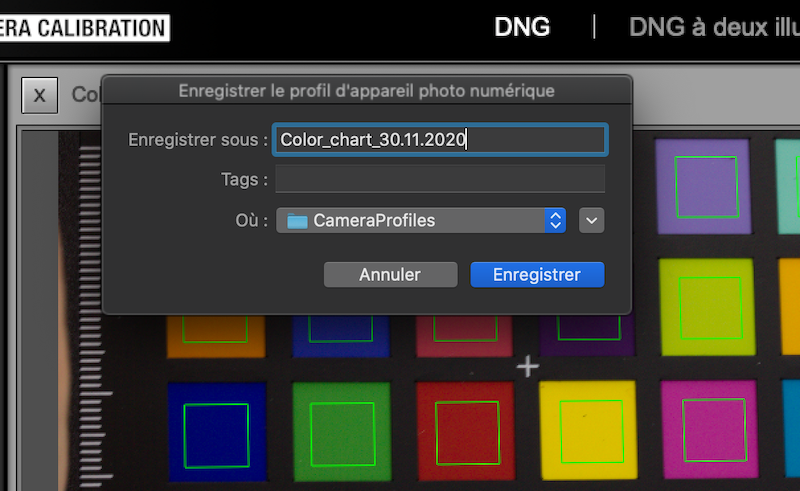
\includegraphics[width=1\textwidth]{Figures/create profile.png}
  \caption{Export the color profile}
  \label{color_checker_profile}
\end{subfigure}
\caption{Manual method for the creation of color calibration profiles from a RAW color chart.}
\label{Manual method}
\end{figure}


\begin{figure}[H]
    \centering
    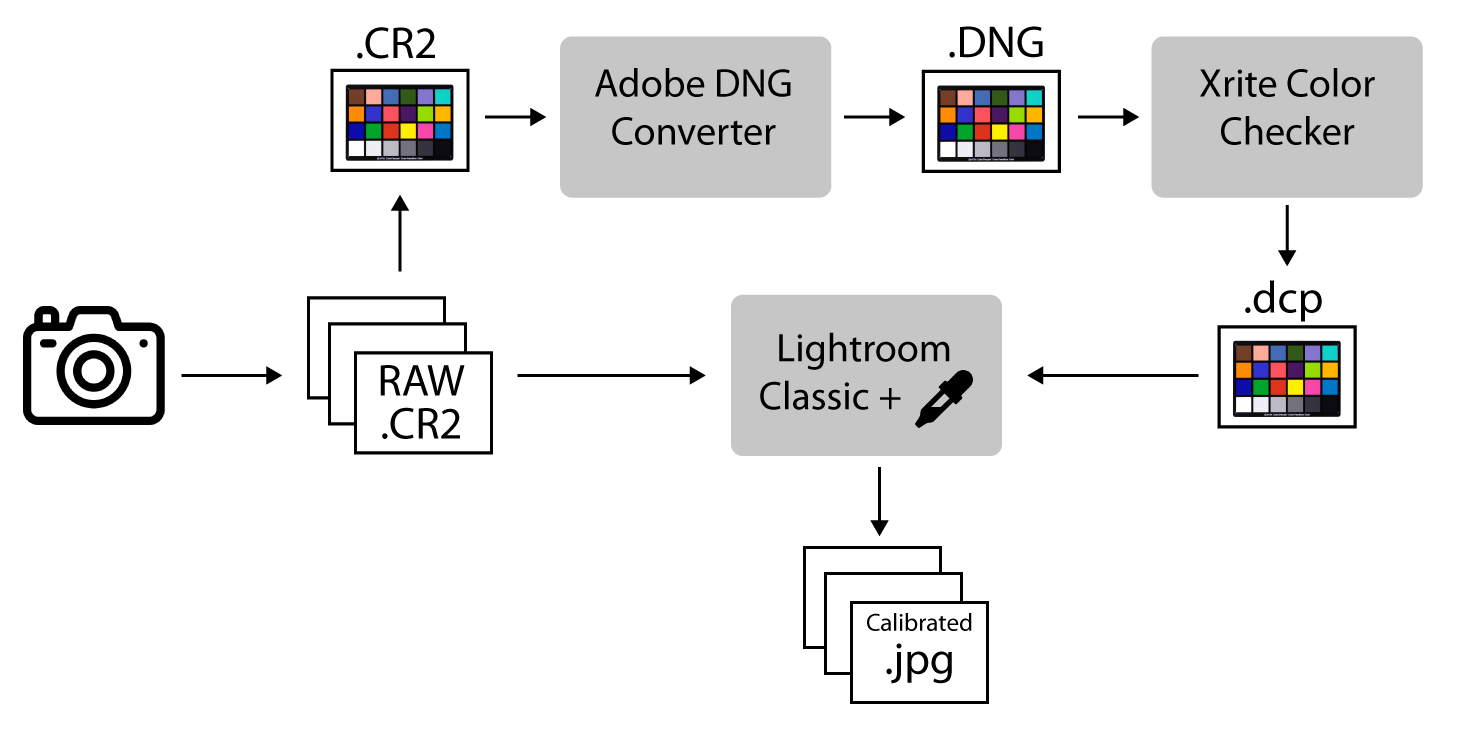
\includegraphics[width=0.8\textwidth]{Figures/manual_method.png}
    \caption{Image color calibration workflow}
    \label{fig:workflow}
\end{figure}



\bigskip
\noindent \textbf{Method 2 : X-Rite Color Checker plug-in installation and automatic creation of color profiles on MacOS}

\begin{enumerate}
    \item Directly in Adobe Lightroom, you can add ColorChecker Camera Calibration as a module to a means of exporting files directly into a color profile.
    \begin{enumerate}
        \item Click on File > Export > \textit{Plug-in Manager} (or \textit{gestionnaire des modules externes} in the left bottom corner)
        \item Click on \textit{Add}
        \item Navigate to \textit{Library} > \textit{Application Support} > \textit{Adobe} > \textit{Lightroom} > \textit{Modules}
        \item Select \textit{XRiteColorCheckerPassport.lrplugin} and then click on \textit{Add Plug-in} and \textit{done}.
        %https://xritephoto.com/ph_product_overview.aspx?ID=1257&Action=Support&SupportID=5927
    \end{enumerate}

    \item Click on the color chart then \textit{File} > \textit{Export} > Choose \textit{Xrite presets} from the drop down menu.
    \item Name your profile then > \textit{Export}
    \item It will go through ColorCheckerCamera calibration to automatically create the profile.
    \item Restart Lightroom as indicated.
\end{enumerate}

\bigskip
\noindent \textbf{Method 3 : X-Rite Color Checker plug-in installation and automatic creation of color profiles on Windows}


\begin{enumerate}
    \item Get the \href{https://xritephoto.com/ph_product_overview.aspx?ID=938&Action=Support&SoftwareID=2030}{Xrite ColorChecker Camera Calibration software} and download the \textit{PC Version}. Save the \textit{CameraCalibrationSetup.exe} in your downloads, for example, and run the program.
    \item If Adobe Lightroom Classic is already installed on your computer, the installation program should proposed you to install the Adobe Photoshop Lightroom plug-in (Figure \ref{color_checker_plug_in_win}). Install it.
    \item Once the plug-in is installed, run Adobe Lightroom Classic and import your color chart (\textit{File} > \textit{Import}).
    \item Click on \textit{File} > \textit{Export} and in the drop-down menu, select \textit{X-Rite Preselection} (Figure \ref{x_rite_preselection}). Name your profile, and click on \textit{Export}.
    \item Restart Lightroom as indicated.
    \item Run the setps 4 and 5 each time you want to create a new color profile witht the color chart.
    
    
\end{enumerate}

\begin{figure}[H]
\centering
  \centering
  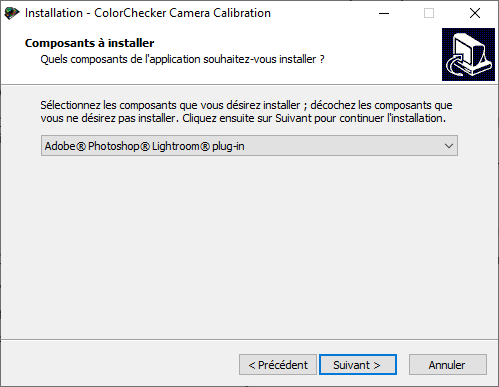
\includegraphics[height=7cm]{Figures/color_checker_plug_in_win.png}
  \caption{Color Checker plug-in for Lightroom installation}
  \label{color_checker_plug_in_win}
\end{figure}%

\begin{figure}[H]
  \centering
  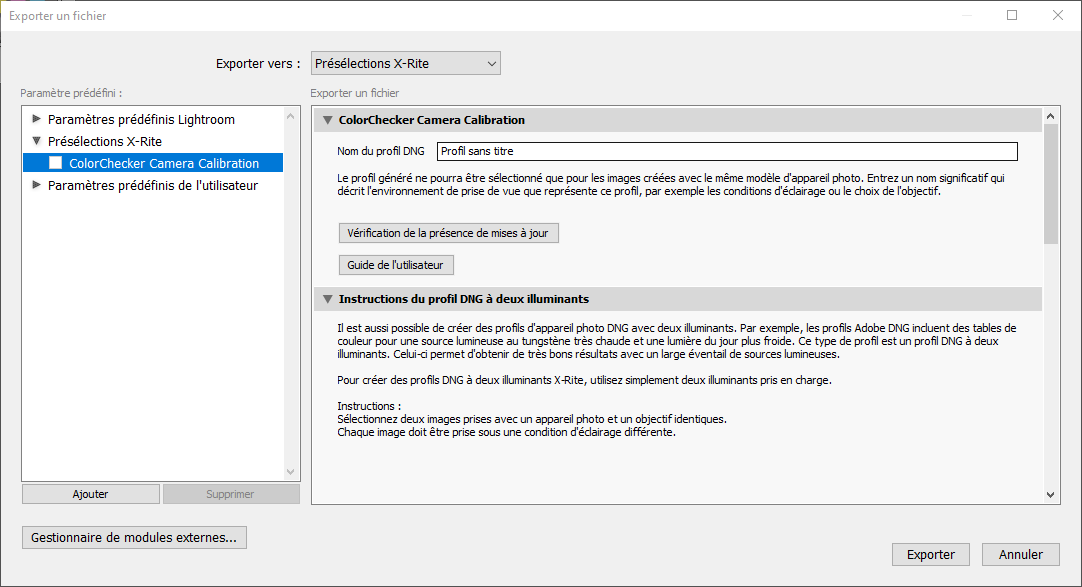
\includegraphics[height=7cm]{Figures/x_rite_preselection.png}
  \caption{Color chart profile exportation}
  \label{x_rite_preselection}
\end{figure}

\subsubsection{Color and illuminance calibration from profiles}

\begin{enumerate}
    %Synchronize Settings is very useful to apply settings to a whole series of images. When viewing a series of images in the main window, or filmstrip, select an image that has the setting that you want to share across to other images. Select all of the other images you want to share the settings with and use the Sync option.
    \item Import your photos in Lightroom Classic. \textit {File} > \textit{Import} then select your folder of RAW photos.
    \item Select the tab \textit{development}.
    \item Select the photo of the chart
    \item Select the color profile corresponding to the color chart you have selected (see Figure \ref{color profile} to manually add a color profile) to calibrate the photo of the chart with its own calibration profile.
    
\begin{figure}[H]
\centering
\begin{subfigure}[t]{0.45\textwidth}
  \centering
  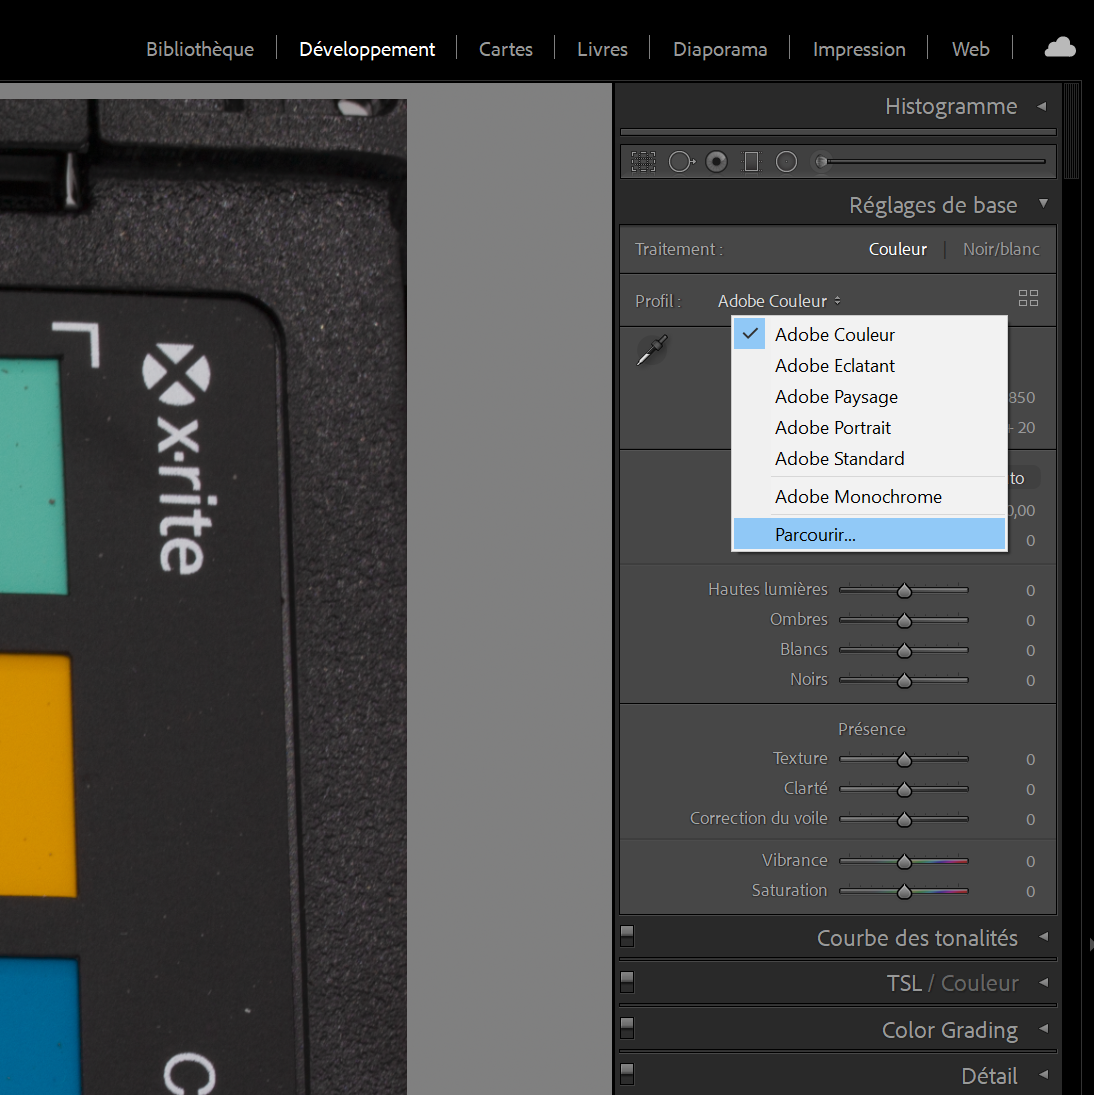
\includegraphics[height=7cm]{Figures/profil_capture_1.png}
  \caption{Add a new color profile}
  \label{add_profile}
\end{subfigure}%
\hspace{10pt}
\begin{subfigure}[t]{0.4\textwidth}
  \centering
  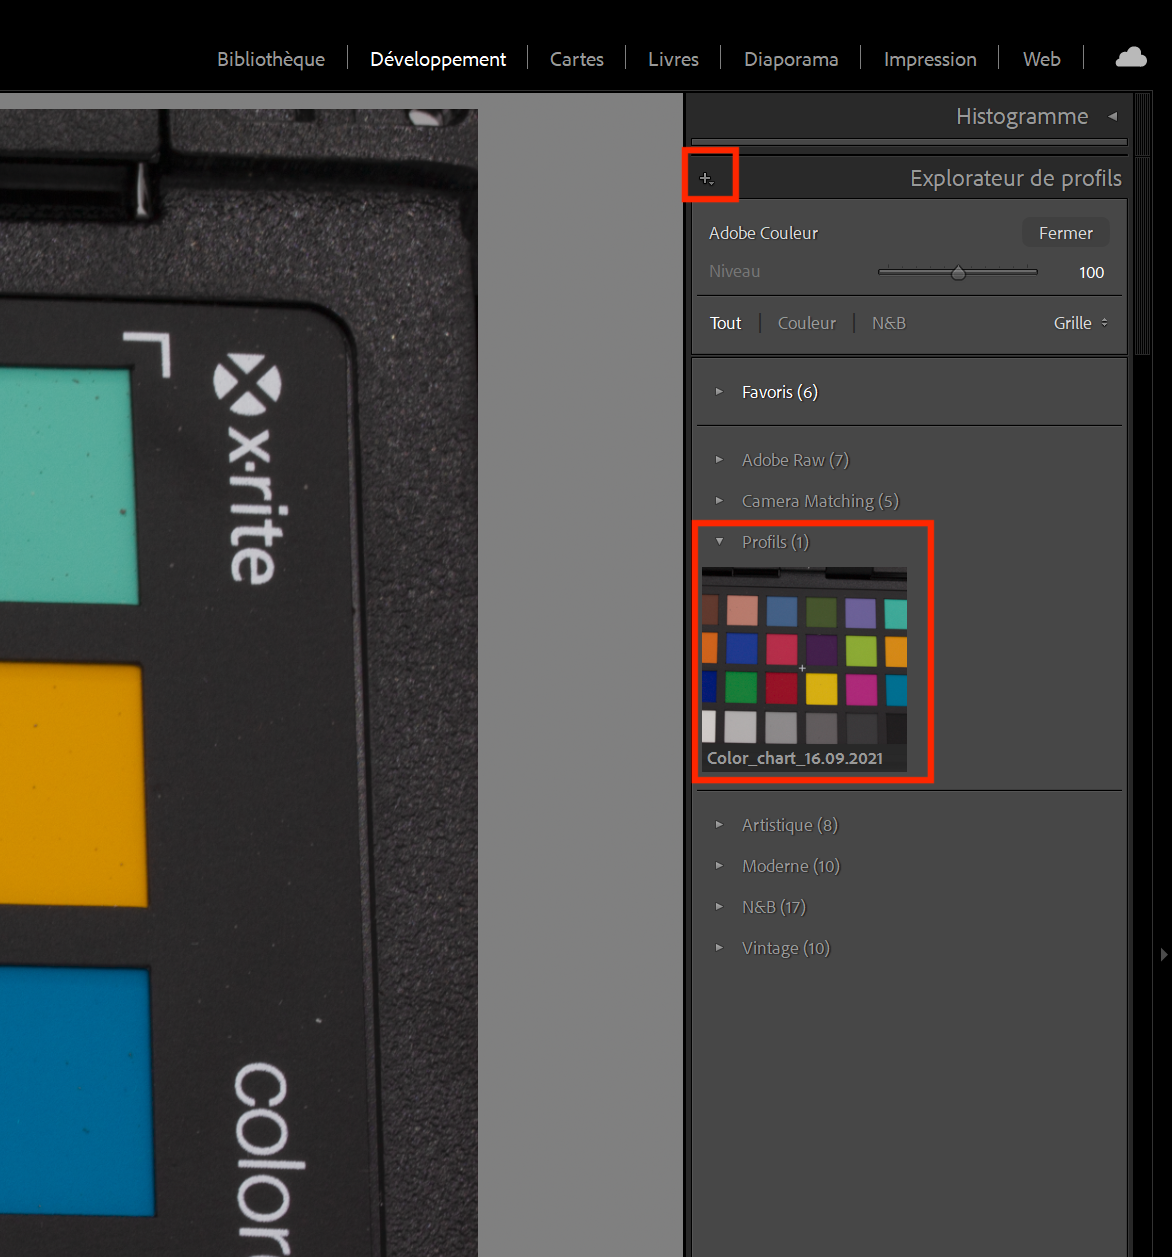
\includegraphics[height=7cm]{Figures/profil_capture_2.png}
  \caption{After adding a profile with the + sign, select it in the list below.}
  \label{settings_synchronize}
\end{subfigure}
\caption{Manually add a new color profile corresponding to the .dcp file created from Adobe DNG converter and Xrite Color Checker}
\label{color profile}
\end{figure}
    
    \item Use the eyedropper over the 75\% gray scale (the last one before the black chip on the color chart, see Figure \ref{fig:xrite_description}). Do not click on the photo with the eye dropper, only hover over the photo.
    \item Select the exposition setting, and adjust the values the eyedropper indicates of the gray scale using the exposition setting to obtain the RGB values of the closest values to 0.33 0.33 0.33 (corresponding to 85/255 for each of the red, blue, and green class). The illuminance is now adjusted in addition to the color calibration, but only on the chart.
    \item To apply the modifications we just did to all the photos, select all the photos (Cmd+A or Ctrl+A), and make sure that the one for which you made changes is highlighted (in white compared to light gray for the other ones selected) (see Figure \ref{fig:synchronize}). Check the profiles and exposure boxes before synchronizing to all the other photos.
    \item Click on the button \textit{synchronize}.
\end{enumerate}

%The gray scale from left to right:
%WHITE = 243 243 243 = 5%
%NEUTRAL 8 = 200 200 200 = 26%
%NEUTRAL 65 = 160 160 160 = 44%
%NEUTRAL 5 = 122 122 121 = 62%
%NEUTRAL 35 = 85 85 85 = 75%
%BLACK = 52 52 52 = 86%



\begin{figure}[H]
    \centering
    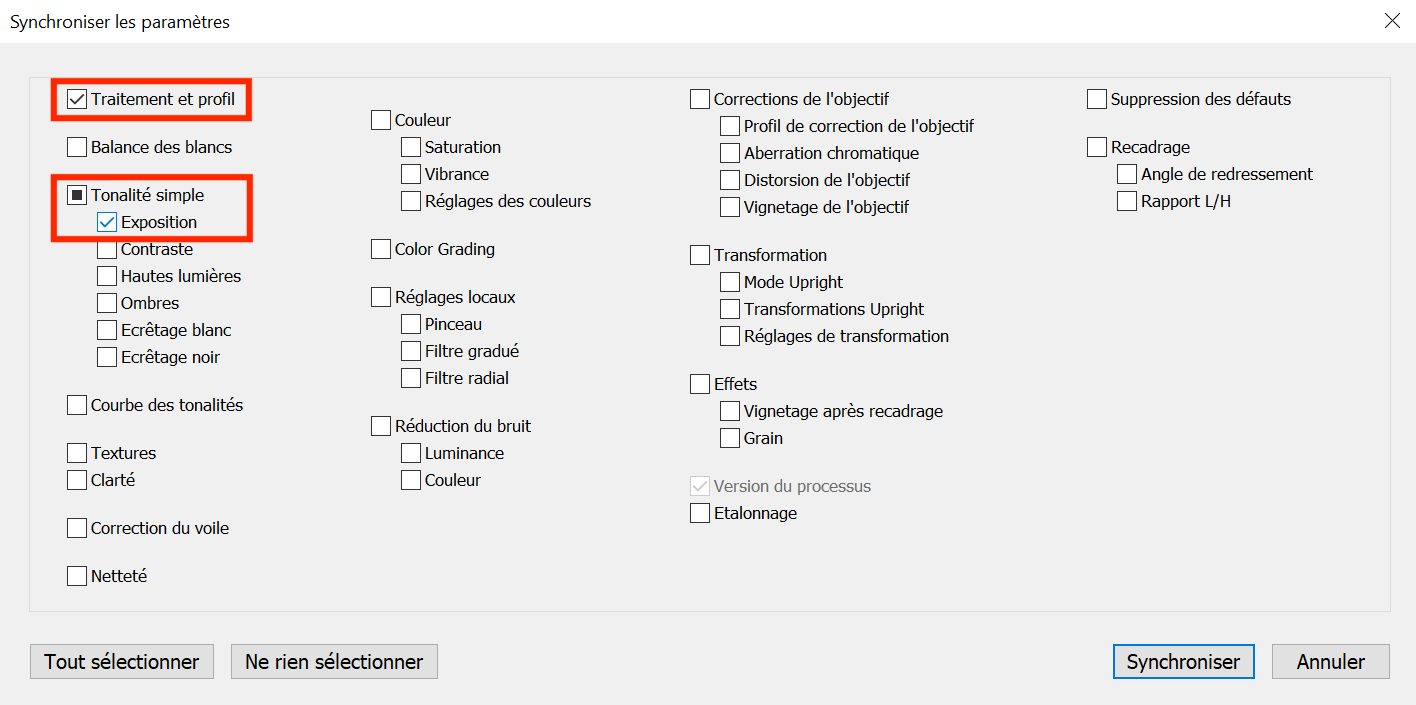
\includegraphics[width=1\linewidth]{Figures/synchronize_capture.png}
    \caption{Synchronize your settings made to the photo of the chart to all the other photos and check the two categories you modified (color profile and exposure).}
    \label{fig:synchronize}
\end{figure}



\subsubsection{Export calibrated files to jpg format}

\begin{enumerate}
    \item Select all the photos you need to export or all of them (cmd+A or windows+A)
    \item Click on \textit{File} > \textit{Export}
    \item You can create presets that you will only need to create once to always export the same way in Adobe Lightroom (example Figure \ref{export_parameters}), and add personalized file names such as \_color\_calibrated at the end of each .jpg file (see also for that Figure \ref{export_parameters}).
    \item In their own folder, you can then sort the calibrated photos for color and exposure per chunks (easily distinguishable by the separation created by a photo of the label).
\end{enumerate}




\begin{figure}[H]
    \centering
    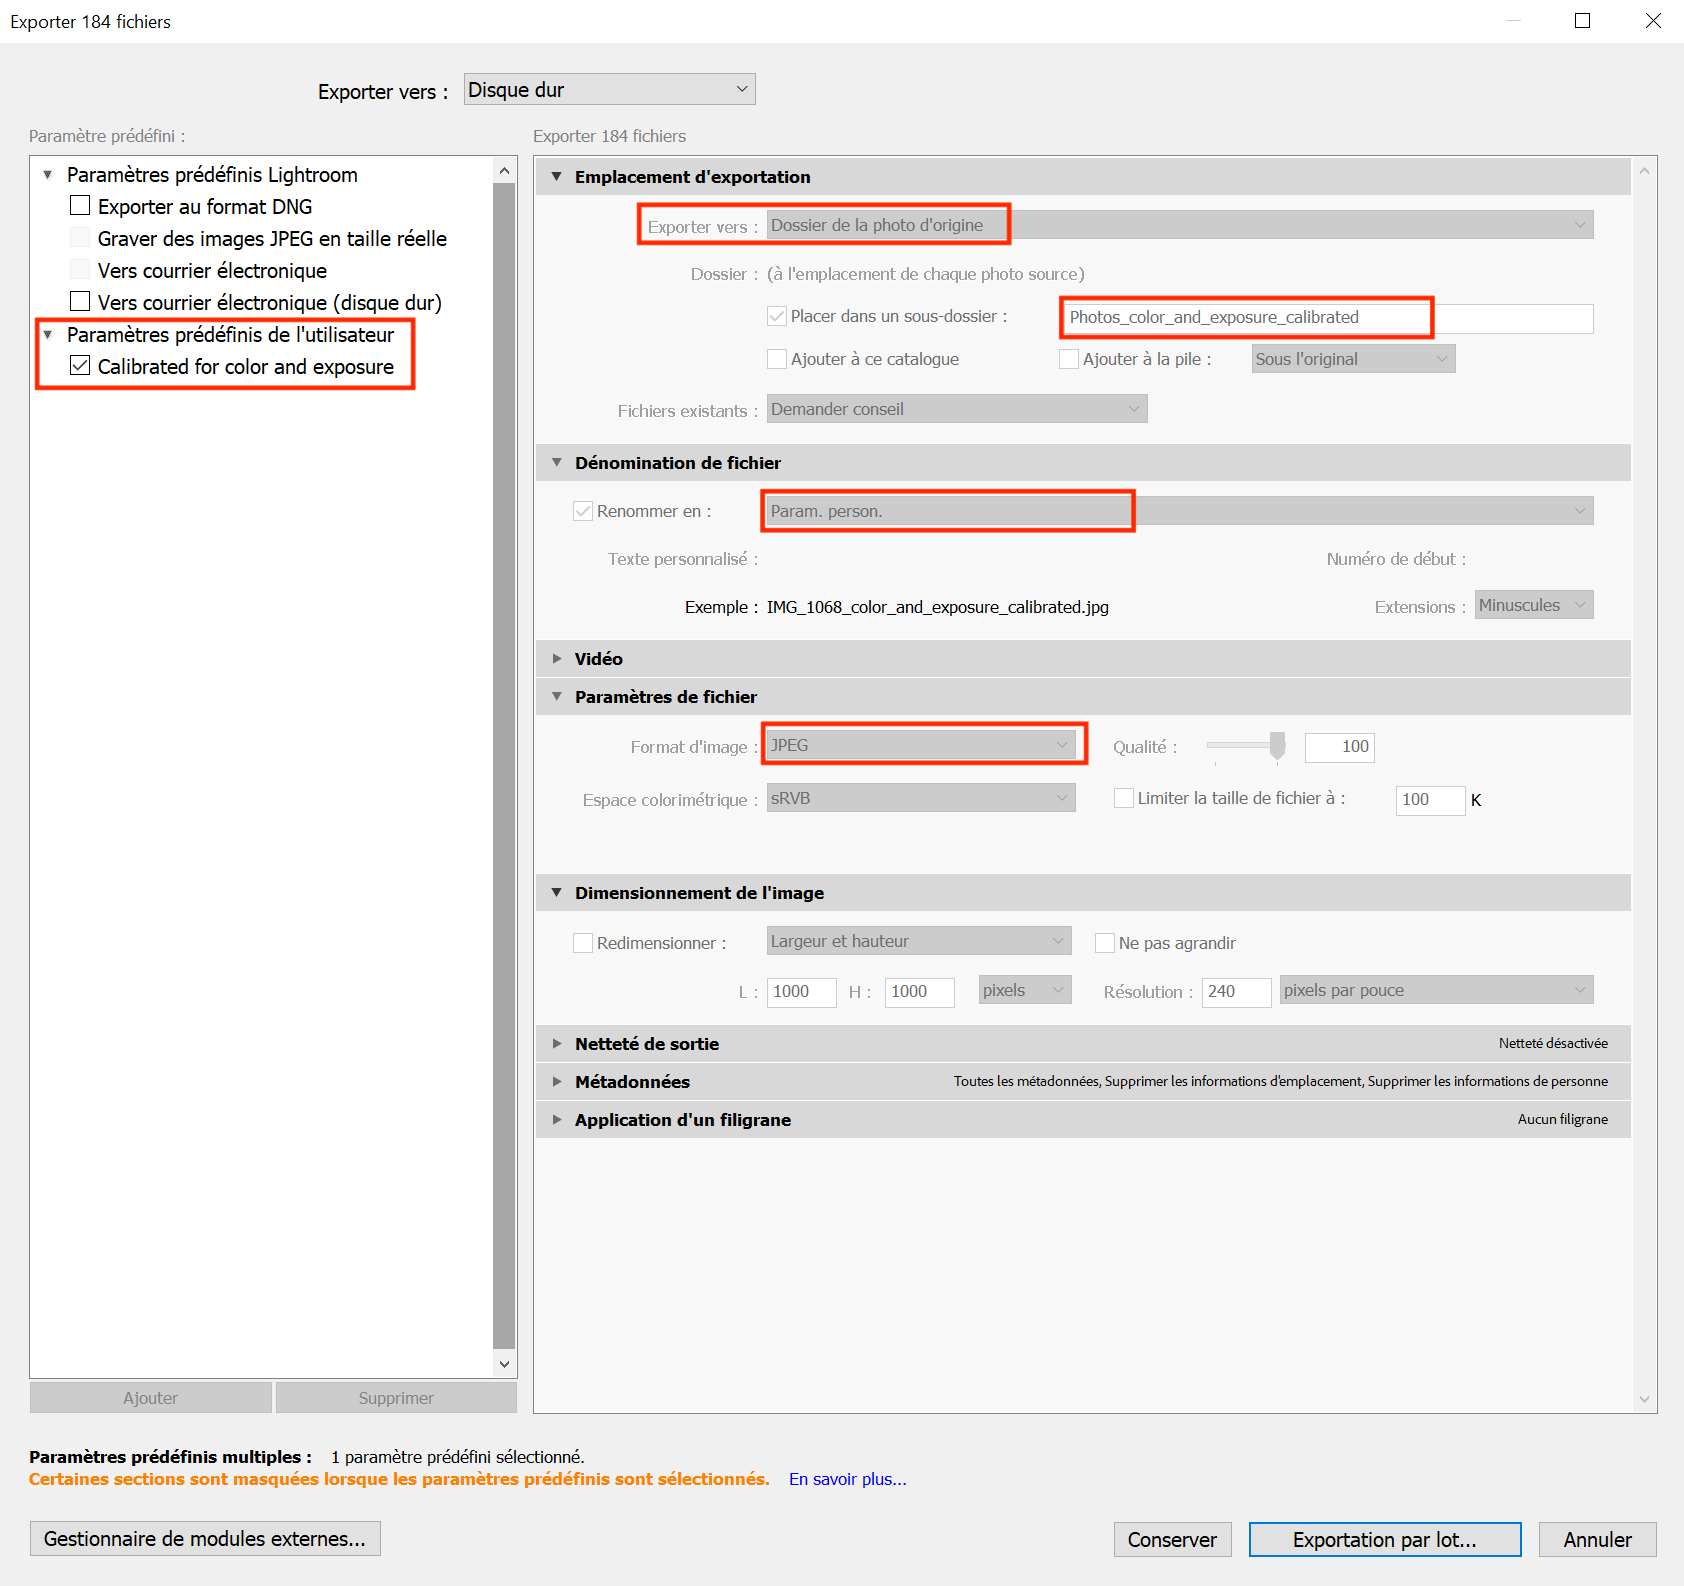
\includegraphics[width=0.9\textwidth]{Figures/export_capture_1.png}
    \caption{You can export using your own personalized parameters and then export in batch your selection in a specific folder within your folder of uncalibrated photos for easy access. This method can thus work for any folder of uncalibrated photos.}
    \label{export_parameters}
\end{figure}




\newpage
\section{3D model reconstruction in Agisoft Metashape}

Software you will need :

\begin{figure}[H]
\centering
\begin{subfigure}{.3\textwidth}
  \centering
  
\includegraphics[width=0.3\textwidth]{Figures/logo_photoshop.png}
  \caption{Optionally, Adobe Photoshop}
  \label{}
\end{subfigure}%
\begin{subfigure}{.3\textwidth}
  \centering
  
\includegraphics[width=0.4\textwidth]{Figures/logo_metashape.jpeg}
  \caption{Agisoft Metashape}
  \label{}
\end{subfigure}
\caption{Softwares for 3D reconstruction}
\label{}
\end{figure}





\subsection{Download Agisoft Metashape}

Download the Agisoft Metashape professional edition software \href{https://www.agisoft.com/downloads/installer/}{here}. Make sure that your computer fills the \href{https://www.agisoft.com/downloads/system-requirements/}{minimum system requirements}.
The standard edition doesn't allow the use of the scale option that we will need to add a scale on our models.

\subsection{Initial tweaks}

Agisoft Metashape can use graphic cards at certain steps of the model construction such as image matching and depth maps calculation. To enable the use of the graphic hardware (GPU):

\begin{itemize}
    \item Select Preferences command from the Tools menu.
    \item In Preferences dialog select GPU tab.
    \item Select available GPU devices in GPU tab of the Preferences window
\end{itemize}

This step has to be done only once.



This protocol has been elaborated using the version 1.7.1 of Agisoft Metashape. The latest version of Metashape is now version 1.8.2, but we still made the following changes. In order to obtain accurate thin structures, such as petal margin, and avoid holes in your mesh in Agisoft Metashape 1.5.x or later (up to our knowlege) you will need to activate ONCE the \textit{Visibility consistent mesh} function in \textit{Tools > Preferences > Advanced >Tweaks}, then \textit{Add} and fill in \textit{Parameters} with \textit{BuildModel/tvl1\_mesh} and select the value as \textit{False} (figure \ref{metashape_tweaks}). Additionally, to use the anterior version of the depth maps generation process, add ONCE the tweak : \textit{BuildDepthMaps/pm\_enable} and set the value to \textit{False} (figure \ref{metashape_tweaks}).


\begin{figure}[H]
\centering
\begin{subfigure}{.45\textwidth}
  \centering
  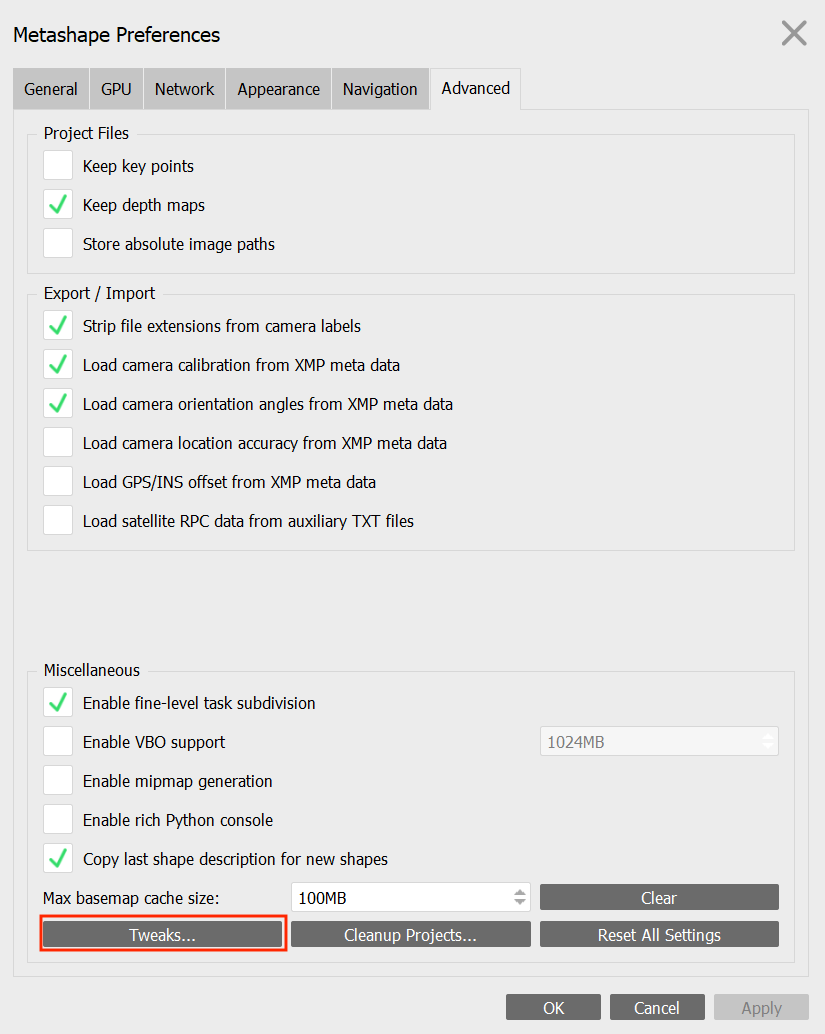
\includegraphics[width=1\textwidth]{Figures/Metashape_tweaks_1.png}
  \caption{}
  \label{}
\end{subfigure}%
\hspace{0.5cm}
\begin{subfigure}{.45\textwidth}
  \centering
  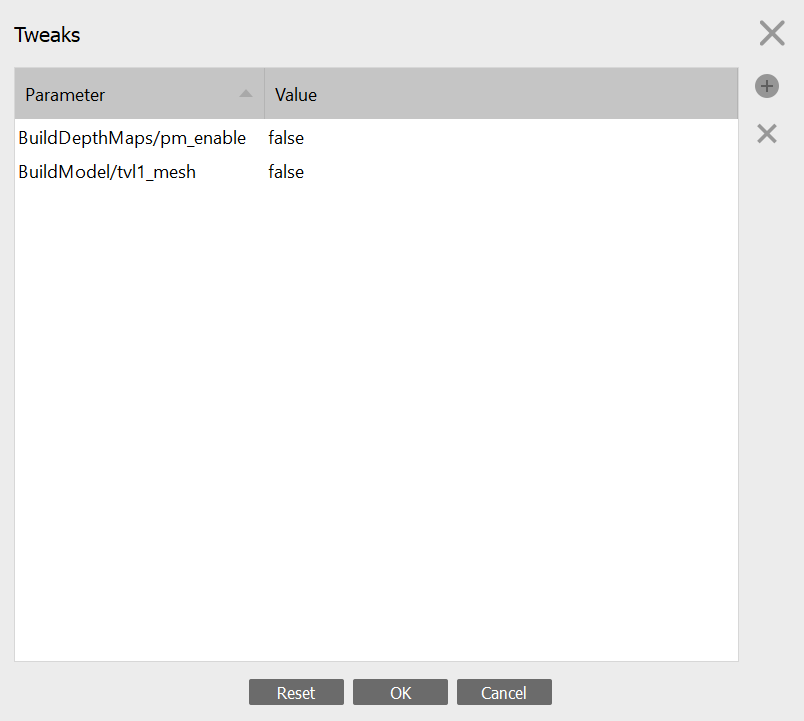
\includegraphics[width=1\textwidth]{Figures/Metashape_tweaks_2.png}
  \caption{}
  \label{}
\end{subfigure}
\caption{Tweaks settings in Metashape}
\label{}
\end{figure}


\subsection{Overview of the model building pipeline}

To build a model, we need to do the following steps: 1) Import the calibrated photos, 2) apply masks to remove background on the photos, 3) align the cameras, 4) calculate depth maps, 5) build the 3D model (mesh), and 6) reconstruct the final texture (model color). There could be different approaches for each of the steps and options will be given below.

One important note is whether all the pictures (cameras) are aligned simultaneously of if it is necessary to proceed by groups of pictures that correspond to each flower positions. The first approach is quicker and normally results in more accurate models. However, it does not work all the times. We recommend to try it first and if it fails to use the alternative approach, which is to divide the pictures in different "chunks" that will create partial 3D models.


\subsection{Photo importation}

Go to \textit{Workflow}, click on \textit{Add Photos}, and click \textit{Open}. Once the photos are imported, they are in a single "chunk", which is a group of photos.

To try to align all the photos simultaneously (ideal approach), you need to arrange them in "camera groups", where each camera group contains all pictures taken with the same flower orientation. Once this is done, you can add the first photo of each set of photos representing the label, and right click on this photo and select \textit{disable cameras}. This allows you to not take it into account while reconstructing the model, but to keep all the information about the flower in your Metashape project.


\subsection{Mask application}

Masks represent selected areas that are excluded from the feature detection procedure when applied to key points detection. When several keypoints are detected as the same point (matched as projections of the same 3D point on different photos), then it is considered as a tie point. If masks are applied to tie points, then if a key point is masked in at least one image, it will not be considered. You can thus use a single or just a few masks with the second method (apply masks to tie points). It is however possible to automatically apply masks on each photo to better constrain key point detection (apply masks to keypoints). Using masks helps in removing points to be detected in the background during image alignment procedure.
You can see examples \href{https://agisoft.freshdesk.com/support/solutions/articles/31000158967-aligning-turntable-photos-with-background-suppression-from-single-mask-in-agisoft-metashape}{here} on the Agisoft helpdesk portal.

\noindent \textbf{Step-by-step mask application workflow}

\begin{enumerate} 
    \item Duplicate one of your photos, and fill it in black in any image manipulation software, and rename it as \textit{background.jpg}. You can also take a picture of the lightbox without your flower just before starting to shoot and use this image as background. This sometimes work better.
    \item Right click on a photo in one of your chunk in your Metashape project.
    \item Click on \textit{Masks}, \textit{Import Masks} and in the box that appears select method "From Background", operation  \textit{Replacement}.
    \item Enter the same name as the name of your background you just saved.
    \item Depending on the flower, the value for \textit{Tolerance} can vary between approximately 40 and 60. For some pale flowers you may need a lower tolerance value (e.g. 30).
    \item Test different values of tolerance on a single photo first, but when you have a value that is satisfactory (that create a masks with the border of the flower well defined) you can select \textit{Apply to entire workspace}
    \item Click OK
    \item This will automatically produce masks around the flowers for all the photos in all your chunks. This is why we need a contrasting white background behind the flower.
    \item Check for masks that need touch ups (next section).
\end{enumerate}


\begin{figure}[H]
\centering
\begin{subfigure}[t]{.45\textwidth}
  \centering
  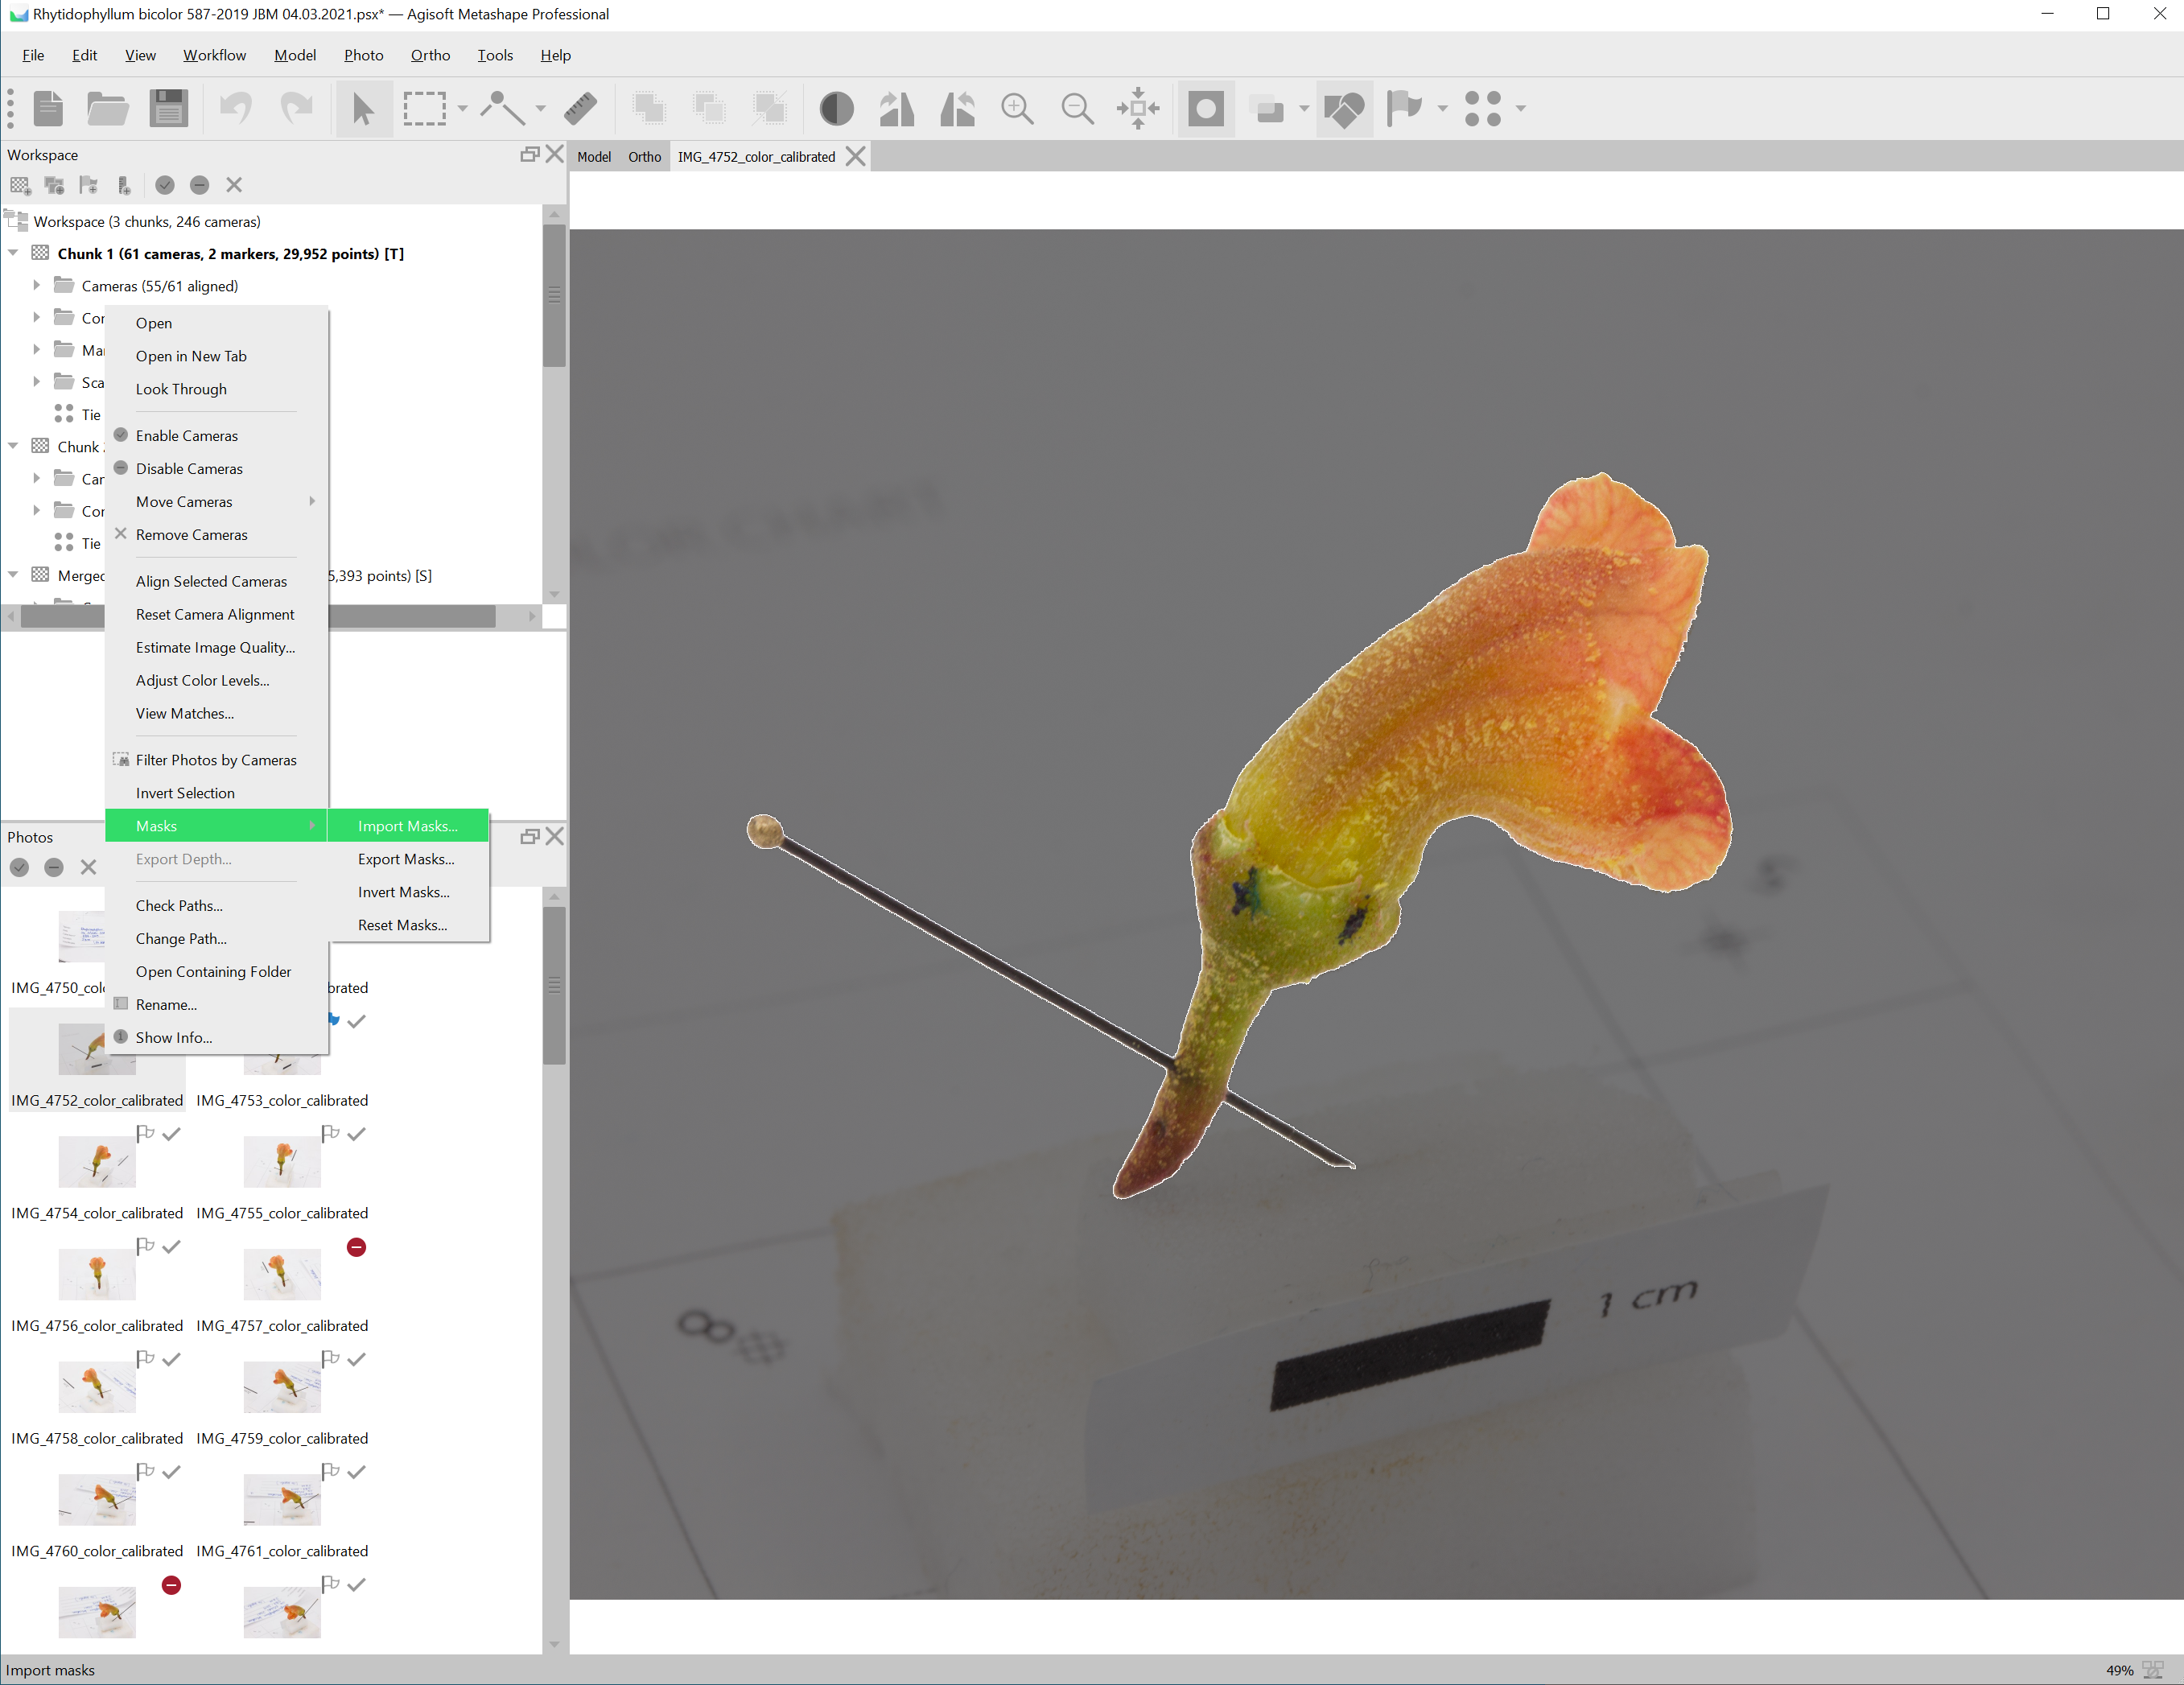
\includegraphics[width=1\textwidth]{Figures/Metashape_mask_right_click.png}
  \caption{Right click on an image to select a mask to import.}
  \label{}
\end{subfigure}%
\hspace{0.5cm}
\begin{subfigure}[t]{.45\textwidth}
  \centering
  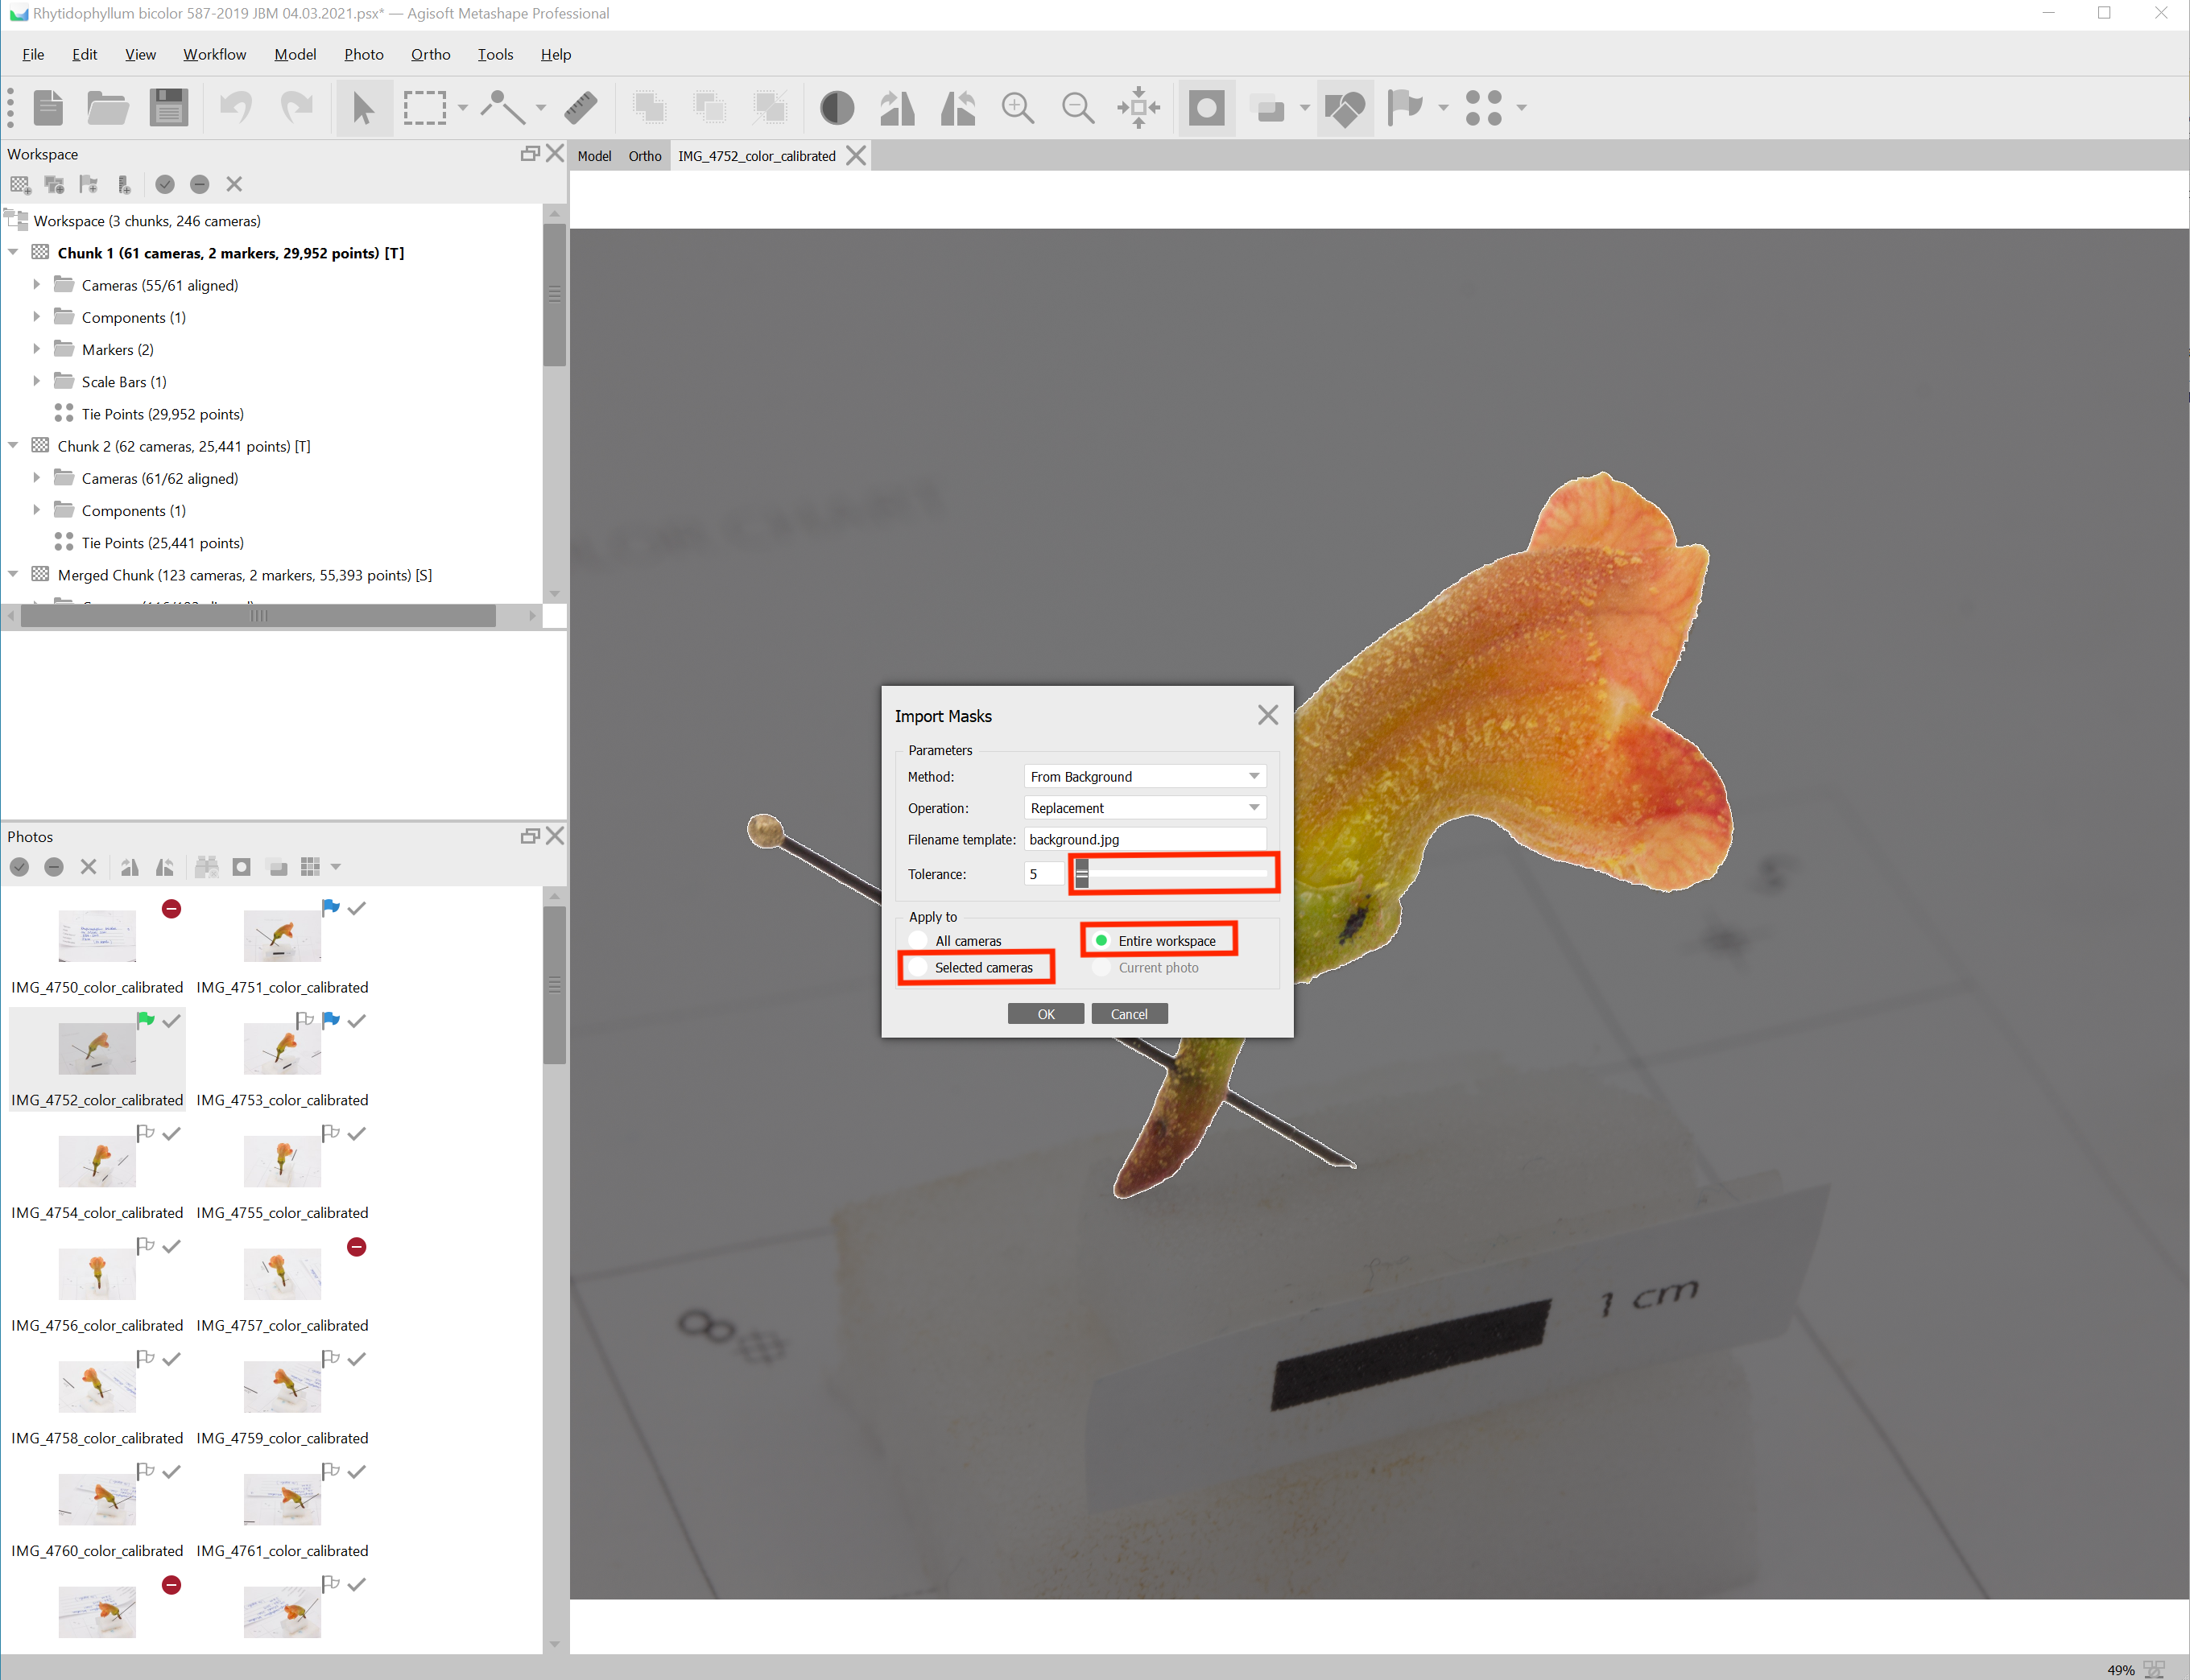
\includegraphics[width=1\textwidth]{Figures/Metashape_masks_tolerance.png}
  \caption{Import mask from a black image \textit{background.jpg}, and select a tolerance value, to test on the selected camera (the image you right-clicked on). If the automatic mask is automatically well adjusted around the flower shape (darker gray around the flower), then apply to entire workspace (all the images).}
  \label{}
\end{subfigure}
\caption{Apply masks to images in Metashape.}
\label{}
\end{figure}


\bigskip
\noindent \textbf{Alternative masking method using Adobe Photoshop}
It is also possible to use Adobe Photoshop to apply masks. We did not find particular improvements compared to the Agisoft Metashape approach.
    \begin{enumerate}
        \item Go to the file containing the pictures of chunk 1. Copy and paste this file, naming it accordingly (e.g. \textit{Chunk1-Background}).
        \item Go to Adobe Photoshop version 19.1 and up.
        \item Make a copy of all of the photos you’ll be using and place them in a new folder labeled \textit{Chunk1-masks}.
        \item Then, you will need to create ONCE a Photoshop action, that will be subsequently reused (see figures below) :
        
%SOURCE
%https://bischrob.github.io/Automatic-Background-Removal-for-Photogrammetry/



\begin{figure}[H]
\centering
\begin{subfigure}[t]{.45\linewidth} % >>> [t] -> helps aligning subfigures according to the image not the text
  \centering
  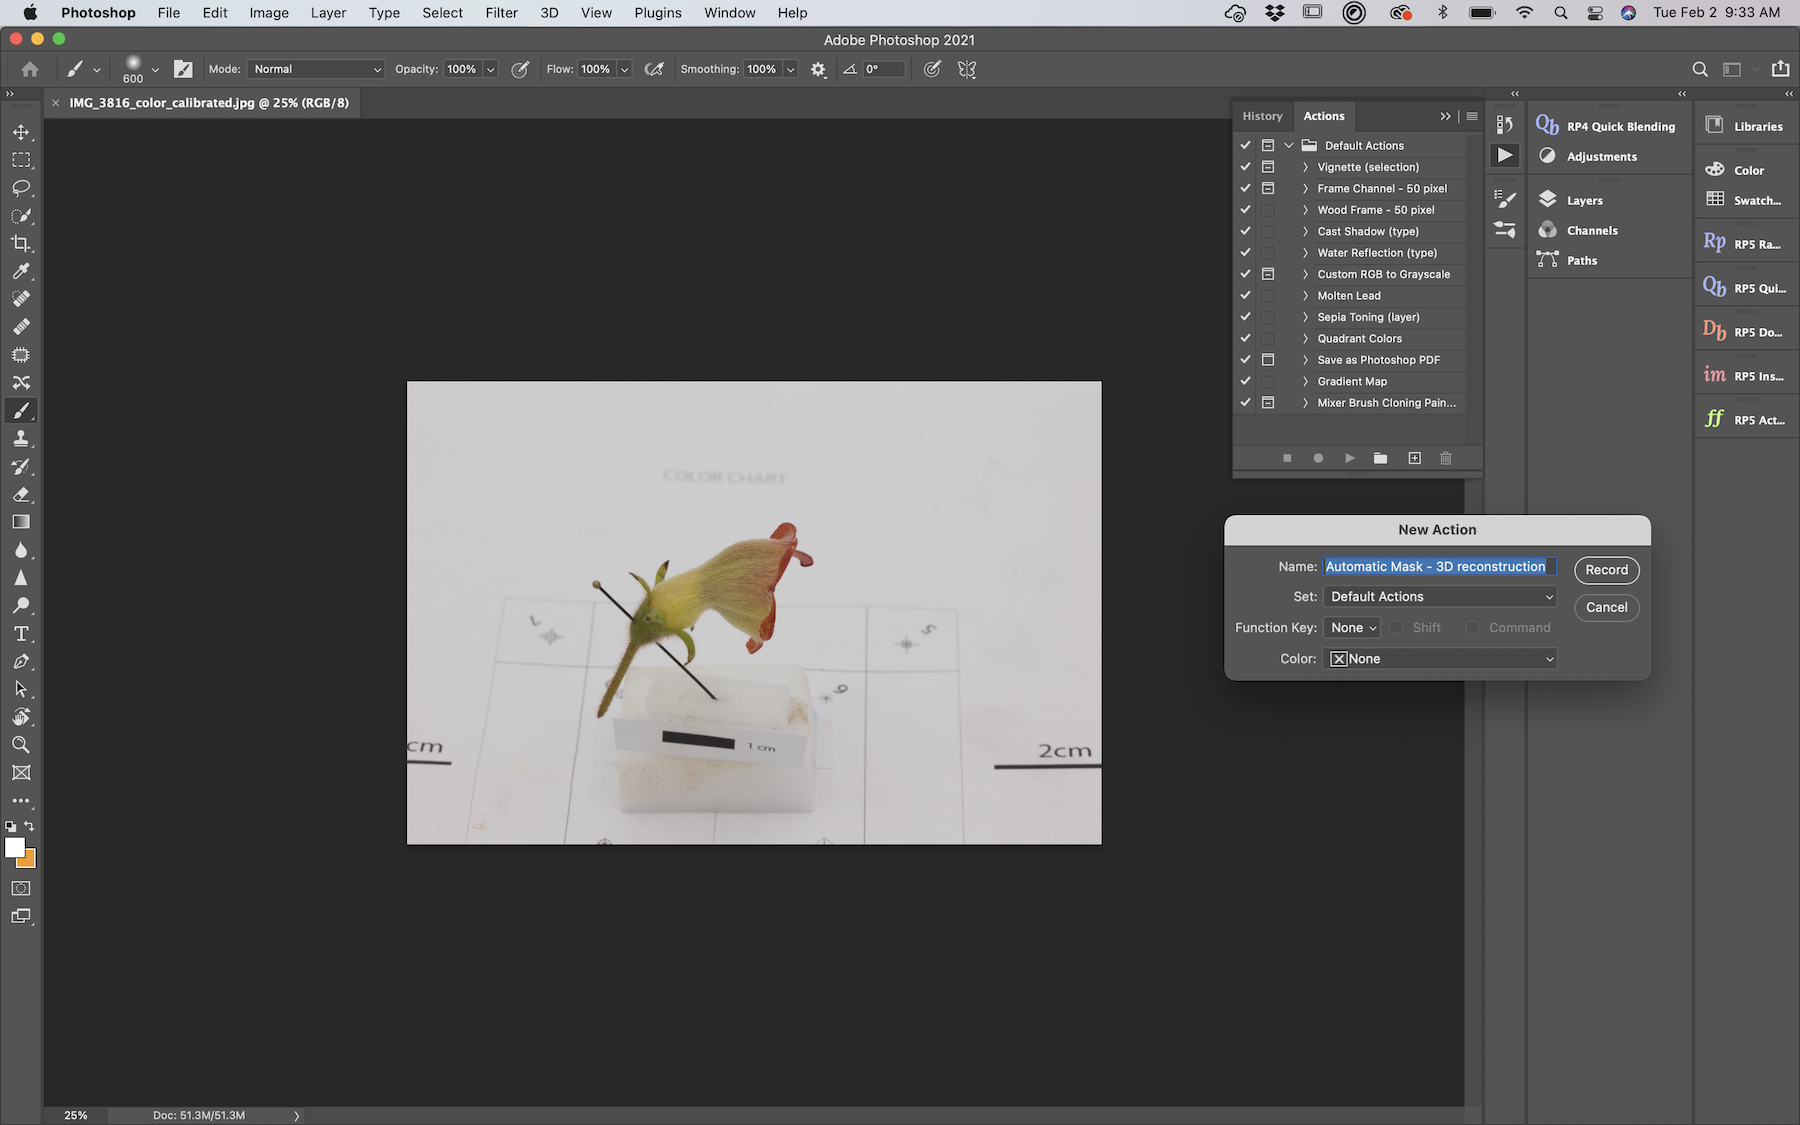
\includegraphics[width=1\linewidth]{Figures/mask_1.png}
  \caption{Record a new action called \textit{Automatic Mask - 3D reconstruction}}
  \label{}
\end{subfigure} \hspace{10pt}%
\begin{subfigure}[t]{.45\linewidth}
  \centering
  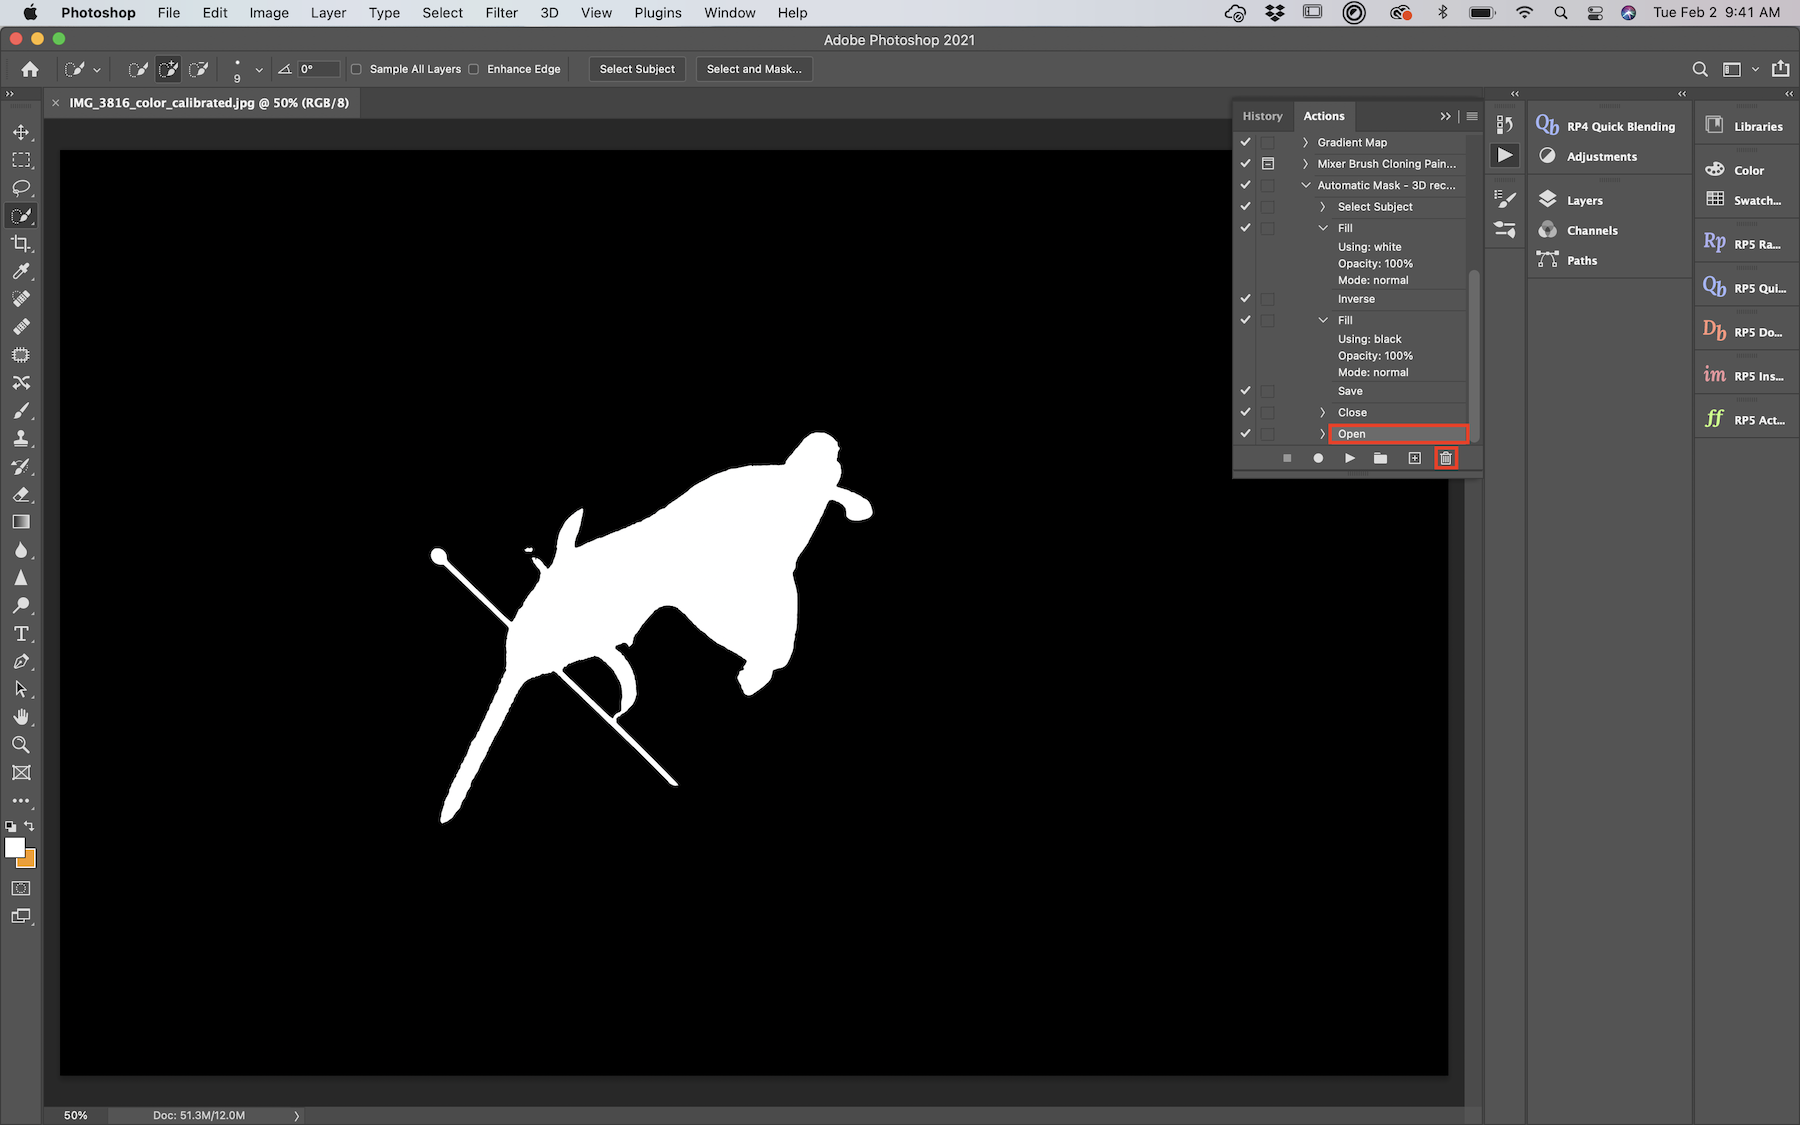
\includegraphics[width=1\linewidth]{Figures/mask_2.png}
  \caption{When you reopen your photo, don't forget to remove this extra task in your action.}
  \label{}
\end{subfigure}
\vspace{10pt}
\begin{subfigure}[t]{.45\linewidth}
  \centering
  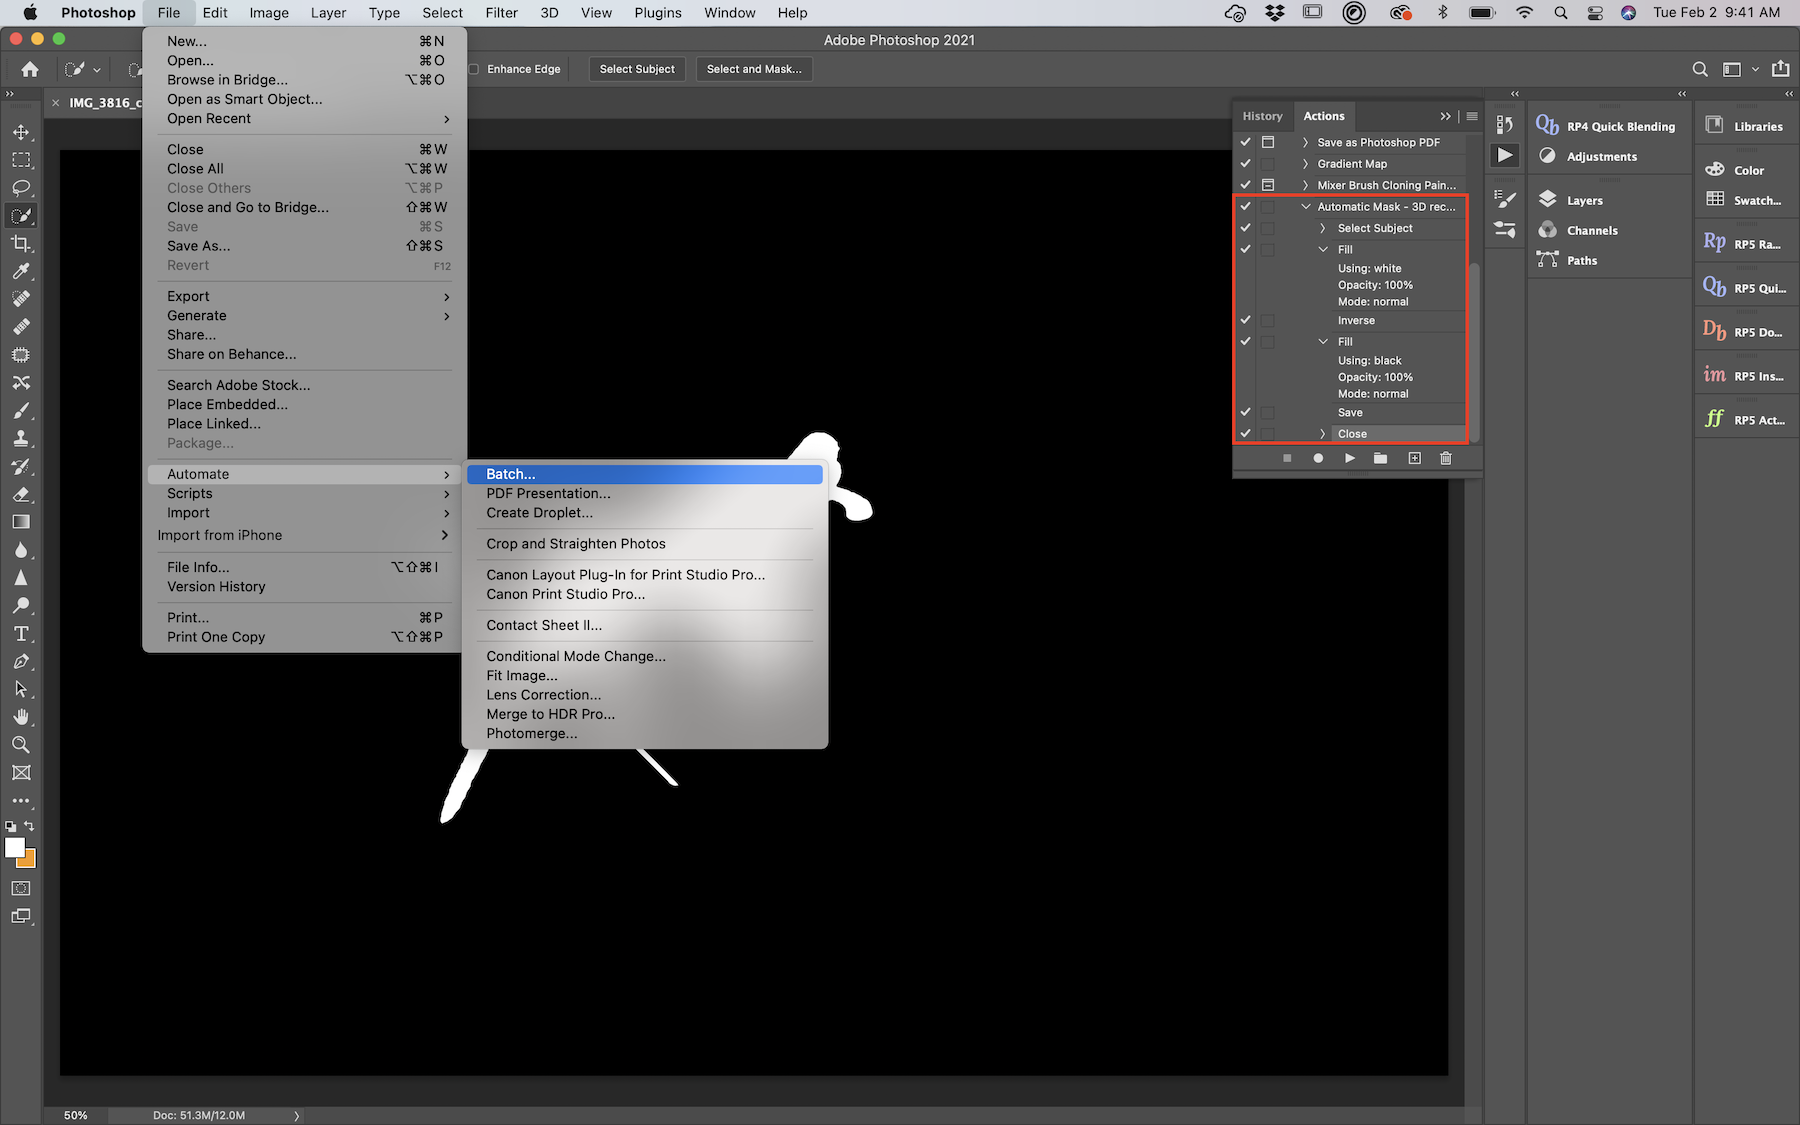
\includegraphics[width=1\linewidth]{Figures/mask_3.png}
  \caption{The action should include \textit{Select Subject, Fill, Inverse, Fill, Save, Close}, and you can batch process this action to a specific folder of copied photos to create masks.}
  \label{}
\end{subfigure}\hspace{10pt}%
\begin{subfigure}[t]{.45\linewidth}
  \centering
  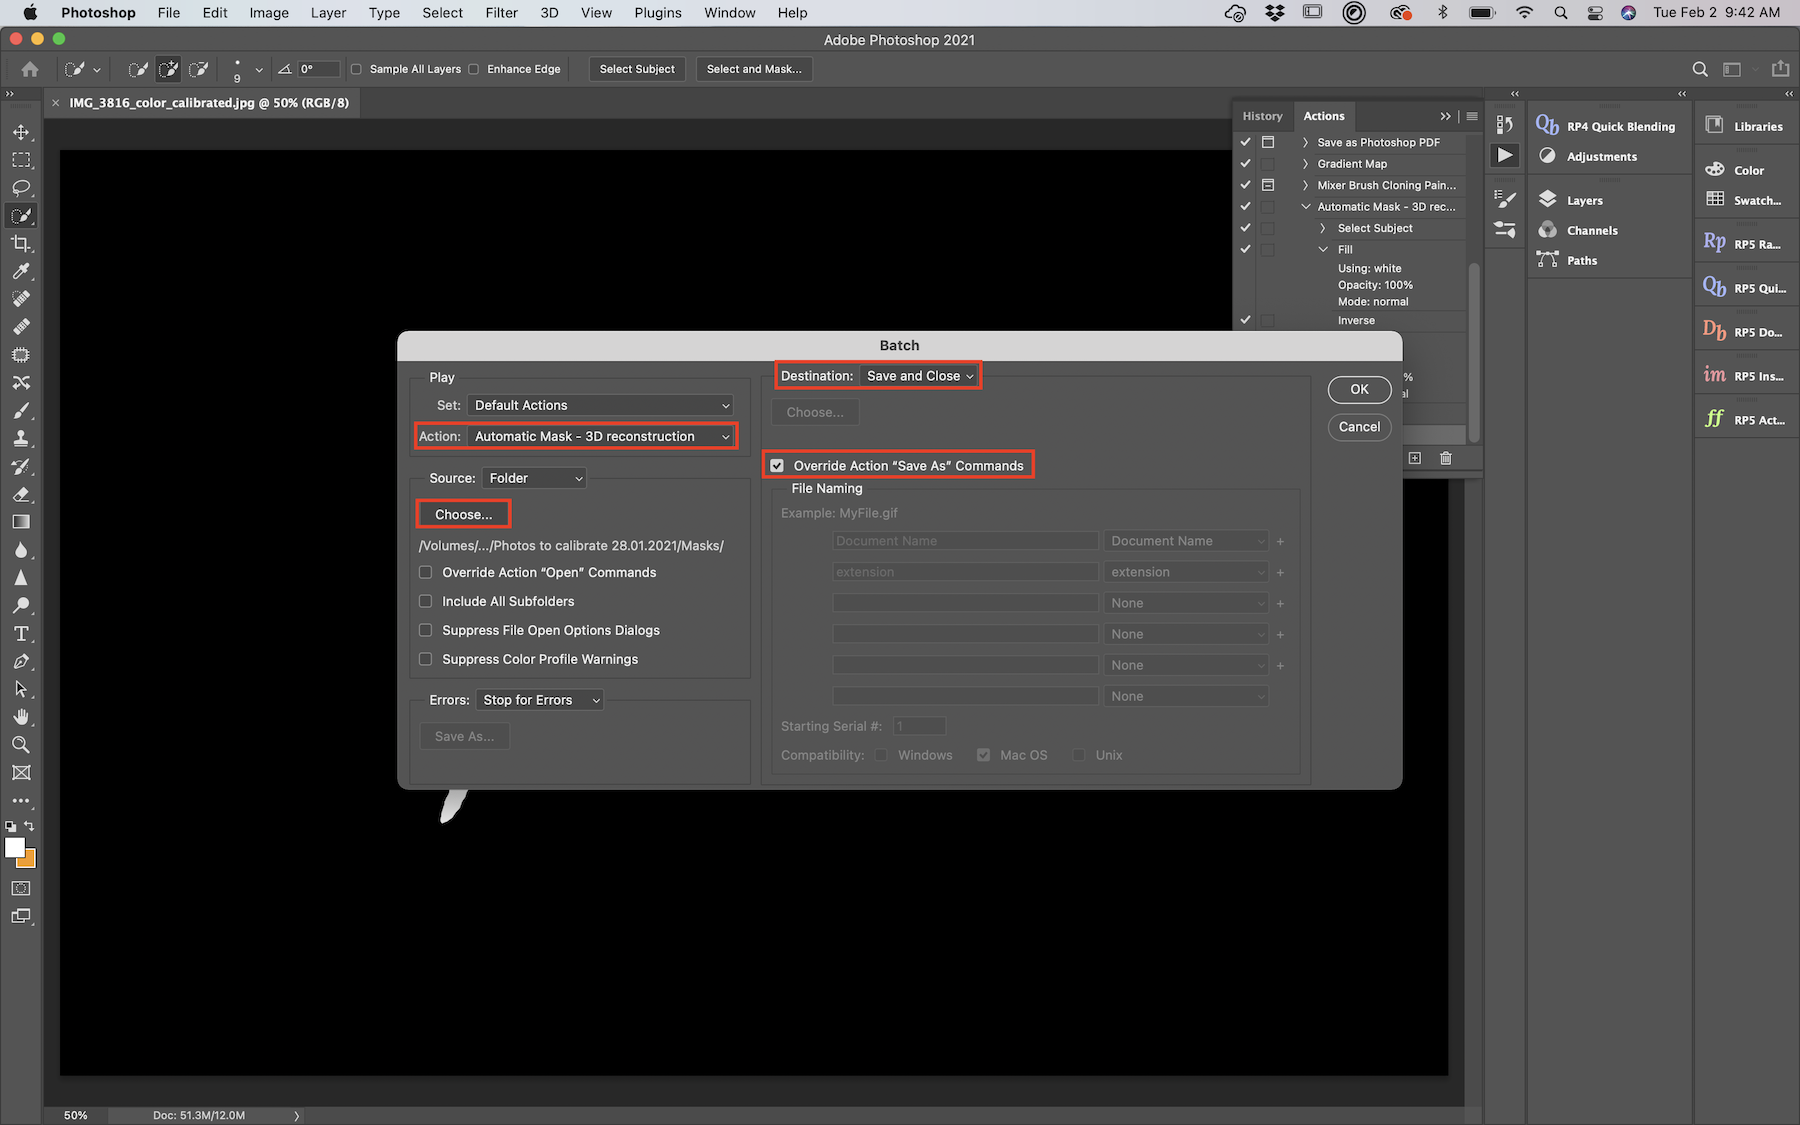
\includegraphics[width=1\linewidth]{Figures/mask_4.png}
  \caption{Apply the action to the folder of copied photos called \textit{Chunk1-masks}.}
  \label{}
\end{subfigure}
  \caption{Create automatic masks using Adobe Photoshop}

\end{figure}


            \item Now you should have tranformed all your copied photos into masks, with the foreground object in white, and the background in black.
            \item Go to Agisoft Metashape and right click on the first camera (photo) of chunk 1. Click on\textit{ Masks > Import Masks} and in the box that appears select method \textit{From file}, operation \textit{Replacement}. In \textit{Filename Template} use \textit{ {filename}.jpg}. Select \textit{Apply to all cameras} and then click \textit{OK}.
            \item Check the masks for touch ups.
            \end{enumerate}
%pour 808 photos -> 25min (sur un très bon ordi).
%pour 206 photos -> 6min
%donc environ 35 photos la minute

% \begin{tcolorbox}[width=\linewidth, colback=mygray,title=Suggestion for the Joly Lab,colframe=lightgray]
% For example, on a MacBook pro (2016), this process converted 35 photos per minute.
% \end{tcolorbox}



\subsection{Masks touch ups}

The automatic application of masks at the previous steps is sometimes not entirely satisfactory for all photos. It is possible to add or remove parts of masks using the selection tool and the add/remove/invert buttons (Figure \ref{tools_masks}).
You can then use the selection tools to select areas that are not the flower and add the selection to the mask (Figure \ref{tools_masks}). You also remove the scale and the entomological pin at this step.
Additionally, you can invert the selection, or remove the selected areas from the mask with the icons on the right hand side of the add to mask icon.



\begin{figure}[H]
  \centering
  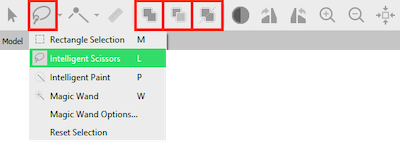
\includegraphics[width=0.5\textwidth]{Figures/tools_masks.png}
  \caption{Selection tools and add selection to mask tool}
  \label{tools_masks}
\end{figure}


%FIGURE of pieces of masks selected/added/removed



\subsection{Camera alignment}
\begin{enumerate}
    \item Click on the chunk you want to align, which could comprise several camera groups.
    \item Make sure to disable photos you don't want (the label photo, and blurry photos) and that the masks are clean.
    \item Go to \textit{Workflow}, \textit{Align Photos} and put the accuracy on \textit{High} or \textit{Very high}. In the section \textit{Advanced}, check \textit{Generic pre-selection}, and select \textit{Apply masks} to \textit{key points}, and click \textit{OK}. Note that if you have applied the masks to only some photos, select \textit{Apply masks} to \textit{tie points}.
    \item If you are aligning several chunks of photos, it is possible to run this job in batch for each chunk in \textit{workflow} > \textit{batch process} > \textit{Add} button > select the \textit{job type} as \textit{Align photos} to apply to \textit{all chunks} or select specific ones > add parameters listed above (Figure \ref{batch_alignment}).

    
\begin{figure}[H]
    \centering
    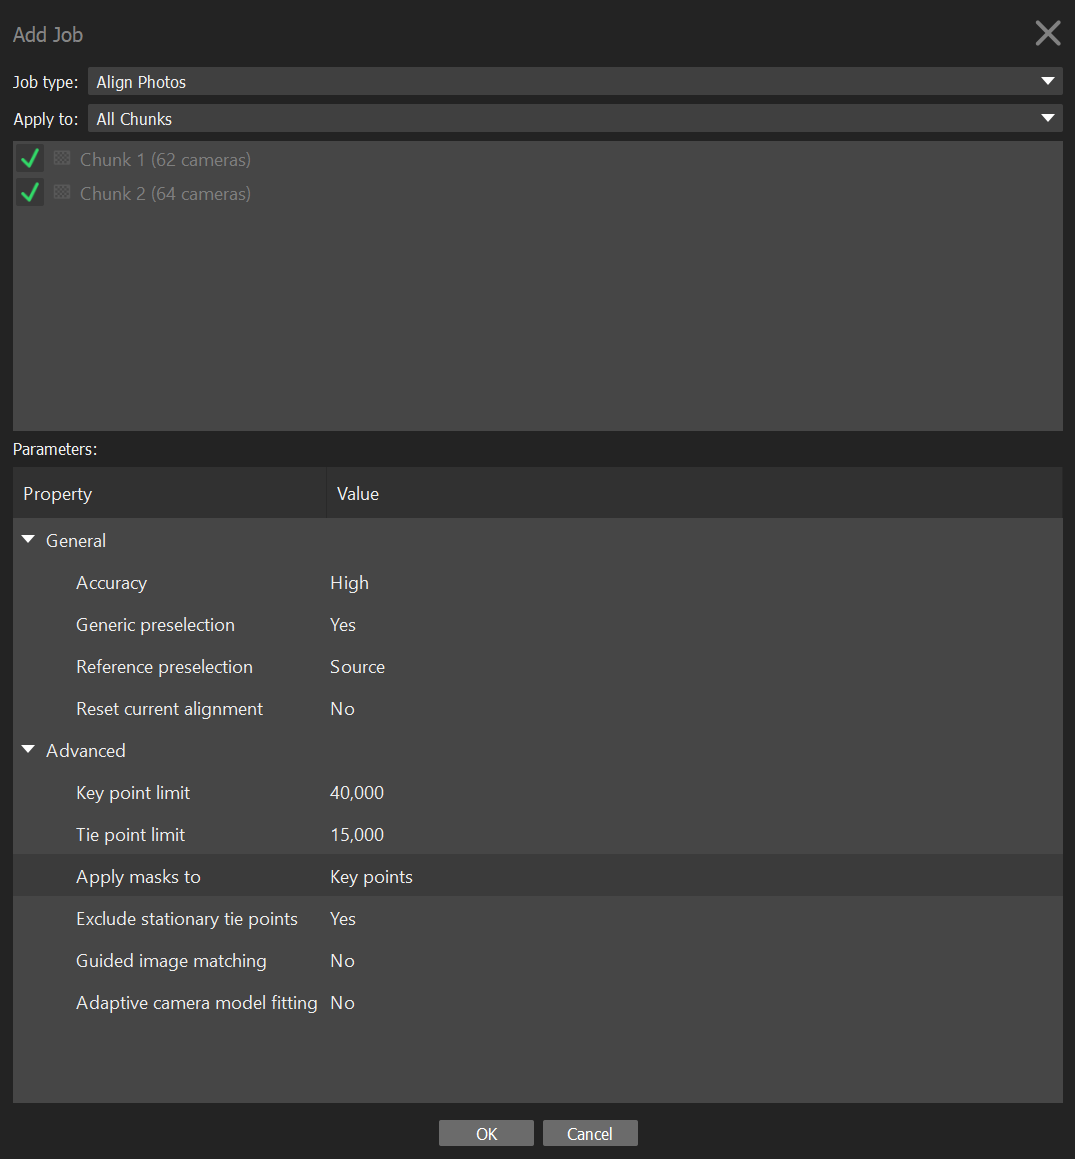
\includegraphics[width=0.5\textwidth]{Figures/metashape_batch_align.png}
    \caption{Align photos in multiple chunks}
    \label{batch_alignment}
\end{figure}

    \item \textbf{Optional: align using markers} If the different camera cannot align properly, it is possible to place homologous markers on the flower, defined as remarkable points on the flower (distinguishable pattern such as color dots on the corolla, for example), or by little pen marks at the surface of the flower when homologous markers lacks. These points need to be clearly identifiable on all camera groups. You will need at least 5 markers per flower, ideally positioned in different regions of the flower (e.g., near the peduncle, sepals tips, petals). Do not use points from the background to align chunks as it is independent from the flower (the flower changes position relative to the background).
    \begin{enumerate}
        \item Right click on the picture
        \item Then click on \textit{Place Marker} > \textit{New Marker}.
        \item In the left panel, rename them accordingly. Make sure to use the same nomenclature on each chunk to be able to merge them according to their names.
    \end{enumerate}
    \item To help the software recognize the markers, spread the manual markers on photos throughout the chunk (It is normally sufficient to place it on 2-3 photos and the software normally places them properly on the others, but make sure the markers are all properly placed).
    \item Repeat the step for each marker and each chunk. 
    \item Select one chunk. Go to \textit{Workflow > Align Chunks}, select the chunks you want to align, set the method as \textit{Markers based} and then click \textit{OK}. Repeat for all chunks to align.


    \item \textbf{Optional} If the camera alignment is not satisfactory, it is possible to clean the tie point obtained and try to realign the cameras. For instance, on the tie point generated by the alignment, you can delete outlier and imprecise points (Figure \ref{removing_points}): 
    \begin{enumerate}
        \item In the top menu, click on \textit{Model} and then \textit{Gradual Selection}. Select \textit{Reconstruction uncertainty} on \textit{Criterion} and play with the \textit{Level} value to remove the uncertain points. The higher the value, the worst is the point placed. Values between 30 and 10 generally give good results. Then \textit{OK}. Press \textit{Delete} on your keyboard to delete the selected points in red. You don't need much more than 10,000 points for good photo alignments.
        \item After removing uncertain points, go to the \textit{Reference} panel and click on \textit{Optimize Camera} to optimize camera position. Select all of the cameras. 
        \item In \textit{Model > Gradual Selection}, ensure that \textit{Reprojection error} parameter is below 1. If it is not, check if the alignment runs well (camera needs to form a full circle above the object). If the alignment fails, try to re-align photos by following step 3 (don't forget to check the box "reset current alignment"). If the alignment didn't fail, go to \textit{Model > Gradual Selection > Reproduction error}, and set the level to 1 and click OK. Then press \textit{Delete}. 
        \item Manually remove remaining outliers using the selection tool.
    \end{enumerate} 
    \item Repeat these steps for each chunk.
\end{enumerate}

\begin{figure}[H]
\begin{subfigure}[t]{.45\textwidth}
  \centering
  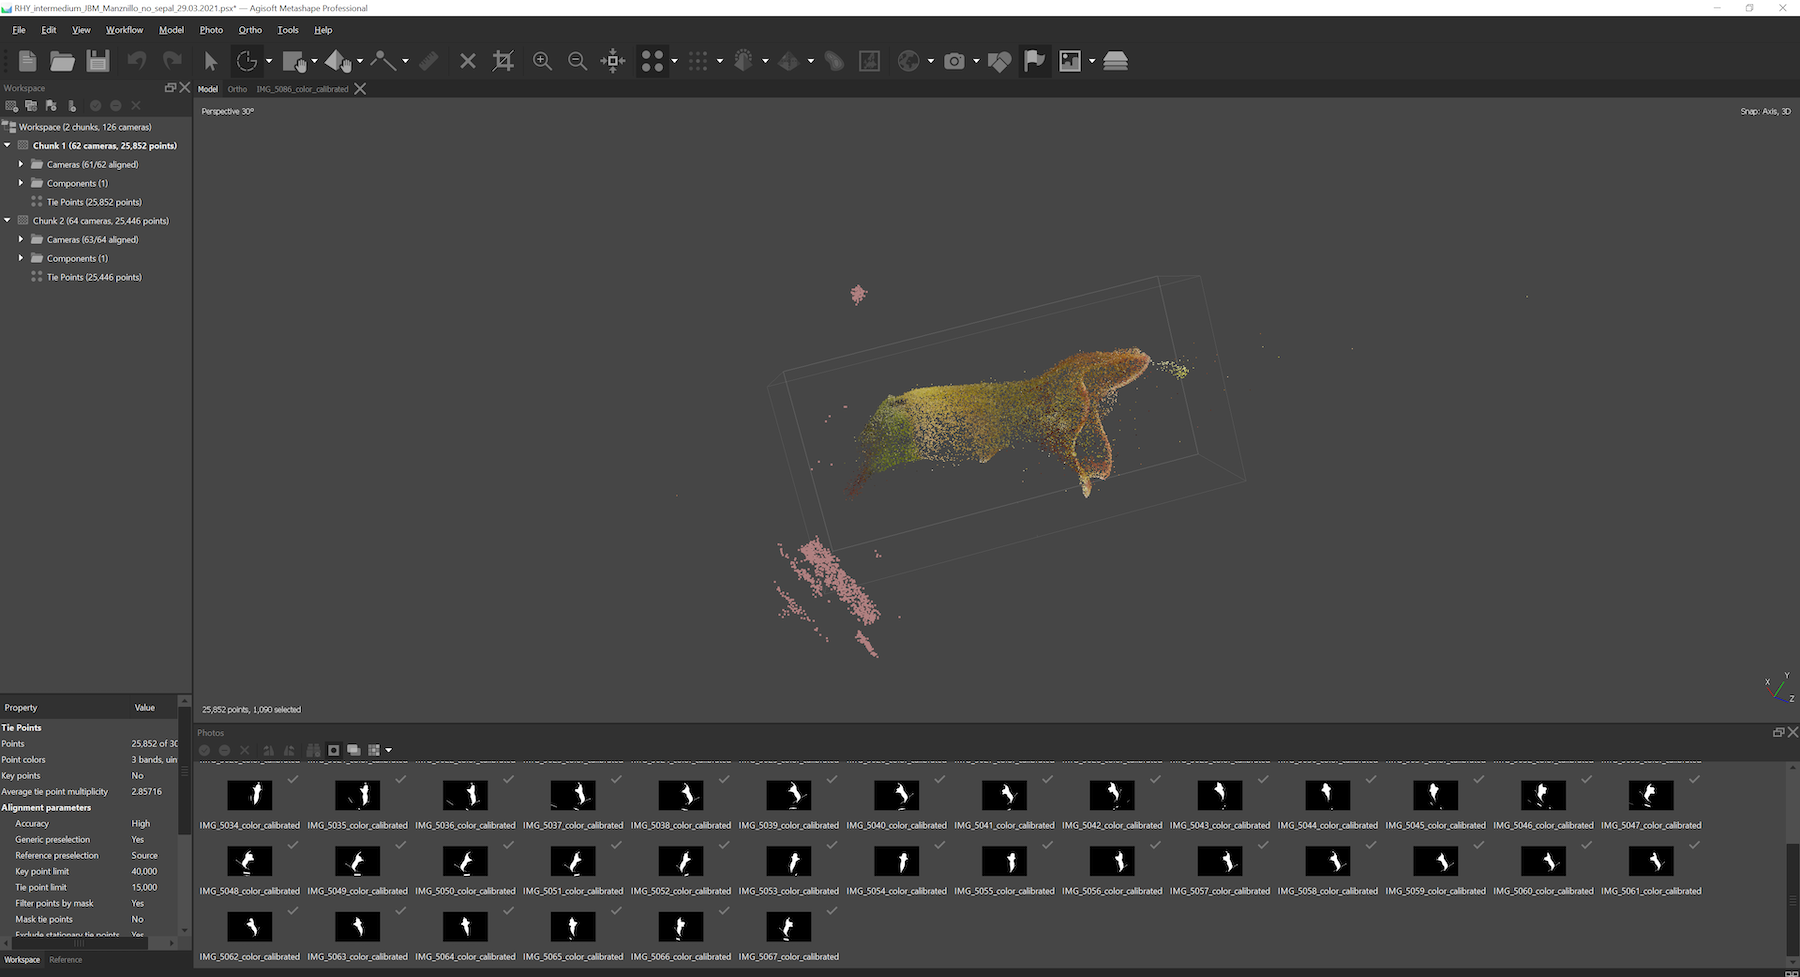
\includegraphics[width=1\textwidth]{Figures/metashape_delete_selectedpoints.png}
  \caption{Use the selection tool to remove background points}
  \label{model_orientation1}
\end{subfigure}%
\hfill
\begin{subfigure}[t]{.45\textwidth}
  \centering
  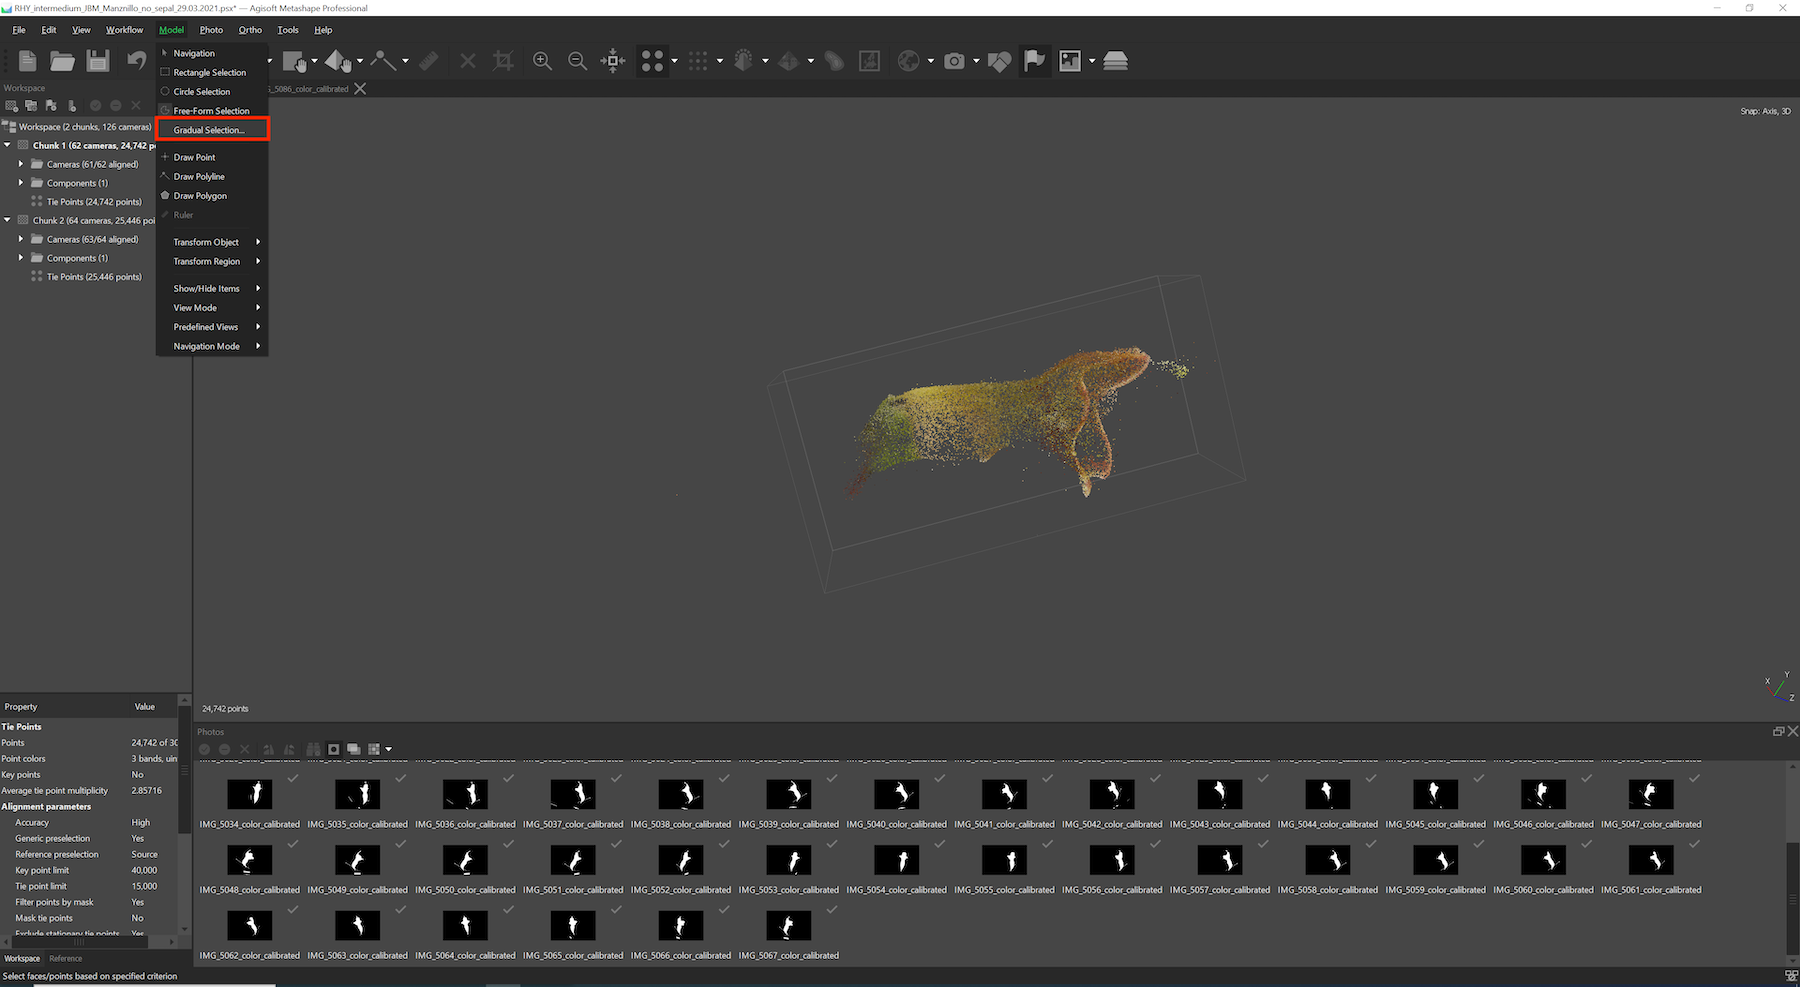
\includegraphics[width=1\textwidth]{Figures/metashape_gradual_selection.png}
  \caption{Use the gradual selection tool to remove additional mis-calculated points}
  \label{model_orientation2}
\end{subfigure}
\caption{Removing imprecise points}
\label{removing_points}
\end{figure}


\noindent \textbf{Note: If the alignment fails using only one chunk and two or more camera groups, then it will be necessary to divide your job in several chunks. Each chunk should then contain photos from one flower position. Once the chunks are ready, you can proceed with the alignment following the previous steps.}


\subsection{Align chunks together}

\noindent \textbf{Note: This step is only necessary if your project is divided in several chunks.}


At this step, it is important to align the different chunks with each other before they can be combined in a complete model. There are two ways to do this. The approach using tie points is quick but does not work all the time. If it fails, you will have to use the approach using markers.


\noindent To align using tie points :
\begin{enumerate}
    \item Select the chunks to align together.
    \item Go to \textit{Workflow} > \textit{Align Chunks}, select the chunks you want to align together, set the method as \textit{Point based} (Figure \ref{Align_chunk}).
    \item Restrict the key points with masks.
    \item Click on \textit{OK}.
\end{enumerate}


\noindent To align using markers :
\begin{enumerate}
    \item Place homologous markers on the flower, defined as remarkable points on the flower (distinguishable pattern such as color dots on the corolla, for example), or by little pen marks at the surface of the flower when homologous markers lacks. These points need to be clearly identifiable on all chunks. You will need at least 5 markers per flower, ideally positioned in different regions of the flower (e.g., near the peduncle, sepals tips, petals). Do not use points from the background to align chunks as it is independent from the flower (the flower changes position relative to the background).
    \begin{enumerate}
        \item Right click on the picture
        \item Then click on \textit{Place Marker} > \textit{New Marker}.
        \item In the left panel, rename them accordingly. Make sure to use the same nomenclature on each chunk to be able to merge them according to their names.
    \end{enumerate}
    \item To help the software recognize the markers, spread the manual markers on photos throughout the chunk (It is normally sufficient to place it on 2-3 photos and the software normally places them properly on the others, but make sure the markers are all properly placed).
    \item Repeat the step for each marker and each chunk. 
    \item Select one chunk. Go to \textit{Workflow > Align Chunks}, select the chunks you want to align, set the method as \textit{Markers based} and then click \textit{OK}. Repeat for all chunks to align.
\end{enumerate}

When the chunks are aligned, a [T] is put at the end of your chunk name to notify that it is transformed. You can check the alignment using the icon to show aligned chunks (icon of layers on top of each others, Figure \ref{show_aligned_chunk}). 
The different chunks should be well aligned over the whole flower.
If the alignment of your chunks is unsatisfactory, try to place more markers on recognizable features and spread across the whole flower. Additionally, you can manually align chunks using the tools to move the models in the space, but this is highly not recommended.



\begin{figure}[H]
\begin{subfigure}{.4\textwidth}
  \centering
  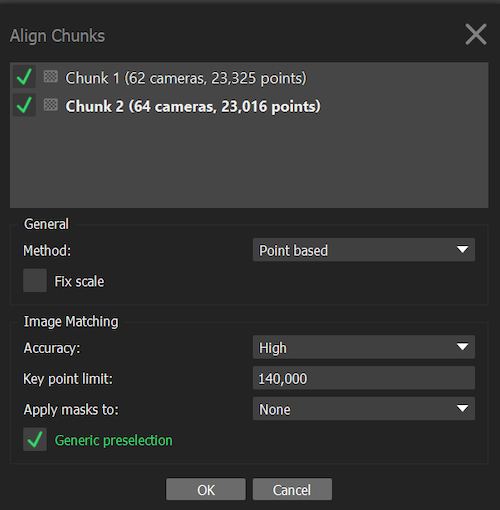
\includegraphics[width=1\textwidth]{Figures/metashape_align_chunks.png} %%%%% MISSING THE APPLY MASKS PARAMETER
  \caption{Align chunks}
  \label{Align_chunk}
\end{subfigure}
\begin{subfigure}{.7\textwidth}
  \centering
  \includegraphics[width=0.9\textwidth]{Figures/metashape_show_aligned_chunks.png}
  \caption{Show aligned chunks to verify their positions}
  \label{show_aligned_chunk}
\end{subfigure}
\caption{Chunk alignment}
\label{Chunk_alignment}
\end{figure}


\subsection{Merge chunks}

\noindent \textbf{Note: This step is only necessary if your project is divided in several chunks.}

The next step is to merge chunks together when they are well aligned. Click on \textit{Workflow > Merge chunks}, and merge using either the tie point method or the markers method depending on the option selected above.

\subsection{Build 3D mesh}
\begin{enumerate}
    \item Select the chunk or the merged chunks for which you want to build a 3D mesh (model).
    \item Go to \textit{Workflow > Build Mesh}.
    \item In the dialog box, make sure that \textit{Source Data} is on \textit{Depth maps}, \textit{Quality} and \textit{Face Count} on \textit{High} (Figure \ref{fig:3d_mesh}). Note that although it is also possible to generate a mesh from a dense point cloud (which has to be built separately), the depth maps provide better results for objects with a high number of minor details.
    \item Then go to \textit{Advanced}, check \textit{Calculate vertex colors}. Click OK.
    \item Once the mesh is produced, you should remove the pin and extra floating background parts using the selection tool. This will highlight the selection in red.
    \item Verify your selection and press delete to remove them.
%try to remove unnecessary cameras : see p9 of the Metashape user guide.
\end{enumerate}

\begin{figure}[H]
    \centering
    \includegraphics[width=0.5\textwidth]{Figures/metashape_build_mesh.png}
    \caption{Build 3D mesh}
    \label{fig:3d_mesh}
\end{figure}

\begin{tcolorbox}[width=\linewidth, colback=mygray,title=Note on 3D mesh construction,colframe=lightgray]
Our protocol merges the chunks to build a tie point model of all chunks before constructing a model for the merge chunk. We found that this is the best approach, although it is also possible to build models for each chunk separately and then merge these models to obtain a full model.
\end{tcolorbox}



\subsection{3D mesh touch ups}
\begin{enumerate}
    \item You can smooth the mesh by clicking on \textit{Tools}, \textit{Mesh}, \textit{Smooth Mesh}. You can also duplicate a 3D model to save one intact, and right click on it, and un-check \textit{Use as default} to keep it as an archived model. If you smooth a mesh, you can't undo it.
    \item You can fill holes in your mesh by clicking on \textit{Tools > Mesh > Close Holes}. Note that if your holes are too big, the closing function can create unwanted structures. Similarly as the smoothing, you can't undo closing holes in the mesh. \textbf{HOWEVER}, this will remove the vertex colors in version 1.7.2, which we will need to place landmarks when doing the morphometrics.
\end{enumerate}


\subsection{Build texture}

To build the texture : \textit{Workflow > Build Texture}, use the preset values and click OK.



\subsection{Scaling}
\noindent To scale the model, go to the pictures of your merged chunk and follow these steps :
    \begin{enumerate}
        \item On a picture displaying the scale bar, add new markers at each end of the scale bar and on a couple of additional photos.
        \item In the left panel, select both markers and click on the icon \textit{Add scale} (Figure \ref{metashape_scale}). % Create Scale Bar
        \item Go to the \textit{Reference} panel, select the scale and add 0.01 as reference.
        \item Click on the \textit{Update transform} button (rotating arrows). This is an important step, because otherwise the scale will not be incorporated to your model.
        \item To verify if the scale is taken into account, you can use the measuring tape tool.
    \end{enumerate}

%FIGURES scale, measuring
\begin{figure}[H]
  \centering
  \includegraphics[width=0.9\textwidth]{Figures/metashape_add_scale_2.png}
  \caption{Add a scale using landmarks}
  \label{metashape_scale}
\end{figure}


\subsection{Model orientation}
    \begin{enumerate}
        \item In Metashape, be sure that \textit{Show info} in \textit{Model > Show/Hide Items} is checked. You should see at the bottom right of the model panel the 3D axes. 
        \item Show grid
        \item Make sure that the scale is the right one, changing it will affect the coordinates of the 3D model. You can verify the scale using the measuring tool. 
        \item Use the navigation tool to orient these 3D axes. 
        \item Once you orient the 3D axes in the wanted direction, you can then use the tool \textit{Rotate Object} to put the object in the wanted direction, and at the center of the grid, facing the right side of the grid.
        \item Orient the binding box as well with the cross on the ventral side, and the two dash facing the opening of the flower. Note that depending on the software you use to open the model, the first view orientation may change when you open the final object file.
    \end{enumerate}


%FIGURE

\begin{figure}[H]
\centering
\begin{subfigure}{0.9\textwidth}
  \centering
  \includegraphics[width=1\textwidth]{Figures/metashape_orientation.png}
  \caption{}
  \label{}
\end{subfigure}

\begin{subfigure}{0.9\textwidth}
  \centering
  \includegraphics[width=1\textwidth]{Figures/metashape_orientation_2.png}
  \caption{}
  \label{}
\end{subfigure}
\caption{Metashape 3D axes and flower orientation}
\label{flower_orientation}
\end{figure}






\subsection{Export model and texture}
 


\begin{enumerate}
    \item You can export your 3D model by clicking on \textit{File} > \textit{Export} > \textit{Export Model}.
    \item Name your model
    \item Choose .ply as the extension.
    \item In the dialog box, tick the \textit{Vertex colors}. This option will allow you to get color on the actual 3D model.
    \item Select \textit{Export texture} as PNG.
    \item Make sure to export the texture with transparency, by ticking the \textit{Write alpha channel} option. The texture is a separate file, with detail color information that is wrapped on the model.
    \item Click on \textit{OK}.
\end{enumerate}

% \subsection{Export mesh from .obj file to .ply file}
% Convert the .obj file obtained from Metashape to a .ply file readable in R.\\
% \textbf{Using Meshlab :}
% \begin{enumerate}
%     \item Download Meshlab here : %insert href link
%     \item Open MeshLab, click on "File" and "Import Mesh". A dialog box appears and you have to chose your .obj file.
%     \item Go to "File", "Export Mesh As". A dialog box appears and you need to name your file and chose the format .ply for your file.
%     \item After choosing the name and the file format, another dialog box appears. Make sure that all the boxes in "Vert", "Face" and "Wedge" are unchecked. On "Additional parameters" make sure that the two boxes are unchecked too. Only "All" must be checked. Click "OK". Your mesh is now compatible with R.
%     \end{enumerate}
% \textbf{Using Stratovan Checkoint :
% }








%THE NEXT SECTION IS REMOVED FROM THE PROTOCOL FOR NOW
%IT IS A BIT SPECIFIC TO GESNERIACEAE, NOT FOR GENERAL MORPHOMETRICS
%-------------




%commented out section
\begin{comment}
%-------------

\newpage
\section{3D Geometric morphometrics}

\subsection{Build the flower template in Meshlab}
Build a template is essential to easily apply surface semi-landmarks in Stratovan Checkpoint (see the next step).
\begin{enumerate} 
    \item In Meshlab, go to \textit{Filters}, select \textit{Create New Mesh Layer} and chose \textit{Cone}. Specify the value of radius 1 and 2 (this is the value of the top and bottom radius of the cone; if you want a cylinder just put the same value), the value of height and the number of sides.
     % Simon did the cone we use and I think the values were radius 1 = 1, radius 2 = 1.3, height = 2, sides = 36, but we can discuss and modify if needed.
    \item We need the template to be open at both top and bottom sides because we don't want to apply surface semi-landmarks in the corolla or on the flower stalk. In Meshlab, select the tool \textit{Select Faces in a Rectangular Region} and select the top and bottom cover of the cone then press delete. 
    \item You can now export the mesh going to \textit{File > Export Mesh As}, name your file and chose the non binary .ply extension, then \textit{Save}.
\end{enumerate}





\subsection{Place landmarks and semi-landmarks on the flower template in Stratovan Checkpoint}
Landmarks and semi-landmarks have to be placed in the exact same order as described in the table hereafter.
%screen captures
\begin{enumerate}
    \item  Open the template : in the "Specimen" tab, browse the file path destination and select the template on the left panel. Click on "Open specimen". Check on the Save icon to create a CKPT file (checkpoint) that will be used to reopen the project.
    \item Go to the tab surface and place the landmarks and semi-landmarks following these instructions
    \begin{enumerate}
        \item Select the landmark tool and place the petals landmarks : Depending on if you want to put surface landmarks on petals, you have to place the landmarks just below the top end (Fig. \ref{template_stratovan_a}) to let space for surface semi-landmarks. Place the semi-landmarks equidistant from each other. You need to remember the order of landmarks because you will have to place the landmarks on the flower in the same order later (see the next part). 
        \item  Rename your landmarks accordingly : in the surface tab, double click on a point and select 'rename primitive', or in the tab 'Landmarks', click on the skull icon to show the surface, and select your point, then you can rename it in the right panel.
        \item Now, place the curve semi-landmarks according to table 3. For example, the dorsal curve have 20 points and the first one is common (merged) with the landmarks 1. The ventral curve have 20 points and the first one is common (merged) with the landmarks 8. Curves from margin have 21 points and the extremity points are merged with landmarks of petals or sepals. Rename the curve semi-landmarks as mentioned in table 3 in the "Landmarks" tab. 
        \item On the template, we need to place the surface semi-landmarks for the tube. Select the grid tool, and place the grid on a half cylinder. Go to the "Landmarks" tab, chose "Patch" in the drop down menu, and select the patch you just create. Select X = 13 and Y = 21 or X = 21 and Y = 13 depending on how you place the grid. 21 is the width, 13 is the height (Fig. \ref{template_stratovan_b}). You can now fit the grid on the half cylinder ensuring that the space between the point are equal. None of the points of the grid are merged. Once the grid is placed as desired, repeat this step by adding another grid on the other half of the cylinder. Rename the patches as mentioned in table 3 in the "Landmarks" tab.
        \item On the template, we also need to place the surface semi-landmarks for the petals. Select the grid tool, and place the grid between two petal landmarks. Go to the "Landmarks" tab, chose "Patch" in the drop down menu, and select the patch you just create. Select X = 13 and Y = 5 or X = 5 and Y = 13 depending on how you place the grid. 13 must be the width and 5 the height (Fig. \ref{template_stratovan_b}). You can now fit the grid between the two petal landmarks (Fig. \ref{template_stratovan_a}). None of the points of the grid are merged, but this time you have to place the guided semi-landmarks (with an arrow) of both left and right side of the patch at the same position than the landmarks from left and right side respectively. This allow to give to the patch a shape close to the petals. Once the grid is placed as desired, repeat this step for each petal. Rename the patches as mentioned in table 3 in the "Landmarks" tab.
        \item Verify order and line number of each landmark in the listing by viewing the landmarks list in export>landmarks>csv
        \item When you are done, export surface in PLY format, and the data in CSV and NTSF format.
       
    \end{enumerate}
\end{enumerate}

 \begin{figure}[h]
\centering
\begin{subfigure}[t]{.45\linewidth} % >>> [t] -> helps aligning subfigures according to the image not the text
 \centering
  \includegraphics[width=1\linewidth]{Figures/checkpoint_landmarks_low.png}
  \caption{Landmarks placed below the top end of the template to let space for petal surface semi-landmarks. We can also see the patch placed on the top end of the template to represent the petal}
  \label{template_stratovan_a}
 \end{subfigure}\hspace{10pt}%
\vspace{10pt}
\begin{subfigure}[t]{.45\linewidth}
  \centering
  \includegraphics[width=1\linewidth]{Figures/chekcpoint_patch_tube.png}
  \caption{Template and patch placed on a half cylinder representing the corolla tube}
  \label{template_stratovan_b}
\end{subfigure}\hspace{10pt}%
 \caption{Template and position of landmarks}
  \label{template_stratovan}
\end{figure}






%old figure
%\begin{figure}[h]
%\centering
%\includegraphics[width=0.4\textwidth]{Figures/template_stratovancheckpoint.png}
%\caption{}
%\label{template}
%\end{figure}

\subsection{Place landmarks and semi-landmarks on flowers}


Landmarks and semi-landmarks have to be placed in the exact same order as described in the table hereafter.

%It seems to be better to store the ply files (exported from Stratovan) files and the CKPT files together to be able to open one or the other project from the same checkpoint session.

\begin{enumerate}
    \item Open model : in the tab Specimen, Browse the file path destination, select your file on the left panel, and click on the Open Specimen button on the right panel. Check on the Save icon to create a CKPT file (checkpoint) that will be used to reopen the project.
    \item In the tab Surface, select the landmark tool, and place the landmarks at the petal intersections, and sepal intersections.
    \item Rename your landmarks accordingly : in the surface tab, double click on a point and select 'rename primitive', or in the tab 'Landmarks', click on the skull icon to show the surface, and select your point, then you can rename it in the right panel.
    \item Curves are guided by the landmarks placements, and their direction is important. Place the first curves on the dorsal then ventral sections. The dorsal one starts at the first landmark (Petal 1) and the second one starts at the sepal intersection (Sepal 3).
    \item Verify order and line number of each landmark in the listing by vewing the landmarks list in export>landmarks>csv
    %\item for curves, you can place 5 semi landmarks manually and define the curve to have 10 landmarks (5 automatically placed between manual semi landmarks) in landmarks> (screen capture) (verify, but 10 manual semi landmarks to get in total 20 semi-landmarks for petal margins for example) (for the dorsal and ventral curves, you can place only 2 landmarks and fill in with the defined number of landmarks).
    %insert descriptive table of landmark names and number and a figure for their position : side by side a graphical illustration + model
    \item When you are done, export surface in PLY format with binary encoding unchecked to use the ASCII format, and set the scale in cm
    \item Export the data in NTSF format, using the scale in cm.
    \item The .nts files written by Stratovan Checkpoint have incorrect headers. Replace manually the header of the .nts files to work in R from the default format 1 n p-x-k 1 9999 Dim=3 to the modified format 1 n p-x-k 0 Dim=3 to avoid NAs to be introduced as virtual missing data. \\ In our case : change the second header line from \textbf{1 729 1 9999 Dim=3} to \textbf{1 243 3 0 dim=3} 
\end{enumerate}







\begin{figure}[H]
\centering
\begin{subfigure}[t]{1\textwidth}
  \centering
  \includegraphics[width=.6\textwidth]{Figures/stratovan_curves_petals.png}
  \caption{Curves for overlapping petals}
  \label{}
\end{subfigure}

\begin{subfigure}[t]{1\textwidth}
  \centering
  \includegraphics[width=.6\textwidth]{Figures/stratovan_landmarks_curves_basepetals_2.png}
  \caption{Dorsal, petals, and sepal curves}
  \label{}
\end{subfigure}

\begin{subfigure}[t]{1\textwidth}
  \centering
  \includegraphics[width=.6\textwidth]{Figures/stratovan.png}
  \caption{The curves for the basis of petals are not straight. Follow the crease in the corolla.}
  \label{}
\end{subfigure}

\caption{Curve positions in Stratovan}
\label{}
\end{figure}













\noindent Protocol details for potential problems  encountered :
\begin{enumerate}
    \item %for fringed petal margin, how to place points
    \item%for very curved back petals, how to place curves
    \item%for missing landmarks, or confusing landmarks
    \item%when sepal intersections are confusing, refer to the textured model
    \item%placement of close points will fuse, to avoid
    \item %for overlapping petals (especially the top ones).
\end{enumerate}












%screen captures


%Table
\begin{table}[H]
\centering
\caption{Landmark IDs (names), point ID (number) and number of point per curves, including sliders (sliding semi-landmarks) for each landmark and curve. Landmarks (red) and semi-landmarks for curves (yellow) and surfaces (blue).}
\begin{tabular}{llll}
\rowcolor[HTML]{F3F3F3} 
\textbf{Landmark ID} & \textbf{point ID} & \textbf{npoints} & \textbf{nsliders} \\
{\color[HTML]{EA4335} \textbf{Petal 1}} & 1 & 1 &  \\
{\color[HTML]{EA4335} \textbf{Petal 2}} & 2 & 1 &  \\
{\color[HTML]{EA4335} \textbf{Petal 3}} & 3 & 1 &  \\
{\color[HTML]{EA4335} \textbf{Petal 4}} & 4 & 1 &  \\
{\color[HTML]{EA4335} \textbf{Petal 5}} & 5 & 1 &  \\
\hline
{\color[HTML]{EA4335} \textbf{Sepal 1}} & 6 & 1 &  \\
{\color[HTML]{EA4335} \textbf{Sepal 2}} & 7 & 1 &  \\
{\color[HTML]{EA4335} \textbf{Sepal 3}} & 8 & 1 &  \\
{\color[HTML]{EA4335} \textbf{Sepal 4}} & 9 & 1 &  \\
{\color[HTML]{EA4335} \textbf{Sepal 5}} & 10 & 1 &  \\
\hline
%Even if stigmat landmarks are placed after the curves, CHeckpoint groups landmarks before semi-landmarks of curves.
% {\color[HTML]{EA4335} \textit{\textbf{Stigmat 1}}} & 11 & 1 &  \\
% {\color[HTML]{EA4335} \textit{\textbf{Stigmat 2}}} & 12 & 1 &  \\
% {\color[HTML]{EA4335} \textit{\textbf{Stigmat 3}}} & 13 & 1 &  \\
% {\color[HTML]{EA4335} \textit{\textbf{Stigmat 4}}} & 14 & 1 &  \\
% \hline
%%%%%% REDEFINE SEMI LANDMARK NUMBER BECAUSE THE ADDITIONAL STIGMAT LANDMARKS SLIDE EVERYTHING 4 RANKS AHEAD. %%%%%%%%%%
    %%For dorsal and ventral curves : place 2 points and define 19 landmarks in the Landmarks tab  
{\color[HTML]{FBBC04} \textbf{Curve dorsal}} & 1,11:29 & 20 & 19 \\ 
{\color[HTML]{FBBC04} \textbf{Curve ventral}} & 8, 30:48 & 20 & 19 \\
\hline
    %For petal margins : place 7 points manually and define a total of 19 landmarks in the Landmarks tab
{\color[HTML]{FBBC04} \textbf{Curve margin Petal1-Petal2}} & 1,49:67,2 & 21 & 19 \\ 
{\color[HTML]{FBBC04} \textbf{Curve margin Petal2-Petal3}} & 2,68:86,3 & 21 & 19 \\
{\color[HTML]{FBBC04} \textbf{Curve margin Petal3-Petal4}} & 3,87:105,4 & 21 & 19 \\
{\color[HTML]{FBBC04} \textbf{Curve margin Petal4-Petal5}} & 4,106:124,5 & 21 & 19 \\
{\color[HTML]{FBBC04} \textbf{Curve margin Petal5-Petal1}} & 5,125:143, 1 & 21 & 19 \\
\hline
    %For sepal curves : place 2 points and define 5 landmarks
{\color[HTML]{FBBC04} \textbf{Curve Sepal1-Sepal2}} & 6,144:148,7 & 7 & 5 \\ 
{\color[HTML]{FBBC04} \textbf{Curve Sepal2-Sepal3}} & 7,149:153,8 & 7 & 5 \\
{\color[HTML]{FBBC04} \textbf{Curve Sepal3-Sepal4}} & 8,154:158,9 & 7 & 5 \\
{\color[HTML]{FBBC04} \textbf{Curve Sepal4-Sepal5}} & 9,159:163,10 & 7 & 5 \\
{\color[HTML]{FBBC04} \textbf{Curve Sepal5-Sepal1}} & 10,164:168,6 & 7 & 5 \\
\hline
    %For the base of petals : place 3 landmarks and define 15
{\color[HTML]{FBBC04} \textbf{Curve base Petal1-Petal2}} & 1,169:183,2 & 17 & 15 \\
{\color[HTML]{FBBC04} \textbf{Curve base Petal2-Petal3}} & 2,184:198,3 & 17 & 15 \\
{\color[HTML]{FBBC04} \textbf{Curve base Petal3-Petal4}} & 3,199:213,4 & 17 & 15 \\
{\color[HTML]{FBBC04} \textbf{Curve base Petal4-Petal5}} & 4,214:228,5 & 17 & 15 \\
{\color[HTML]{FBBC04} \textbf{Curve base Petal5-Petal1}} & 5,229:243,1 & 17 & 15 \\
\hline
{\color[HTML]{4285F4} \textbf{Surface tube}} & 244:789 &  &  \\
{\color[HTML]{4285F4} \textbf{Surface petal 1}} & 790:844 &  &  \\
{\color[HTML]{4285F4} \textbf{Surface petal 2}} & 845:899 &  &  \\
{\color[HTML]{4285F4} \textbf{Surface petal 3}} & 900:954 &  &  \\
{\color[HTML]{4285F4} \textbf{Surface petal 4}} & 955:1009 &  &  \\
{\color[HTML]{4285F4} \textbf{Surface petal 5}} & 1010:1064 &  &  \\
\hline


%\hline
%{\color[HTML]{EA4335} \textit{\textbf{Etamin 1}}} & 1069 &  &  \\
%{\color[HTML]{EA4335} \textit{\textbf{Etamin 2}}} & 1070 &  &  \\
%{\color[HTML]{EA4335} \textit{\textbf{Etamin 3}}} & 1071 &  &  \\
%{\color[HTML]{EA4335} \textit{\textbf{Etamin 4}}} & 1072 &  &  \\

\end{tabular}
\end{table}




%%%%%%%the following section is not needed in this protocol but we can keep the figure to have an overview of the results we get in the end.
\subsection{Apply template to flowers for surface points in R}

\begin{figure}[H]
\centering
\begin{subfigure}[t]{.5\textwidth}
  \centering
  \includegraphics[width=.5\textwidth]{Figures/template_geometric_morphometrics.png}
  \caption{}
  \label{}
\end{subfigure}% -> this % allows the graphs to be side by side as opposed to one on top of the other
\begin{subfigure}[t]{.5\textwidth}
  \centering
  \includegraphics[width=.5\textwidth]{Figures/flower_geometric_morphometrics.png}
  \caption{}
  \label{}
\end{subfigure}
\caption{}
\label{}
\end{figure}



%-------------
\end{comment}
%-------------




%BIBLIOGRAPHY
\newpage
\bibliography{references.bib}
\end{document}






%%%%%%%%%%%%%%%%%%%%%%%%%%%%%%%%%%%%%%%%%%%%%%%%%
%%  CHECKLIST OF THINGS TO ADD IN THE PROTOCOL %%
%%%%%%%%%%%%%%%%%%%%%%%%%%%%%%%%%%%%%%%%%%%%%%%%%

%how to orient the models / how to set the origin of the coordinates axes 

%how to export videos of models + how to change the background of the video to export

%clarify how to export models : .obj vs. .ply and ASCII vs. binary for the .ply ones. 

%there are several figures needed : search for the keyword %FIGURES

% Verify if tiny holes are an issue in the surface semi landmarks placement. Try to use Metashape or Blender to fill these holes.


%%%%%%%%%%%%%%%%%%%%%%%%%%%%%%%%%%%%%%%%%%%%%%%%%
%%  NOTES MEETING 14 DEC. 2021 %%
%%%%%%%%%%%%%%%%%%%%%%%%%%%%%%%%%%%%%%%%%%%%%%%%%

%use calibration groups instead of chunks, more eficient, compute all in one and avoid aligning chunks with each others.
%on oublie le dense cloud, et le nettoyage des points sur le tie point cloud
%ne pas nettoyer de façon agressive, mild ou moderate
%ajouter l'outil de selection automatique : lasso en maintenant ctrl
%si pas de masque partout, effet sur la texture (zones floues). pas necessaire d'en mettre partout autrement.
%reference preselection / source vs. estimated -> vérifier si c'est pour les coord. gps des cameras , ou la position de sphotos (l'ordre des photos).
%sclaing : important
%orientation -> trouver une façon plus simple, car pas facile autrement manuellement. trouver une facon de changer les coordonnées du repère.
%appareil photo qui fait du stack focusing automatiquement ? 
% camera qui fait un meilleur autofocus ?
%protocole compatible avec ce qui est fait dans l'article
